% Going off the Thesis guidelines available here: http://www.lboro.ac.uk/students/welcome/research/codes-of-practice/appendices/
% A4 paper size selected, default is 11pt font, to change to 12pt use [a4paper, 12pt] as option to documentclass
\documentclass[a4paper]{report}

% Some useful packages for including images, colored font, etc.
\usepackage[dvips]{graphicx}
\graphicspath{{Figures/}}

\makeatletter
\def\maxwidth{\ifdim\Gin@nat@width>\linewidth\linewidth\else\Gin@nat@width\fi}
\def\maxheight{\ifdim\Gin@nat@height>\textheight\textheight\else\Gin@nat@height\fi}
\makeatother
\setkeys{Gin}{width=\maxwidth,height=\maxheight,keepaspectratio}
\usepackage{amssymb,amsmath}
\usepackage{longtable}
\usepackage{booktabs}

\usepackage{listings}
\usepackage{xcolor}
 
\definecolor{codegreen}{rgb}{0,0.6,0}
\definecolor{codegray}{rgb}{0.5,0.5,0.5}
\definecolor{codepurple}{rgb}{0.58,0,0.82}
\definecolor{backcolour}{rgb}{0.95,0.95,0.92}
 
\lstdefinestyle{mystyle}{
    backgroundcolor=\color{backcolour},   
    commentstyle=\color{codegreen},
    keywordstyle=\color{magenta},
    numberstyle=\tiny\color{codegray},
    stringstyle=\color{codepurple},
    basicstyle=\ttfamily\footnotesize,
    breakatwhitespace=false,         
    breaklines=true,                 
    captionpos=b,                    
    keepspaces=true,                 
    numbers=left,                    
    numbersep=5pt,                  
    showspaces=false,                
    showstringspaces=false,
    showtabs=false,                  
    tabsize=2
}
 
\lstset{style=mystyle}

\usepackage[numbers]{natbib}

\usepackage{color}
\usepackage{url}
\usepackage{subcaption}
\usepackage{pdflscape}

% Global bibliography style
\bibliographystyle{unsrt}

% Set margins in all document to 3.5cm as per guidelines for binding
\usepackage[includeheadfoot,margin=3.5cm]{geometry}

% Used to including pdf files within pages
% use [draft] as option to output empty spaces rather than rendering all pages (useful when including lots of pdfs)
\usepackage{pdfpages}

% Used to produce headers and footers
\usepackage{fancyhdr}
\pagestyle{fancyplain}

% Used for removing title in bibliography sections
\usepackage{titlesec}

% Used to generate lists of abbreviations
\usepackage{nomencl}
\makenomenclature 
\renewcommand{\nomname}{List of Abbreviations}

% To have a separate bibliography per Chapter uncomment this line
% See Introduction/Introduction.tex for example how to include the bibliography
%\usepackage{chapterbib}

% Line spacing defined at 1 and a half. I know it says 1.3 but its 1 and a half.
\linespread{1.3}

% Setup headers and footers
\fancyhf{}
\lhead{\leftmark}
% Center on all pages
% \fancyhead[C]{---Draft---}
% Page number placed on right side on odd pages and left side on even pages
\fancyfoot[RO, LE] {\thepage}


\begin{document}

% Give \subsubsection numbers
\setcounter{secnumdepth}{4}

% Title, Author, Abstract, Acknowledgement, Table of Content, List of Figures, List of Tables and List of Abbreviations
% Front matter of the Thesis
% Title page
% Loughborough University Thesis Access Form
% Loughborough University Certificate of Originality
% Abstract
% Acknowledgements
\title{\bf Building BT Network}

\author{by\\
Zhihao DAI\\
Yunsong ZHANG\\
Huijing LEI\\
Changrong CHEN\\
Yan HUANG\\
\\
{\bf 19COP502 Building Secure Networks}\\
{\bf Lab Report}\\
\\
Loughborough University\\
\\
\copyright
\hspace{1 dd} BT NETWORK 2019\\
\\
Nov. 2019
}
\date{} % Used to remove date from title so it can be set at any date rather than the current date

\maketitle

% Set page numbers to roman numerals for front matter
\pagenumbering{roman}

% % PDF exports of Word Documents available (Exported August 2012)
% % Thesis Access Form
% 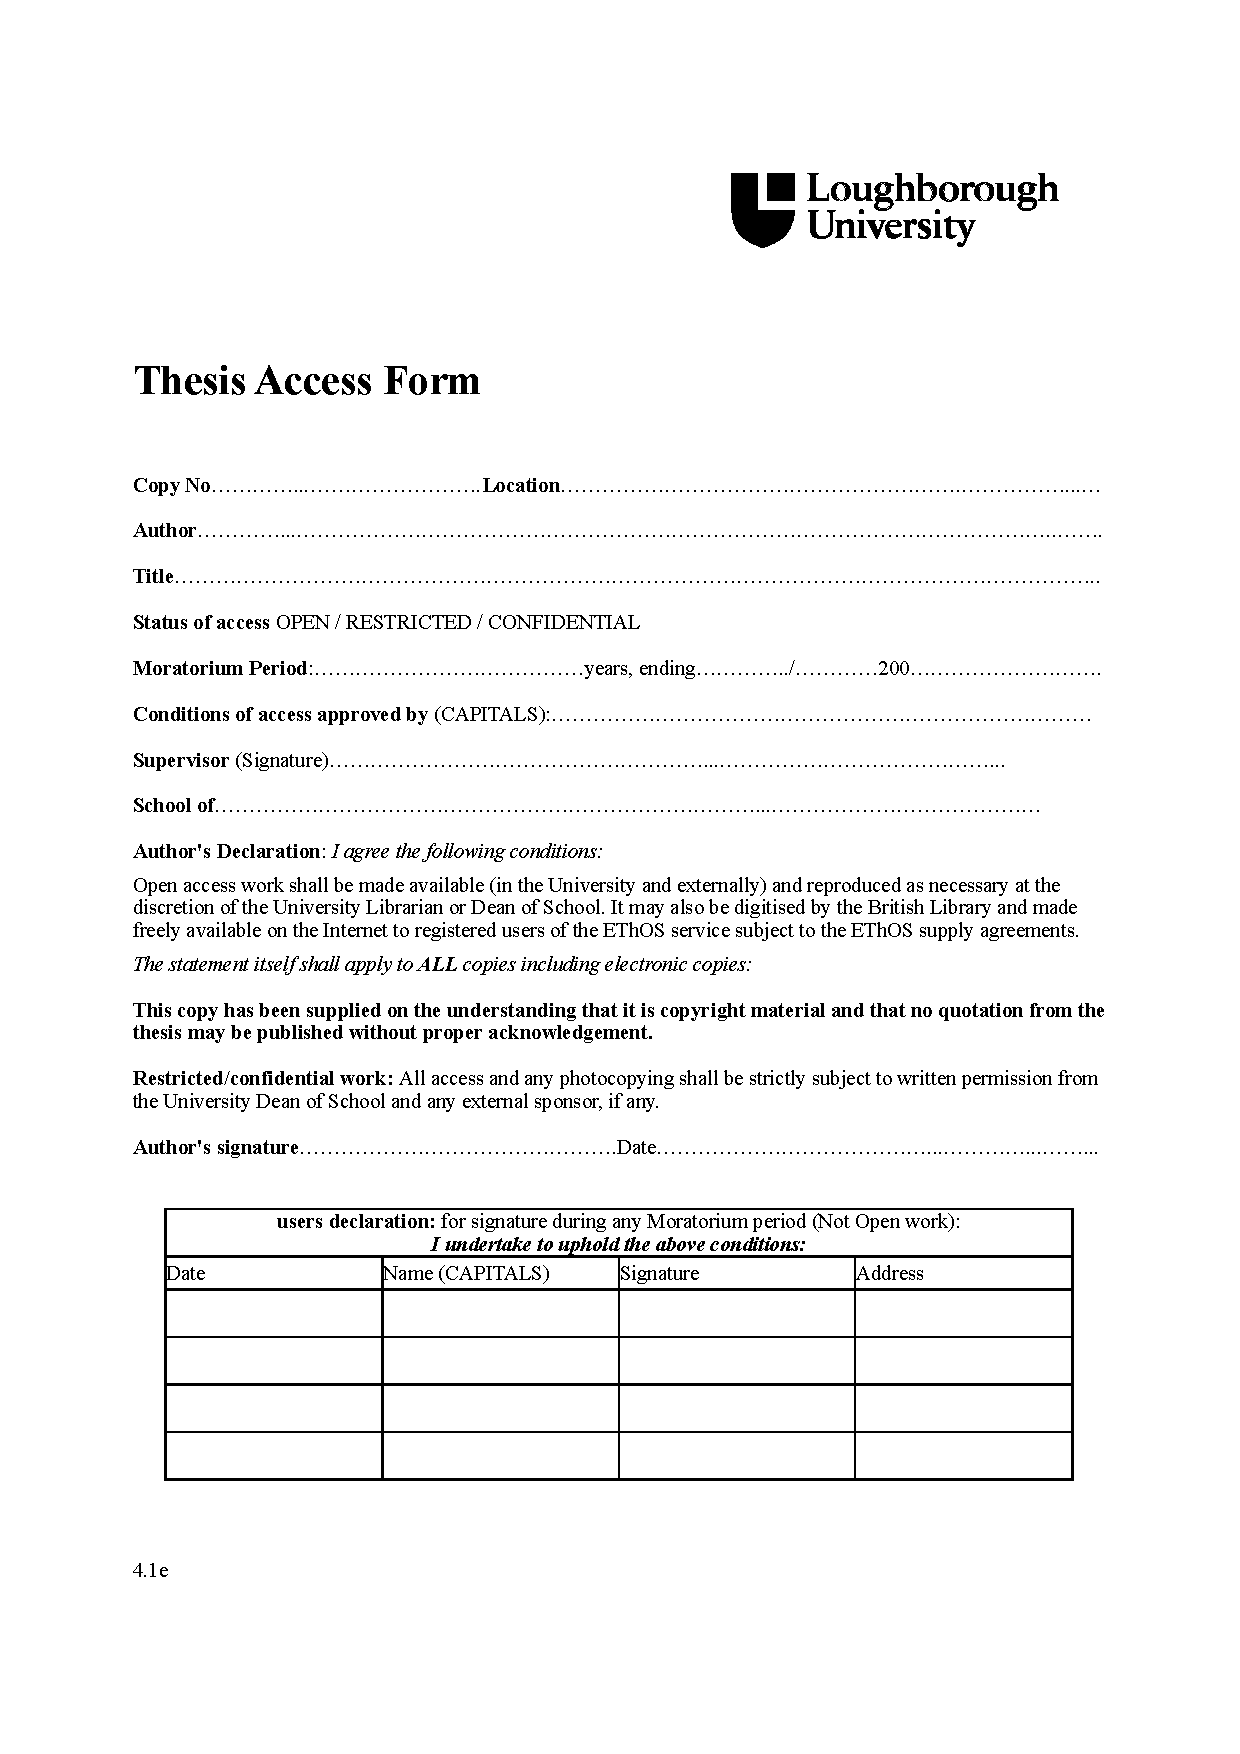
\includepdf[pages=1, pagecommand=, templatesize={5in}{10in}]{Front/LU/access.pdf}
% % Certificate of Originality
% 
\includepdf[pages=-, pagecommand=, templatesize={5in}{10in}]{Front/LU/origin.pdf}

% Abstract
\addcontentsline{toc}{chapter}{Abstract}
\chapter*{Abstract}
TODO


% % Acknowledgements
% \addcontentsline{toc}{chapter}{Acknowledgements}
% \chapter*{Acknowledgements}
% Acknowledgement section.

% Set the depth for your table of content
% Currently set at 2 (Chapter, Section, Subsection)
\setcounter{tocdepth}{2}
% Include a table of content
\tableofcontents

% Include a list of figures
\addcontentsline{toc}{chapter}{List of Figures}
\listoffigures

% Include a list of tables
\addcontentsline{toc}{chapter}{List of Tables}
\listoftables

% Include a list of abbreviations using nomenclature package
%\addcontentsline{toc}{chapter}{List of Abbreviations}
%\printnomenclature[3cm] 

\newpage

% Set page numbering to arabic for body of Thesis
\pagenumbering{arabic}


% To keep everything neat I included each chapter as a separate .tex file
% Each contains a single chapter, they include all the settings defined in this .tex file
% Allows easier moving around of chapters

% Use \include{<path to .tex file>} to include documents
% For example
\chapter{Introduction}
\label{chap:introduction}

In this lab, our team set out to build BT Network, a small version of Tier-2 Internet Service Provider (ISP) located at Haslegrave Building, from scratch. Despite its limitations in terms of size and Internet access, we can proudly attest that BT Network is one of the leading providers at Haslegrave Building.

BT network is a Autonomous System (AS) as a whole and the AS Number is \texttt{2030}. Its domain name is \texttt{bt.lboro} .


\section{Network Services}
\label{sec:services}

Our network provides the following services to each of our individual customers.

\begin{itemize}
\item
	IP addressing with a guaranteed range of 14 host addresses allocated from \texttt{23.0.0.0/8} (IPv4) and \texttt{2001:2300::/32} (IPv6) blocks.
\item
	Intra-domain Internet connection with Intermediate System to Intermediate System (ISIS) routing protocol.
\item
	Inter-domain Internet connection with Border Gateway Protocol (BGP).
\item
	A reliable Domain name System (DNS) service with duplicated servers under domain \texttt{bt.lboro}.
\item
	A World Wide Web (WWW) service located at http://bt.lboro/ .
\item
	Email service at \texttt{bt.lboro}.
\end{itemize}



For neighbor ISPs who is a customer in our business relationships (see Section \ref{sec:dt}), we provide the following services.

\begin{itemize}
\item
	Internet connection to our domain as well as all the others'.
\end{itemize}



In addition, we provide secure remote access to our routers through Secure Shell (SSH) protocol on one of our laptops for administrative purposes.


\section{Business Relationships with Neighbouring ISPs}
\label{sec:relationships}

BT Network has three immediate neighbouring ISPs and it's important to form business relationships with all three of them in order to gain economic benefits. 
The external routing policies of BGP protocol for each outside network are determined by its business relationship with us (see Section \ref{sec:bgp} for details).
Business relationships with neighbouring ISPs are shown in Figure \ref{fig:relationships} and elaborated in the following.

\begin{figure*}[ht!]
    \centering
    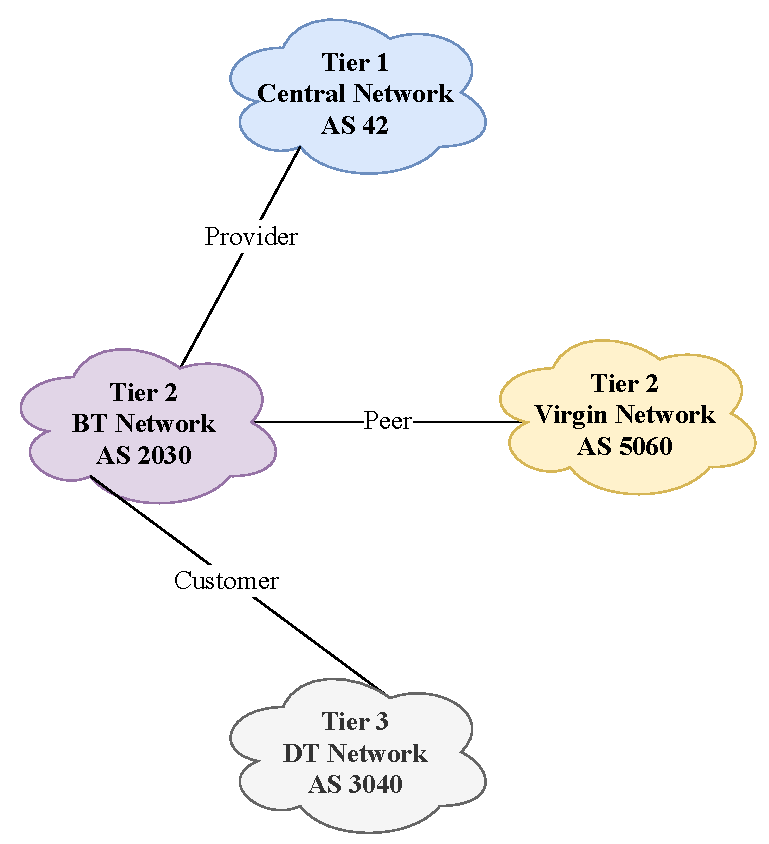
\includegraphics[width=0.5\linewidth]{relationships}
    \caption{Business Relationships of BT Network with Neighbouring ISPs.}
    \label{fig:relationships}
\end{figure*}


\subsection{Provider: Central Network}
Since BT Network is a Tier-2 ISP, it need to be connected to a Tier-1 ISP to gain broader Internet connection. Therefore, BT is connected to Central Network, a Tier-1 ISP, as a customer which makes it a network provider for BT.

\subsection{Peer: Virgin Network}
BT Network forms a Peer relationship with Virgin Network. This allows Virgin Network to connect to BT Network at zero cost and vice versa.

\subsection{Customer: DT Network}
\label{sec:dt}
BT Network forms a Provider-Customer relationship with DT Network, in which BT is the provider and DT is the customer. In other words, DT gains access to the broader Internet through BT at a cost.

\section{Roles of Network Components}
\label{sec:components}

There are 6 physical components in our network in total, of whcih 3 are Cisco routers and the other 3 are TOSHIBA laptops. Each component plays an important role in the network.

\subsection{Routers}
In terms of connection, each router is attached with one customer subnet and thus providing Internet service to one customer. Router 1 (BT-R001) is not physically conncted to any outside network, while Router 2 (BT-R002) is connected to DT Network and Router 3 (BT-R003) is connected to Virgin Network and Central Network through cables.

In terms of routing, all routers are Level-1 routers in intra-domain ISIS routing protocol. In BGP routing protocol, Router 1 (BT-R001) acts as an Internal BGP (IBGP) router while Router 2 (BT-R002) and Router 3 (BT-R003) act as External BGP (EBGP) routers. 



\subsection{Laptops}

All laptops are running a Ubuntu 16.04 system. Each of them is connected to a customer subnet thourgh a cable. 
In terms of services, Laptop 1 (BT001) provides DNS service for \texttt{bt.lboro} as a secondary DNS server and WWW service at \texttt{http://bt.lboro}. It also acts as a secure SSH access point to routers for administrative purposes. 
Laptop 2 (BT002) doesn't provide any service and thus acts act an normal user in the network. 
Laptop 3 (BT003) provides a DNS service for \texttt{bt.lboro} as a primary DNS server. In addition, it provides an Email service at \texttt{bt.lboro}.


\section{Organisation of the Report}
\label{sec:organisation}

The report is organised as follows. We describe the architecture of BT Network on the network layer in Chapter \ref{chap:architecture}. A Network Diagram involving all physical components and connections is drawn in the chapter. Then, IP addresses for interfaces in the network are carefully allocated and configured. 

In order to allow packets to be forwarded within and outside the network, proper intra-domain and inter-domain routing protocols are set up and tested in Chapter \ref{chap:routing}. 

In Chapter \ref{chap:applications}, we move up to the application layer and set up various services in the network as listed in Section \ref{sec:services}.

Main conclusions drawn from the building process and possible further work are discussed in Chapter \ref{chap:discussion}. At last, a summary of contributions for each group member is presented in Chapter \ref{chap:contributions}.

Although the report does not necessarily reflect the actural order of steps in our building process (eg. remote SSH access was set up before BGP), readers can be assured that all results presented can be reproduced by following the natural order of the report.

To ensure readability, rationale behind important decisions made, problems we encountered and their respectively solutions, alternative ways of configurations (if any) as well as reflective commentary for each step of implementation are documented in the report.


\chapter{Network Architecture}
\label{chap:architecture}

\section{Network Diagram}

\subsection{Description}

\subsection{IP Addresses and Interfaces}

\subsection{Connections to Neighbor ISPs}



\section{IP Addresses of Interfaces}

\subsection{Design}

\subsection{Implementation}

\subsection{Evaluation}

\subsection{Commentary}


\section{Network Diagram}
\label{sec:diagram}

\subsection{Description}

A full diagram of BT network is shown in Figure \ref{fig:diagram}.
There are 3 routers in the network, whose names are BT-R001, BT-R002 and BT-R003 resepectively, connected to each other. 
Each connection forms a Router-Router subnet with only 2 interfaces.

On the other hand, each router is connected with a laptop separately named as BT001, BT002 and BT003 and thus forms a Router-Laptop subnet.
A customer of BT Network is assigned with a Router-Laptop subnet and has a minimum of 10 host IP addresses.

To connect to neighbor ISPs, a Router-Neighbor subnet is formed for each connection. Concretely, Router 2 (BT-R002) is connected to one of DT Network's routers while Router 3 (BT-R003) is connected to one of Virgin Network's and Central Network's routers separately.

All of the above connections are through physical cables.

\begin{landscape}
\begin{figure}[t!]
    \centering
    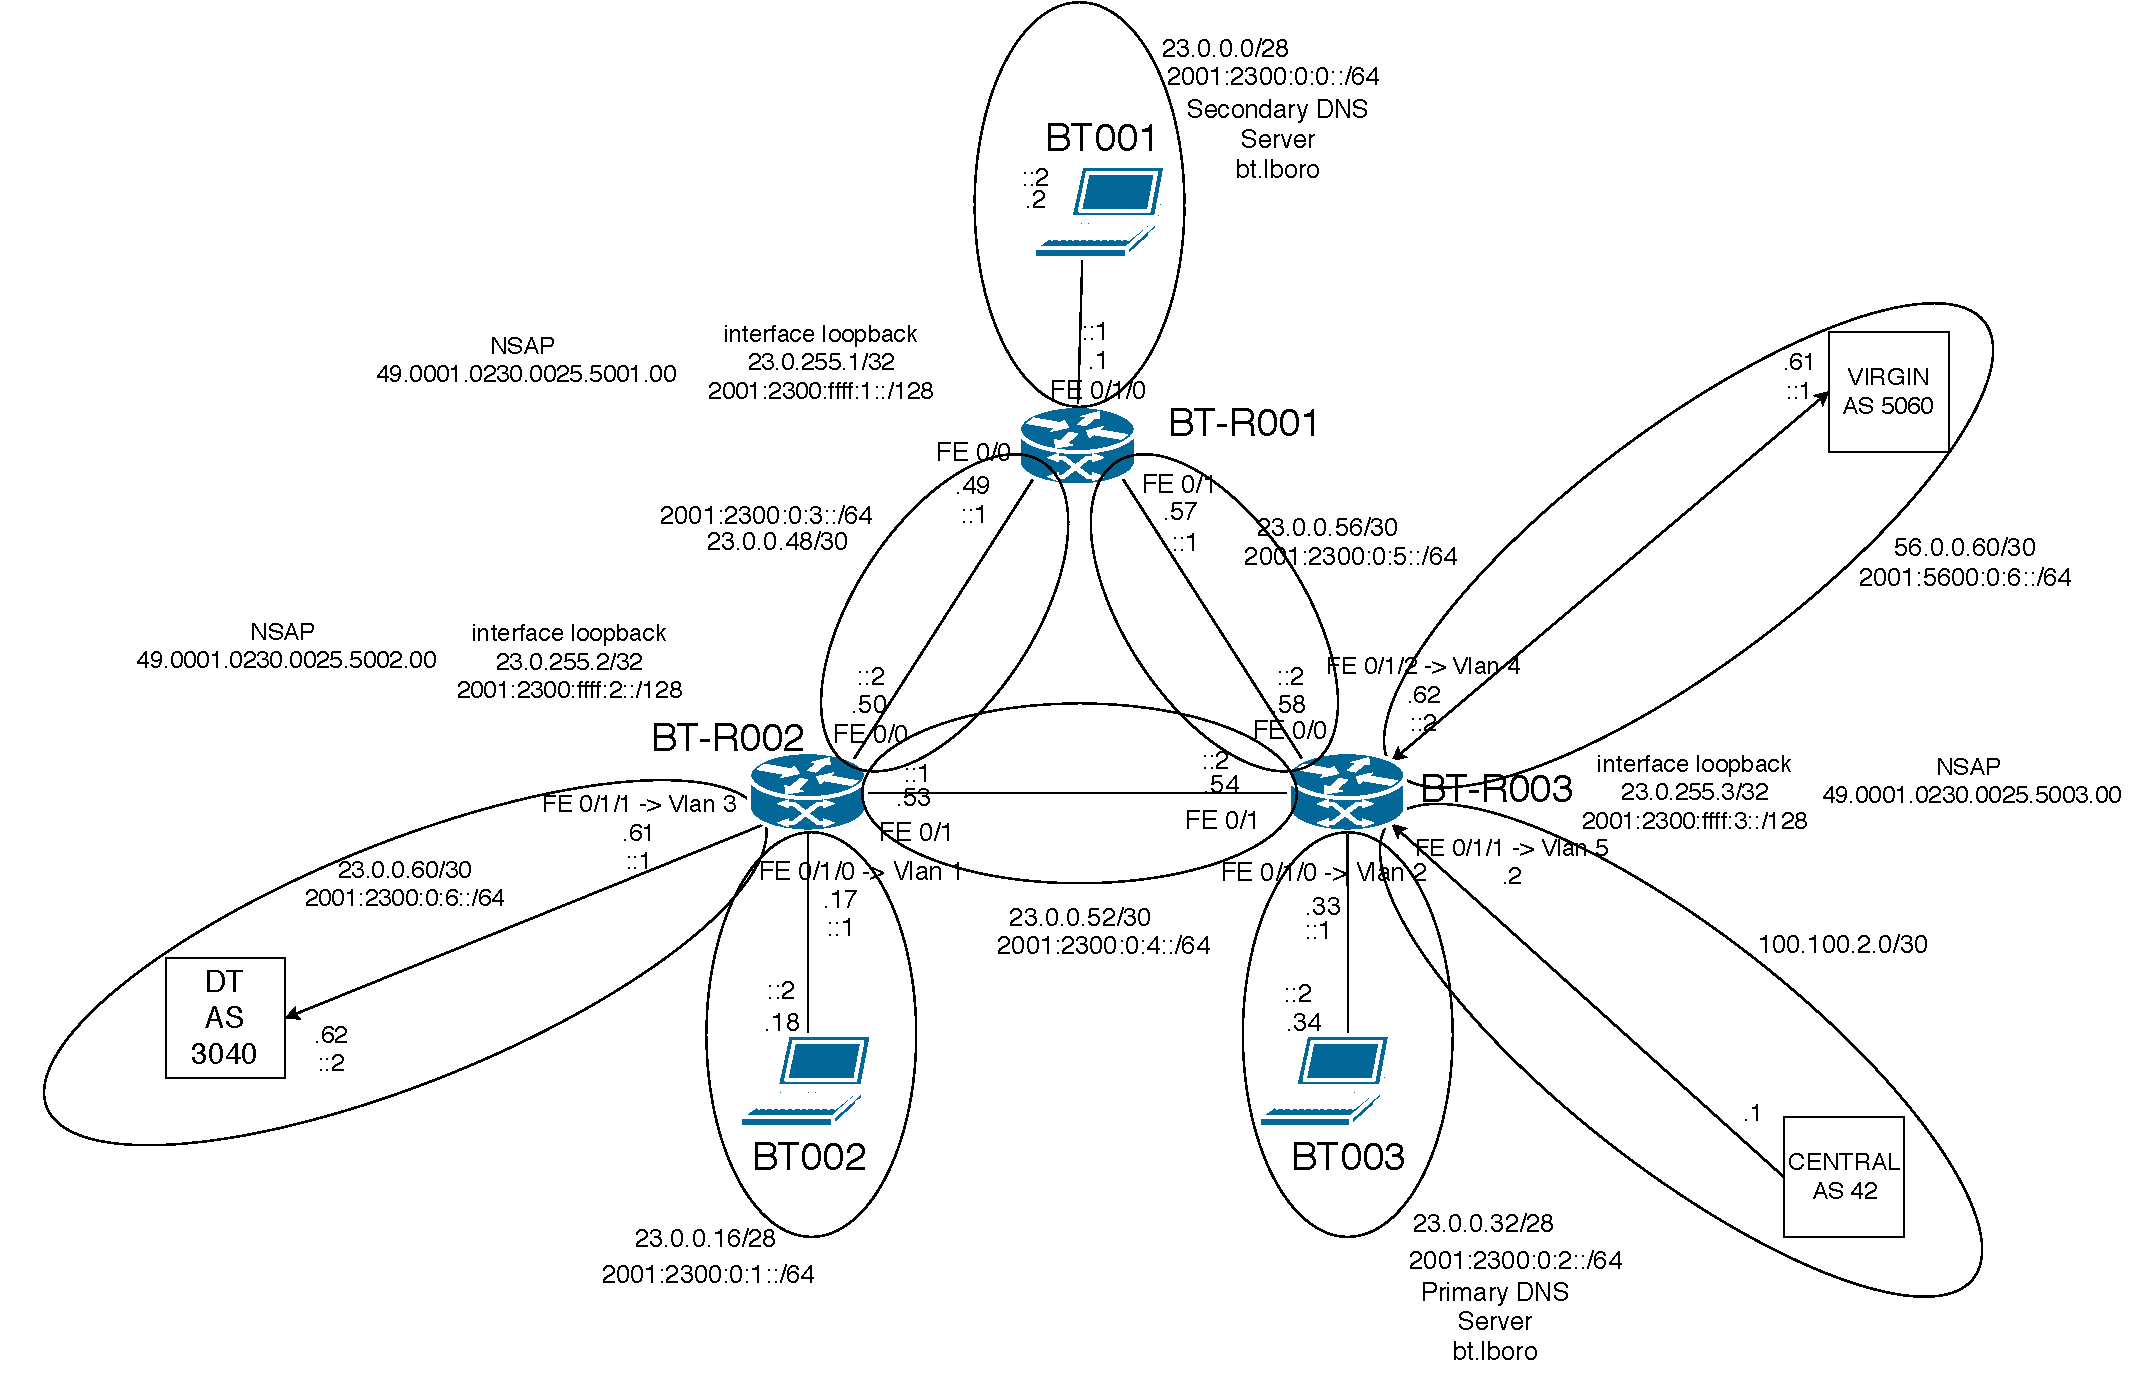
\includegraphics[width=\linewidth]{diagram}
    \caption{Full Network Diagram of BT Network.}
    \label{fig:diagram}
\end{figure}
\end{landscape}




\subsection{IP Addresses and Interfaces}

An IPv4 address range of \texttt{23.0.0.0/8} and IPv6 address range of \texttt{2001:2300::/32} are allocated to BT Network, which are further divided into sub-ranges to be allocated to each subnet.

For IPv4 addressing, a netmask of $n$ is needed for a subnet that demands $X$ host addresses, where $n$ is an integer that satisfies $2^{32-n} - 2 \geq X$ and $n \leq 32$. For our lab, the maximum value for netmask is used in order to minimize the size of each subnet and reserve address space for future customers. However, it's also possible to use a larger value for each Router-Laptop subnet in order to maximize the size of the subnet, given that the number of customers (in this case, $3$) is fixed.

In BT Network, the netmask for each Router-Router and Router-Neighbor subnet is $30$ while the netmask for each Router-Laptop subnet is $28$. In other words, each Router-Router and Router-Neighbor subnet has $2$ guaranteed IPv4 host addresses while each Router-Laptop subnet has $14$ guaranteed IPv4 host addresses. During address block allocation, larger subnet is being considered before smaller one reduce the number of block segments.

For IPv6 addressing, however, each subnet has a fixed netmask of $64$ to ensure that each interface in the subnet has a unique address. The full details of IP address allocation is shown in Table \ref{tab:ip}.

\begin{figure}[ht!]
    \centering
    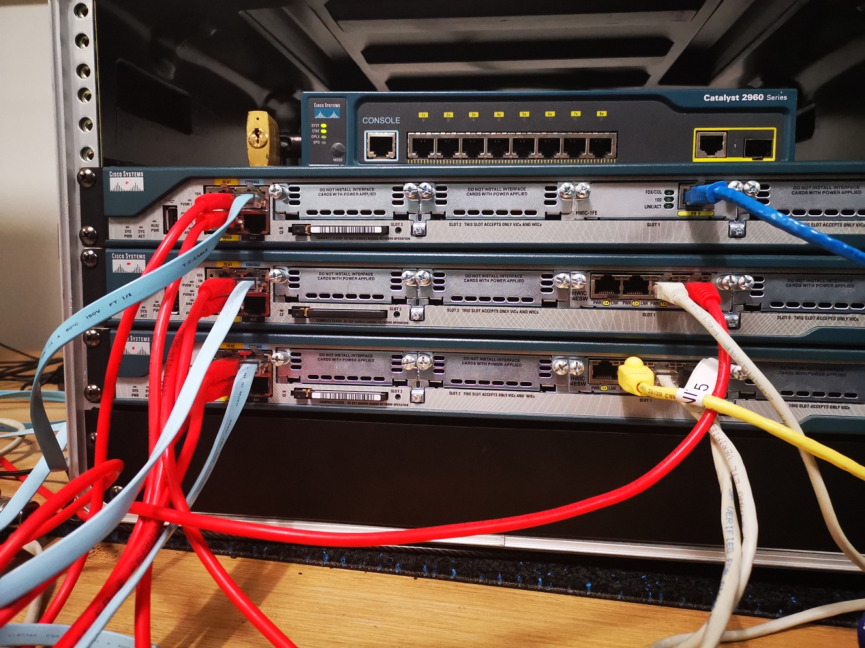
\includegraphics[width=0.8\linewidth]{physical}
    \caption{Physical Connections within BT Network.}
    \label{fig:physical}
\end{figure}

In terms of interfaces, there are $3$ Ethernet interfaces (\texttt{FastEthernet0/0}, \texttt{FastEthernet0/1} and \texttt{FastEthernet0/1/0}) on Router 1, each of which can be assigned with an IP address. On Router 2 and 3, however, there are $6$ Ethernet interfaces each and only $2$ of them (\texttt{FastEthernet0/0} and \texttt{FastEthernet0/1}) can be directly assigned with IP addresses. 
The remaining $4$ interfaces are link layer interfaces and thus does not possess any IP address.
To be assigned with an IP address, such an interface need to be assigned to an Virtual LAN (VLAN) to which the address is actually assigned.

Router-Router connections are established through either \texttt{FastEthernet0/0} or \texttt{FastEthernet0/1} interfaces on both ends while Router-Laptop and Router-Neighbor are through one of the remaining interfaces on the router end.
Since both interfaces are on the left-hand side of each router and such arrangement helps distinguishing between Router-Router connections and others easily as shown in Figure \ref{fig:physical}. Interfaces of both ends for each connection as well as their corresponding IP addresses are detailed in Table \ref{tab:interfaces}.

\begin{landscape}
\scriptsize{
\begin{longtable}[]{@{}lllll@{}}
\toprule
Subnet & IPv4 Address / Netmask & IPv4 Address Range & IPv6
Address / Netmask & IPv6 Address Range\tabularnewline
\midrule
\endhead
\texttt{BT-R001} - \texttt{BT001} & \texttt{23.0.0.0/28} &
\texttt{23.0.0.1} - \texttt{23.0.0.14} & \texttt{2001:2300:0:0::/64} &
\texttt{2001:2300:0:0::1} -
\texttt{2001:2300:0:0:ffff:ffff:ffff:fffe}\tabularnewline
\texttt{BT-R002} - \texttt{BT002} & \texttt{23.0.0.16/28} &
\texttt{23.0.0.17} - \texttt{23.0.0.30} & \texttt{2001:2300:0:1::/64} &
\texttt{2001:2300:0:1::1} -
\texttt{2001:2300:0:1:ffff:ffff:ffff:fffe}\tabularnewline
\texttt{BT-R003} - \texttt{BT003} & \texttt{23.0.0.32/28} &
\texttt{23.0.0.33} - \texttt{23.0.0.62} & \texttt{2001:2300:0:2::/64} &
\texttt{2001:2300:0:2::1} -
\texttt{2001:2300:0:2:ffff:ffff:ffff:fffe}\tabularnewline
\texttt{BT-R001} - \texttt{BT-R002} & \texttt{23.0.0.48/30} &
\texttt{23.0.0.49} - \texttt{23.0.0.50} & \texttt{2001:2300:0:3::/64} &
\texttt{2001:2300:0:3::1} -
\texttt{2001:2300:0:3:ffff:ffff:ffff:fffe}\tabularnewline
\texttt{BT-R002} - \texttt{BT-R003} & \texttt{23.0.0.52/30} &
\texttt{23.0.0.53} - \texttt{23.0.0.54} & \texttt{2001:2300:0:4::/64} &
\texttt{2001:2300:0:4::1} -
\texttt{2001:2300:0:4:ffff:ffff:ffff:fffe}\tabularnewline
\texttt{BT-R001} - \texttt{BT-R003} & \texttt{23.0.0.56/30} &
\texttt{23.0.0.57} - \texttt{23.0.0.58} & \texttt{2001:2300:0:5::/64} &
\texttt{2001:2300:0:5::1} -
\texttt{2001:2300:0:5:ffff:ffff:ffff:fffe}\tabularnewline
\texttt{BT-R002} - \texttt{DT} & \texttt{23.0.0.60/30} &
\texttt{23.0.0.61} - \texttt{23.0.0.62} & \texttt{2001:2300:0:6::/64} &
\texttt{2001:2300:0:6::1} -
\texttt{2001:2300:0:6:ffff:ffff:ffff:fffe}\tabularnewline
\texttt{BT-R003} - \texttt{Virgin} & \texttt{56.0.0.60/30} &
\texttt{56.0.0.61} - \texttt{56.0.0.62} & \texttt{2001:5600:0:6::/64} &
\texttt{2001:5600:0:6::1} -
\texttt{2001:5600:0:6:ffff:ffff:ffff:fffe}\tabularnewline
\texttt{BT-R003} - \texttt{Central} & \texttt{100.100.2.0/30} &
\texttt{100.100.2.1} - \texttt{100.100.2.2} & &\tabularnewline
\bottomrule
\caption{Allocation of IPv4 and IPv6 Addresses to Subnets in BT Network.}
\label{tab:ip}
\end{longtable}
}

\scriptsize{
\begin{longtable}[]{@{}lllllll@{}}
\toprule
Connection & Interface 1 & IPv4 Address & IPv6 Address & Interface 2 & IPv4 Address & IPv6
Address \tabularnewline
\midrule
\endhead
\texttt{BT-R001} - \texttt{BT001} & \texttt{BT-R001}:
\texttt{FastEthernet0/1/0} & \texttt{23.0.0.1} &
\texttt{2001:2300:0:0::1} & \texttt{BT001}: \texttt{eth0} &
\texttt{23.0.0.2} & \texttt{2001:2300:0:0::2}\tabularnewline
\texttt{BT-R002} - \texttt{BT002} & \texttt{BT-R002}:
\texttt{FastEthernet0/1/0} -\textgreater{} \texttt{Vlan\ 1} &
\texttt{23.0.0.17} & \texttt{2001:2300:0:1::1} & \texttt{BT002}:
\texttt{eth0} & \texttt{23.0.0.18} &
\texttt{2001:2300:0:1::2}\tabularnewline
\texttt{BT-R003} - \texttt{BT003} & \texttt{BT-R003}:
\texttt{FastEthernet0/1/0} -\textgreater{} \texttt{Vlan\ 2} &
\texttt{23.0.0.33} & \texttt{2001:2300:0:2::1} & \texttt{BT003}:
\texttt{eth0} & \texttt{23.0.0.34} &
\texttt{2001:2300:0:2::2}\tabularnewline
\texttt{BT-R001} - \texttt{BT-R002} & \texttt{BT-R001}:
\texttt{FastEthernet0/0} & \texttt{23.0.0.49} &
\texttt{2001:2300:0:3::1} & \texttt{BT-R002}: \texttt{FastEthernet0/0} &
\texttt{23.0.0.50} & \texttt{2001:2300:0:3::2}\tabularnewline
\texttt{BT-R002} - \texttt{BT-R003} & \texttt{BT-R002}:
\texttt{FastEthernet0/1} & \texttt{23.0.0.53} &
\texttt{2001:2300:0:4::1} & \texttt{BT-R003}: \texttt{FastEthernet0/1} &
\texttt{23.0.0.54} & \texttt{2001:2300:0:4::2}\tabularnewline
\texttt{BT-R001} - \texttt{BT-R003} & \texttt{BT-R001}:
\texttt{FastEthernet0/1} & \texttt{23.0.0.57} &
\texttt{2001:2300:0:5::1} & \texttt{BT-R003}: \texttt{FastEthernet0/0} &
\texttt{23.0.0.58} & \texttt{2001:2300:0:5::2}\tabularnewline
\texttt{BT-R002} - \texttt{DT} & \texttt{BT-R002}:
\texttt{FastEthernet0/1/1} -\textgreater{} \texttt{Vlan\ 3} &
\texttt{23.0.0.61} & \texttt{2001:2300:0:6::1} & \texttt{DT} &
\texttt{23.0.0.62} & \texttt{2001:2300:0:6::2}\tabularnewline
\texttt{BT-R003} - \texttt{Virgin} & \texttt{BT-R003}:
\texttt{FastEthernet0/1/2} -\textgreater{} \texttt{Vlan\ 4} &
\texttt{56.0.0.62} & \texttt{2001:5600:0:6::2} & \texttt{Virgin} &
\texttt{56.0.0.61} & \texttt{2001:5600:0:6::1}\tabularnewline
\texttt{BT-R003} - \texttt{Central} & \texttt{BT-R003}:
\texttt{FastEthernet0/1/1} -\textgreater{} \texttt{Vlan\ 5} &
\texttt{100.100.2.2} & & \texttt{Central} & \texttt{100.100.2.1}
&\tabularnewline
\bottomrule
\caption{Interfaces for Each Physical Connection and Corresponding IPv4 and IPv6 Addresses.}
\label{tab:interfaces}
\end{longtable}
}

\end{landscape}







\newpage
\section{IP Addresses of Interfaces}
\label{sec:IP}

% \subsection{Design}

Assigning IP addresses\citep{rfc791}\citep{rfc2460} to interfaces should be the first step in building BT Network since all network services listed in \ref{sec:services} cannot operate without IP addresses.
The assignment of IP addresses in Table \ref{tab:ip} and \ref{tab:interfaces} is implemented.

\subsection{Implementation}

\subsubsection{Routers}

For Router 1 (BT-R001), IP addresses are assigned directly to physical interfaces as all interfaces are network layer interfaces.

\begin{lstlisting}
int fa0/0
ip address 23.0.0.49 255.255.255.252
ipv6 address 2001:2300:0:3::1/64
no shutdown

int fa0/1
ip address 23.0.0.57 255.255.255.252
ipv6 address 2001:2300:0:5::1/64
no shutdown

int fa0/1/0
ip address 23.0.0.1 255.255.255.240
ipv6 address 2001:2300:0:0::1/64
no shutdown
\end{lstlisting}

For Router 2 (BT-R002), however, only $2$ interfaces (\texttt{FastEhternet0/0} and \texttt{FastEhternet0/1}) each are network layer interfaces. The remaining $4$ interfaces are link layer interfaces and need to be assigned to an VLAN separately se where an IP address can be assigned. 

\begin{lstlisting}
int fa0/0
ip address 23.0.0.50 255.255.255.252
ipv6 address 2001:2300:0:3::2/64
no shutdown

int fa0/1
ip address 23.0.0.53 255.255.255.252
ipv6 address 2001:2300:0:4::1/64
no shutdown

vlan 1
int fa0/1/0
switchport mode access
switchport access vlan 1
int vlan 1
ip address 23.0.0.17 255.255.255.240
ipv6 address 2001:2300:0:1::1/64
no shutdown

vlan 3
int fa0/1/1
switchport mode access
switchport access vlan 3
int vlan 3
ip address 23.0.0.61 255.255.255.252
ipv6 address 2001:2300:0:6::1/64
no shutdown
\end{lstlisting}

Similarly, IP addresses are assigned to Router 3 (BT-R003).

\begin{lstlisting}
int fa0/0
ip address 23.0.0.58 255.255.255.252
ipv6 address 2001:2300:0:5::2/64
no shutdown

int fa0/1
ip address 23.0.0.54 255.255.255.252
ipv6 address 2001:2300:4::2/64
no shutdown

vlan 2
int fa0/1/0
switchport mode access
switchport access vlan 2
int vlan 2
ip address 23.0.0.33 255.255.255.240
ipv6 address 2001:2300:0:2::1/64
no shutdown

vlan 4
int fa0/1/2
switchport mode access
switchport access vlan 4
int vlan 4
ip address 56.0.0.62 255.255.255.252
ipv6 address 2001:5600:0:6::2/64
no shutdown

vlan 5
int fa0/1/1
switchport mode access
switchport access vlan 5
int vlan 5
ip address 100.100.2.2 255.255.255.252
no shutdown
\end{lstlisting}

\subsubsection{Laptops}

Unlike routers, the IP assignment of laptops' interfaces are more aligned since all laptops are of the same model. 
On Laptop 1 (BT001), the file \texttt{/etc/network/interface} is edited as follows before rebooting to apply changes. 
Similarly, IP address can are assigned to Laptop 2's (BT002) and Laptop 3's (BT003) interfaces respectively. 
Full configuration for all laptops are detailed in Appendix \ref{app:laptops}.

\begin{lstlisting}[language=sh]
auto lo
iface lo inet loopback
auto eth0
ifacce eth0 inet static 
address 23.0.0.2
netmask 255.255.255.240
gateway 23.0.0.1

ifacce eth0 inet6 static 
address 2001:2300::2
netmask 64
gateway 2001:2300::1
\end{lstlisting}

\subsection{Evaluation}

On all $3$ routers, the implementation of IP assignments is evaluated using \texttt{show ip int brief} and \texttt{show ipv6 int brief}. These $2$ commands show IPv4 and IPv6 addresses of interfaces on routers respectively.
Sucessful assignment of IP addresses to routers' interfaces is evident from Figure \ref{fig:ipv4-router} and \ref{fig:ipv6-router}.

\begin{figure*}[ht!]
    \centering
    \begin{subfigure}[b]{0.67\textwidth}
        \centering
        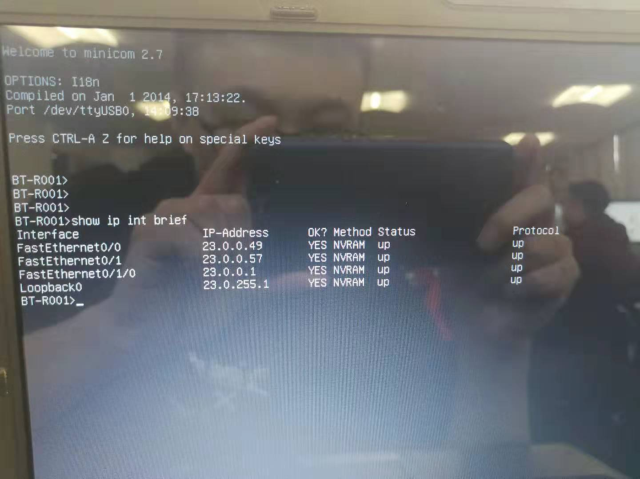
\includegraphics[width=\linewidth]{ipv4-router1}
        \caption{Router 1 (BT-R001)}
    \end{subfigure}
    \hfill
    \begin{minipage}[b]{0.3\textwidth}
	    \begin{subfigure}[b]{\linewidth}
	        \centering
	        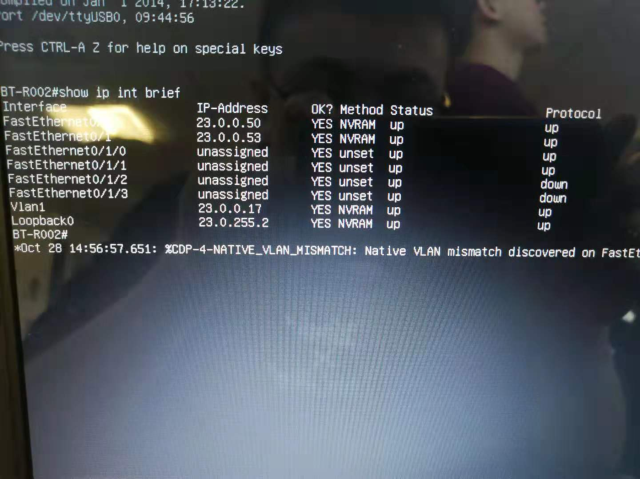
\includegraphics[width=\linewidth]{ipv4-router2}
	        \caption{Router 2 (BT-R002)}
	    \end{subfigure}
	    \\
	    \begin{subfigure}[b]{\linewidth}
	        \centering
	        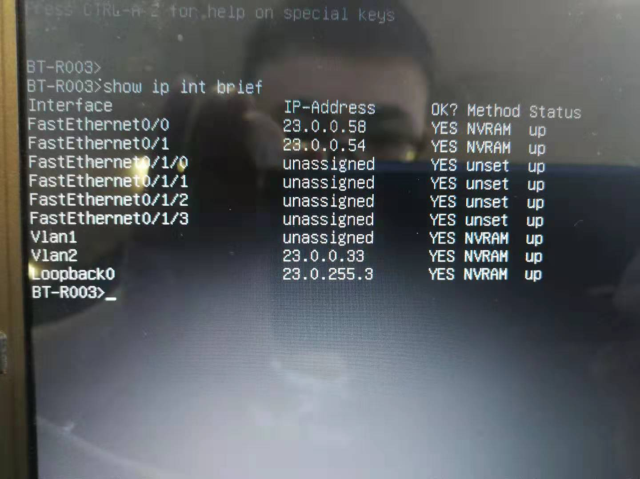
\includegraphics[width=\linewidth]{ipv4-router3}
	        \caption{Router 3 (BT-R003)}
	    \end{subfigure}
	\end{minipage}
    \caption{Sucessful Assignment of IPv4 Addresses to Routers' Interfaces.}
    \label{fig:ipv4-router}
\end{figure*}

\begin{figure*}[ht!]
    \centering
    \begin{subfigure}[b]{0.67\textwidth}
        \centering
        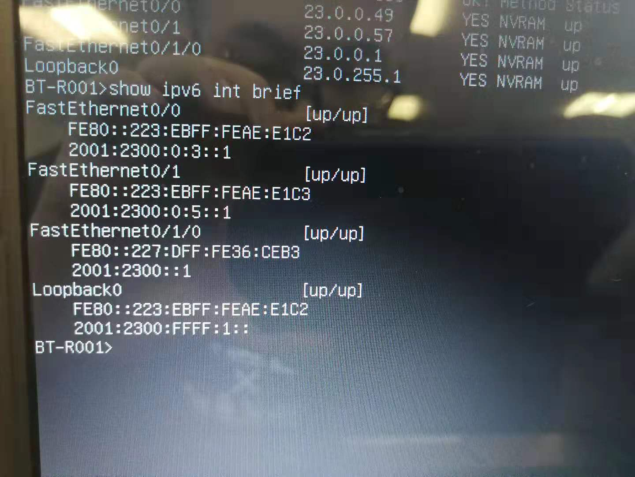
\includegraphics[width=\linewidth]{ipv6-router1}
        \caption{Router 1 (BT-R001)}
    \end{subfigure}
    \hfill
    \begin{minipage}[b]{0.3\textwidth}
	    \begin{subfigure}[b]{\linewidth}
	        \centering
	        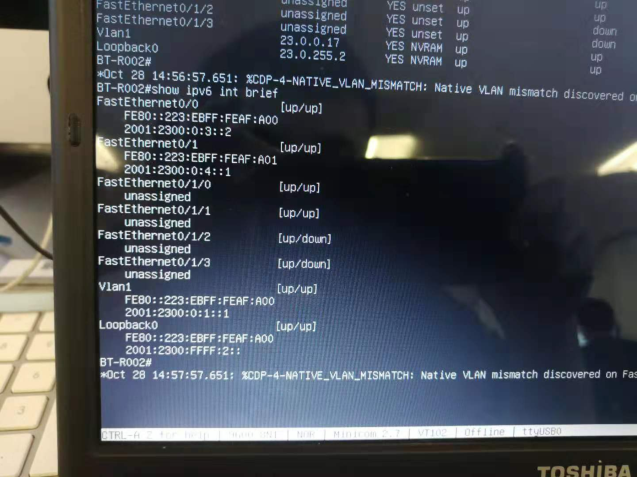
\includegraphics[width=\linewidth]{ipv6-router2}
	        \caption{Router 2 (BT-R002)}
	    \end{subfigure}
	    \\
	    \begin{subfigure}[b]{\linewidth}
	        \centering
	        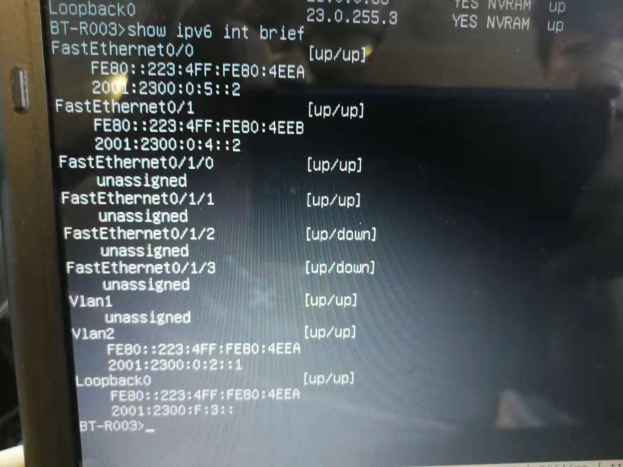
\includegraphics[width=\linewidth]{ipv6-router3}
	        \caption{Router 3 (BT-R003)}
	    \end{subfigure}
	\end{minipage}
    \caption{Sucessful Assignment of IPv6 Addresses to Routers' Interfaces.}
    \label{fig:ipv6-router}
\end{figure*}


On the laptops' side, the implementation of IP assignments is evaluated using \texttt{ifconfig} command.
Sucessful assignment of IP addresses to laptops' interfaces is evident from Figure \ref{fig:ip-laptop}.

\begin{figure*}[ht!]
    \centering
    \begin{subfigure}[b]{0.67\textwidth}
        \centering
        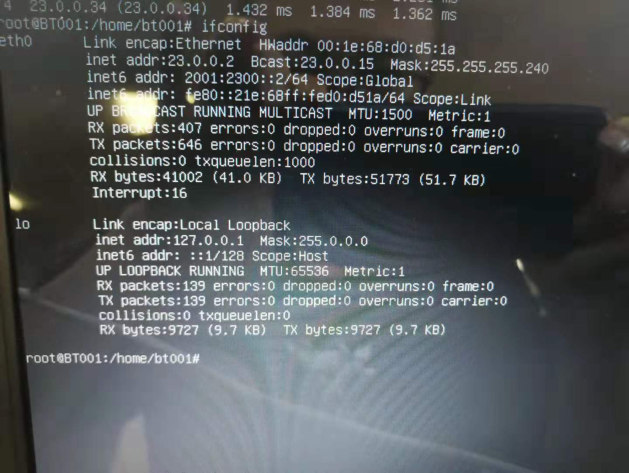
\includegraphics[width=\linewidth]{ip-laptop1}
        \caption{Laptop 1 (BT001)}
    \end{subfigure}
    \hfill
    \begin{minipage}[b]{0.3\textwidth}
	    \begin{subfigure}[b]{\linewidth}
	        \centering
	        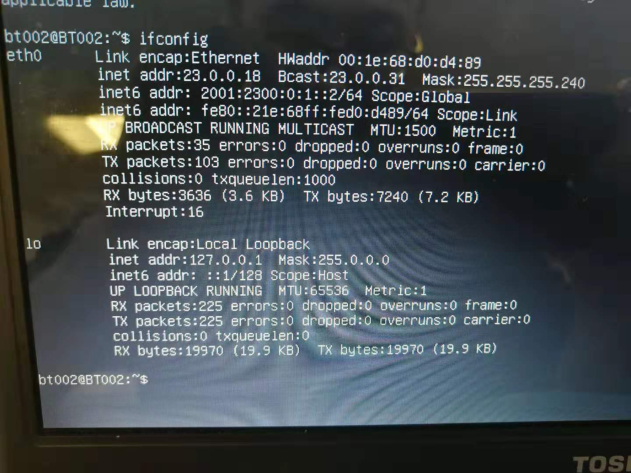
\includegraphics[width=\linewidth]{ip-laptop2}
	        \caption{Laptop 2 (BT002)}
	    \end{subfigure}
	    \\
	    \begin{subfigure}[b]{\linewidth}
	        \centering
	        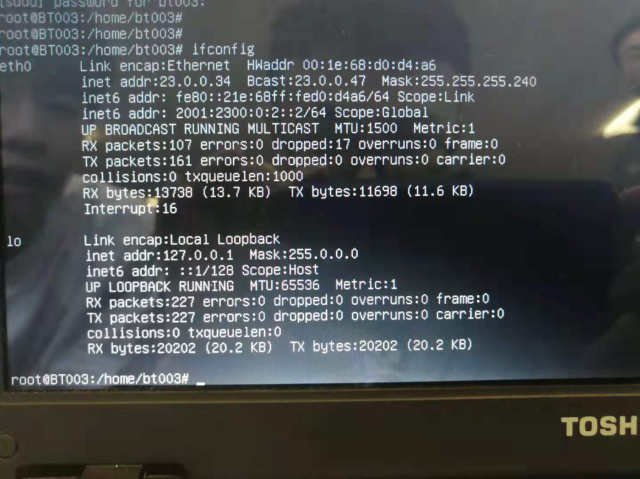
\includegraphics[width=\linewidth]{ip-laptop3}
	        \caption{Laptop 3 (BT003)}
	    \end{subfigure}
	\end{minipage}
    \caption{Sucessful Assignment of IPv4 and IPv6 Addresses to Laptops' Interfaces.}
    \label{fig:ip-laptop}
\end{figure*}

% \subsection{Commentary}


\newpage


\chapter{Routing Protocols in the Network}
\label{chap:routing}




\section{Intra-domain Routing Protocol: IS-IS}
\label{sec:isis}

\subsection{Design}

Due to the limitation of the static routing, routers cannot find alternative paths if a set path is broken and thus a new path need to be set manually. 
In contrast, dynamic routing always finds the least cost path even when the previous least cost path is broken.
Popular dynamic routing protocols include distance vector based protocols like Routing Information Protocol (RIP)\citep{rfc2453} and link state based protocols like Intermediate System to Intermediate System (IS-IS)\citep{rfc1142} and Open Shortest Path First (OSPF)\citep{rfc2328}. 

In this lab, the IS-IS is used as the Interior Gateway Protocol (IGP), which provides faster convergence and larger scalability compared to distance vector based protocols. 
IS-IS is short for Intermediate System to Intermediate System Routing Protocol.
By using this protocol, each router maintains a database which has a map of the whole topology and all routers have the same information. The best path to every destination is computed by all routers. 
Figure \ref{fig:isis} shows the design of IS-IS protocol in BT Network. As the figure shows, the network only has level-1 routers for internal routing.

\begin{figure}[ht!]
    \centering
    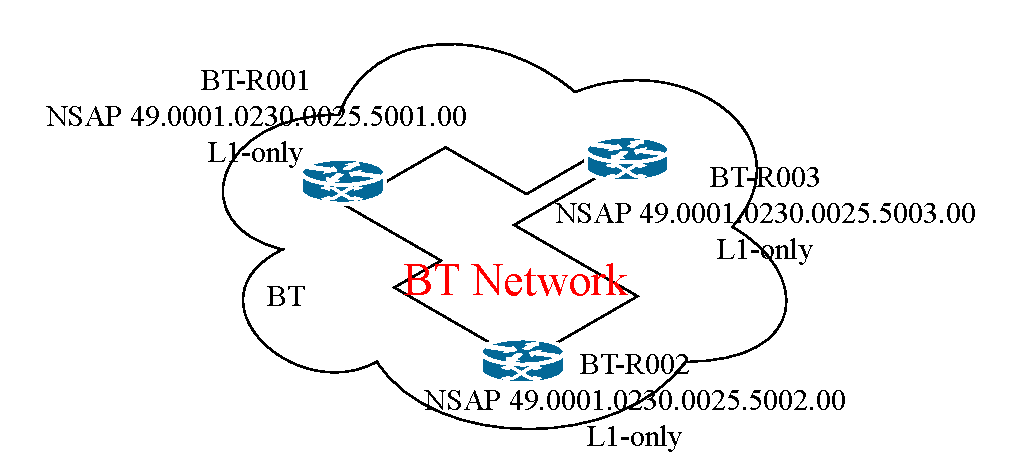
\includegraphics[width=\linewidth]{isis}
    \caption{Design of IS-IS Protocol in BT Network.}
    \label{fig:isis}
\end{figure}

\subsection{Loopback Addresses and NSAP for Routers}

To set up IS-IS, an unique loopback address is needed for each router. 
An IPv4 address block of \texttt{23.0.255.0/24} and IPv6 address block of \texttt{2001:2300:ffff::/48} is allocated for loopback addresses. 

Following the CLNS addressing convention, each router is then assigned with a NSAP. A NSAP has $3$ main components. 

According to the convention, the leading Area ID is composed of AFI ($49$) and Area Address ($0001$). 
The System ID followed is set to the IPv4 loopback address of the router. If the loopback address is $ABC.DEF.GHI.JKL$, then System ID should be $ABCD.EFGH.IJKL$.
The last main component is N-Selector (NSEL) and set to $00$.

The assignment of addresses and NSAP to routers are detailed in Table \ref{tab:isis}.

\begin{longtable}[]{@{}llll@{}}
\toprule
Router & IPv4 Loopback Address & IPv6 Loopback Address & NSAP\tabularnewline
\midrule
\endhead
BT-R001 & 23.0.255.1 & 2001:2300:ffff:1:: & 49.0001.0230.0025.5001.00\tabularnewline
BT-R002 & 23.0.255.2 & 2001:2300:ffff:2:: & 49.0001.0230.0025.5002.00\tabularnewline
BT-R003 & 23.0.255.3 & 2001:2300:ffff:3:: & 49.0001.0230.0025.5003.00\tabularnewline
\bottomrule
\caption{IP Loopback Addresses and NSAP for Routers in BT Network.}
\label{tab:isis}
\end{longtable}



\subsection{Implementation}

IS-IS is set up on Router 1 (BT-R001) using the following commands.

\begin{lstlisting}
interface Loopback0
ip address 23.0.255.1 255.255.255.255
ipv6 address 2001:2300:FFFF:1::/128

router isis
net 49.0001.0230.0025.5001.00
is-type level-1
\end{lstlisting}

Then, IS-IS is turned on on all interfaces to internal routers.

\begin{lstlisting}
interface FastEthernet0/0
ip router isis
ipv6 router isis

interface FastEthernet0/1
ip router isis
ipv6 router isis

interface FastEthernet0/1/0
ip router isis
ipv6 router isis
\end{lstlisting}

\clearpage

However, IS-IS routes should not be broadcasted nor received through the loopback interface (\texttt{Loopback0}) while the route to corresponding subnet should be broadcasted to other internal routers. Therefore, the loopback interface should be a passive interface in IS-IS protocol.

\begin{lstlisting}
router isis
passive-interface Loopback0
\end{lstlisting}

For Router 2 (BT-R002) and Router 3 (BT-R002), IS-IS is set up similarly using the above commands. The main difference is that interfaces to external routers (VLAN 3 for Router 2 and VLAN 4 \& 5 for Router 3) should be passive interfaces as well. Below is the configuration for Router 2.

\begin{lstlisting}
interface Loopback0
ip address 23.0.255.2 255.255.255.255
ipv6 address 2001:2300:FFFF:2::/128

router isis
net 49.0001.0230.0025.5002.00
is-type level-1
passive-interface Vlan3
passive-interface Loopback0

interface FastEthernet0/0
ip router isis
ipv6 router isis

interface FastEthernet0/1
ip router isis
ipv6 router isis

interface Vlan1
ip router isis
ipv6 router isis
\end{lstlisting}

Below is the configuration for Router 3.

\begin{lstlisting}
interface Loopback0
ip address 23.0.255.3 255.255.255.255
ipv6 address 2001:2300:FFFF:3::/128

router isis
net 49.0001.0230.0025.5003.00
is-type level-1
passive-interface Vlan4
passive-interface Vlan5
passive-interface Loopback0

interface FastEthernet0/0
ip router isis
ipv6 router isis

interface FastEthernet0/1
ip router isis
ipv6 router isis

interface Vlan2
ip router isis
ipv6 router isis
\end{lstlisting}


\subsection{Evaluation}

Once the IS-IS is set up, use \texttt{traceroute} command to check the IPv4 path from Laptop 1 (BT001, IPv4 Address: \texttt{23.0.0.2}) to Laptop 2 (BT002, IPv4 Address: \texttt{23.0.0.18}) in the network.

\begin{lstlisting}[language=sh]
traceroute 23.0.0.34
\end{lstlisting}

Figure \ref{fig:isis-traceroute} shows the route taken is 
\texttt{Laptop 1 (BT001, IPv4 Address: 23.0.0.2)
-> Router 1 (BT-R001, IPv4 Address: 23.0.0.1) 
-> Router 2 (BT-R002, IPv4 Address: 23.0.0.50)
-> Laptop 2 (BT002, IPv4 Address: 23.0.0.18)}, which is a correct route.
Routes from Laptop 1 to Laptop 3 as well as from Laptop 2 to Laptop 3 are tested and shown in the figure as well.

\begin{figure}[ht!]
    \centering
    \begin{subfigure}[b]{\textwidth}
        \centering
        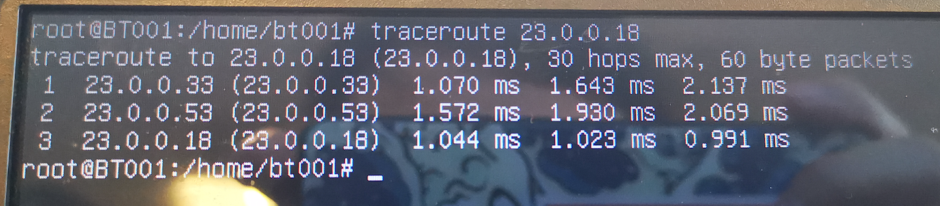
\includegraphics[width=\linewidth]{isis-traceroute-1-2}
        \caption{\texttt{traceroute} from Laptop 1 (BT001) to Laptop 2 (BT002)}
    \end{subfigure}
    ~
    \begin{subfigure}[b]{\textwidth}
        \centering
        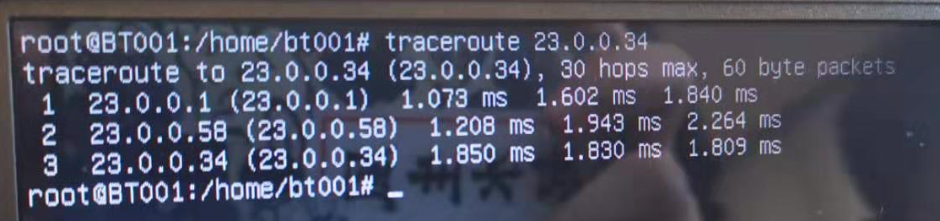
\includegraphics[width=\linewidth]{isis-traceroute-1-3}
        \caption{\texttt{traceroute} from Laptop 1 (BT001) to Laptop 3 (BT003)}
    \end{subfigure}
    ~
    \begin{subfigure}[b]{\textwidth}
        \centering
        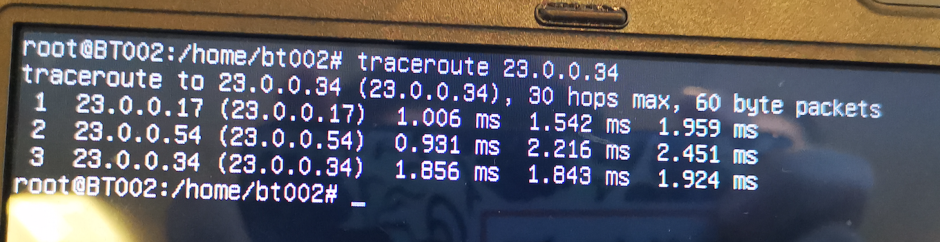
\includegraphics[width=\linewidth]{isis-traceroute-2-3}
        \caption{\texttt{traceroute} from Laptop 2 (BT002) to Laptop 3 (BT003)}
    \end{subfigure}
    \caption{Tracing IPv4 Routes between Laptops using \texttt{traceroute}.}
    \label{fig:isis-traceroute}
\end{figure}

Similiar results can be observed for IPv6 routes in Figure \ref{fig:isis-traceroute-ipv6}. The IPv6 Route taken from Laptop 1 to Laptop 2 is 
\texttt{Laptop 1 (BT001, IPv6 Address: 2001:2300::2)
-> Router 1 (BT-R001, IPv6 Address: 2001:2300::1) 
-> Router 2 (BT-R002, IPv6 Address: 2001:2300:3:2::2)
-> Laptop 2 (BT002, IPv6 Address: 2001:2300:0:1::2)}, , which is also a correct route.
Routes from Laptop 1 to Laptop 3 as well as from Laptop 2 to Laptop 3 are tested and shown in the figure as well.


\begin{figure}[ht!]
    \centering
    \begin{subfigure}[b]{\textwidth}
        \centering
        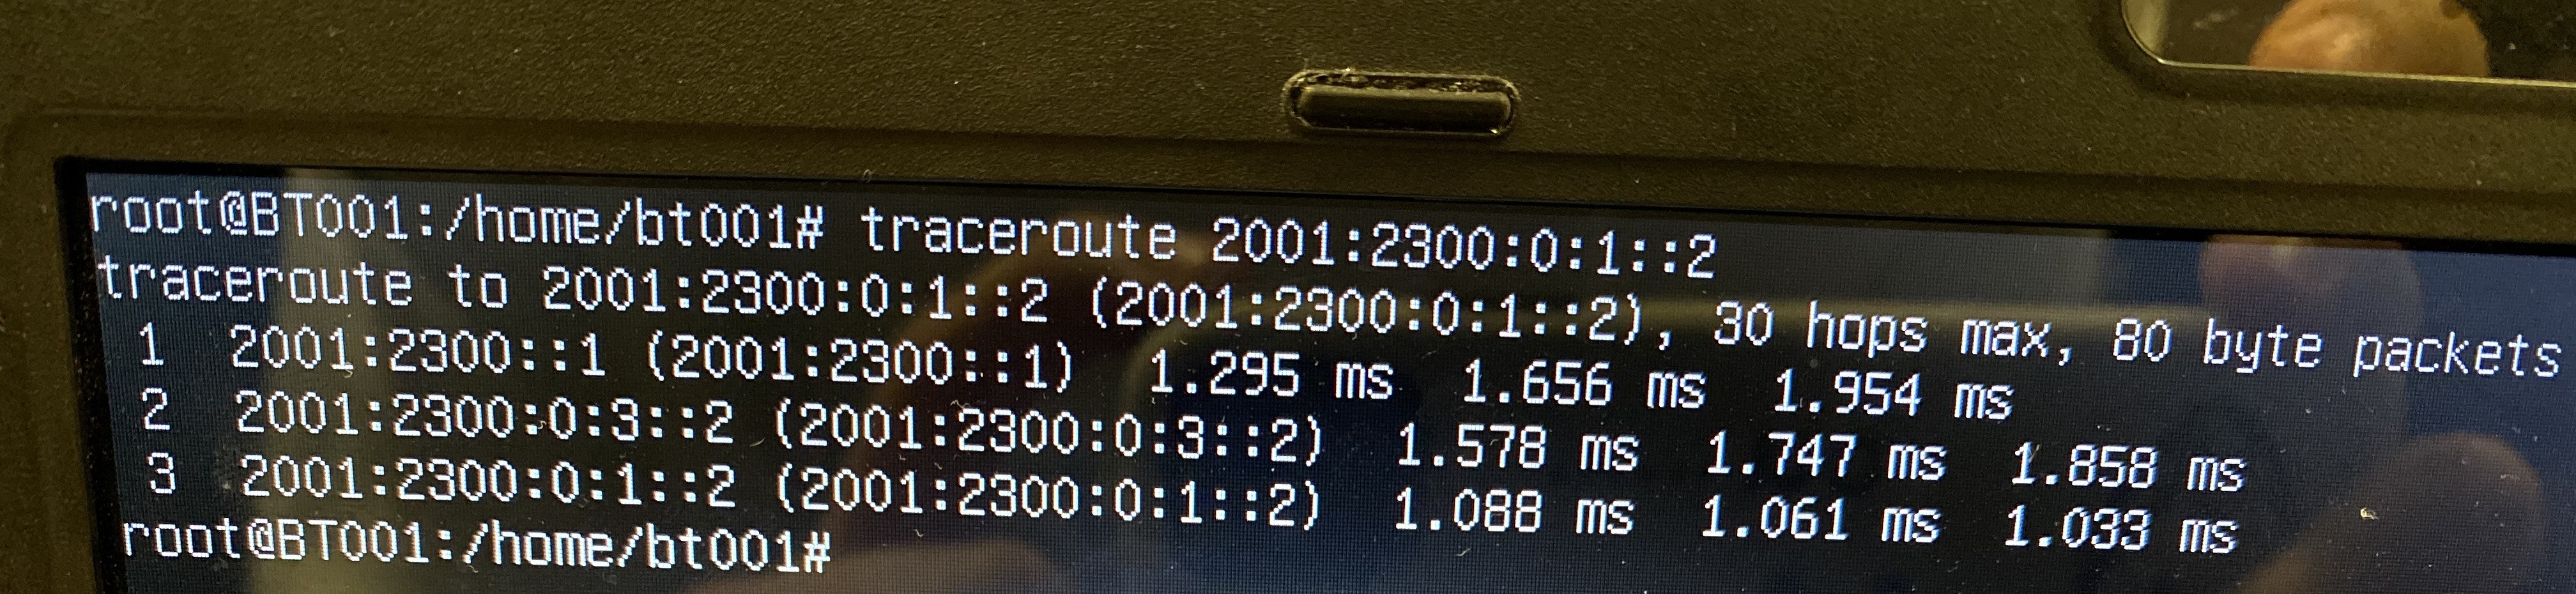
\includegraphics[width=\linewidth]{isis-traceroute-ipv6-1-2}
        \caption{\texttt{traceroute} from Laptop 1 (BT001) to Laptop 2 (BT002)}
    \end{subfigure}
    ~
    \begin{subfigure}[b]{\textwidth}
        \centering
        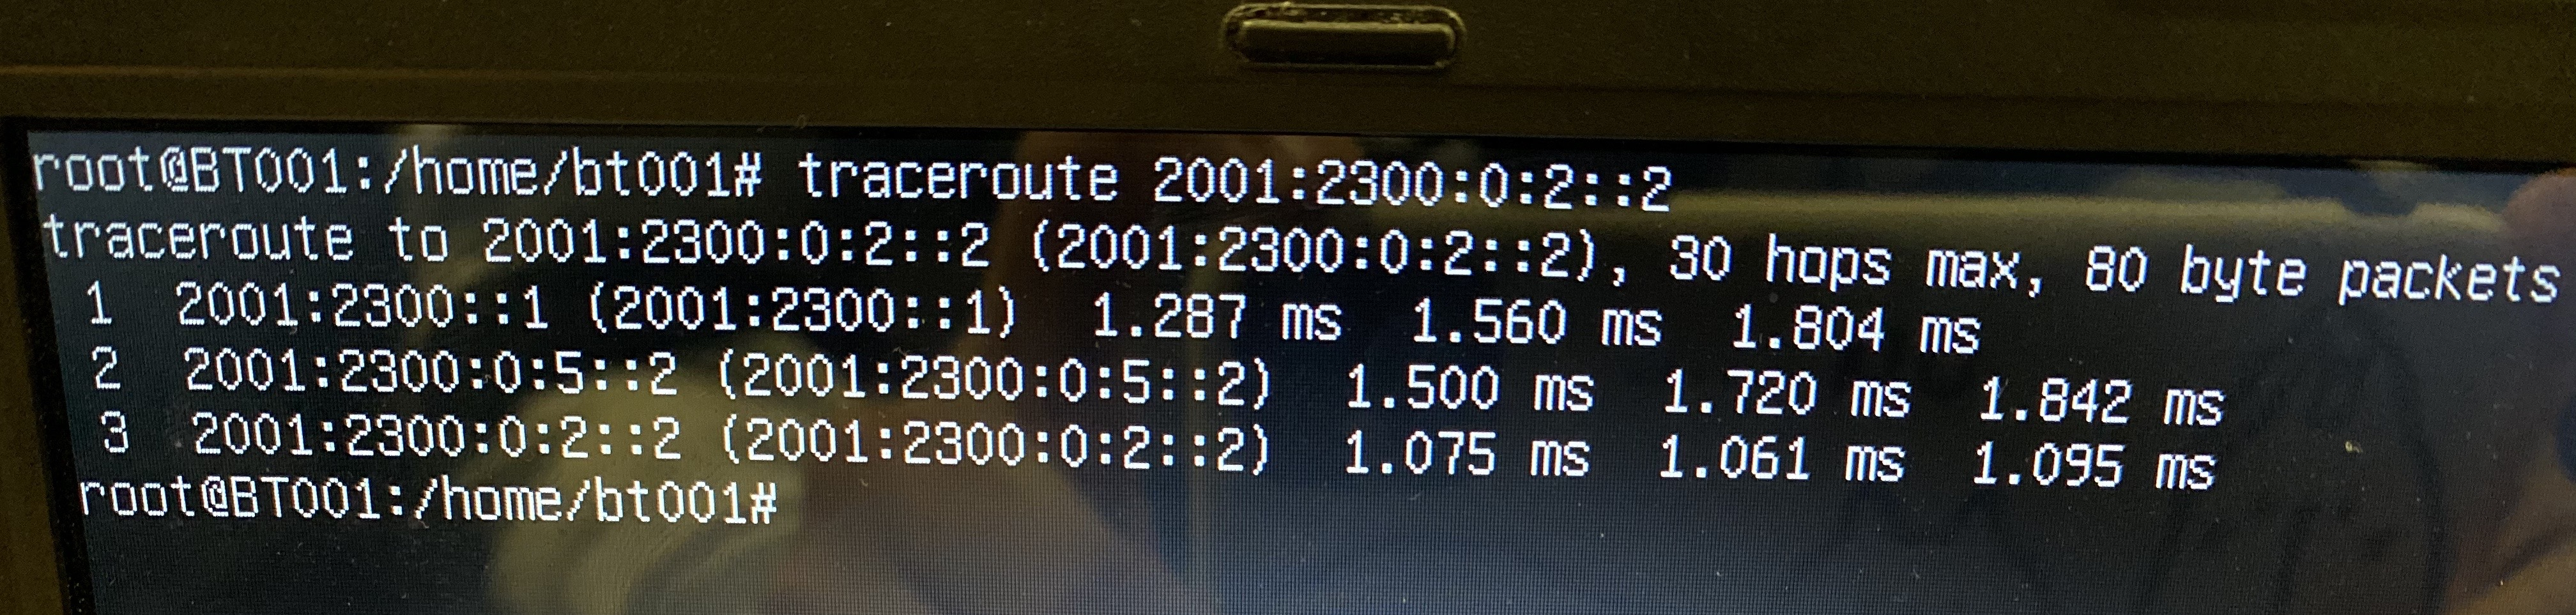
\includegraphics[width=\linewidth]{isis-traceroute-ipv6-1-3}
        \caption{\texttt{traceroute} from Laptop 1 (BT001) to Laptop 3 (BT003)}
    \end{subfigure}
    ~
    \begin{subfigure}[b]{\textwidth}
        \centering
        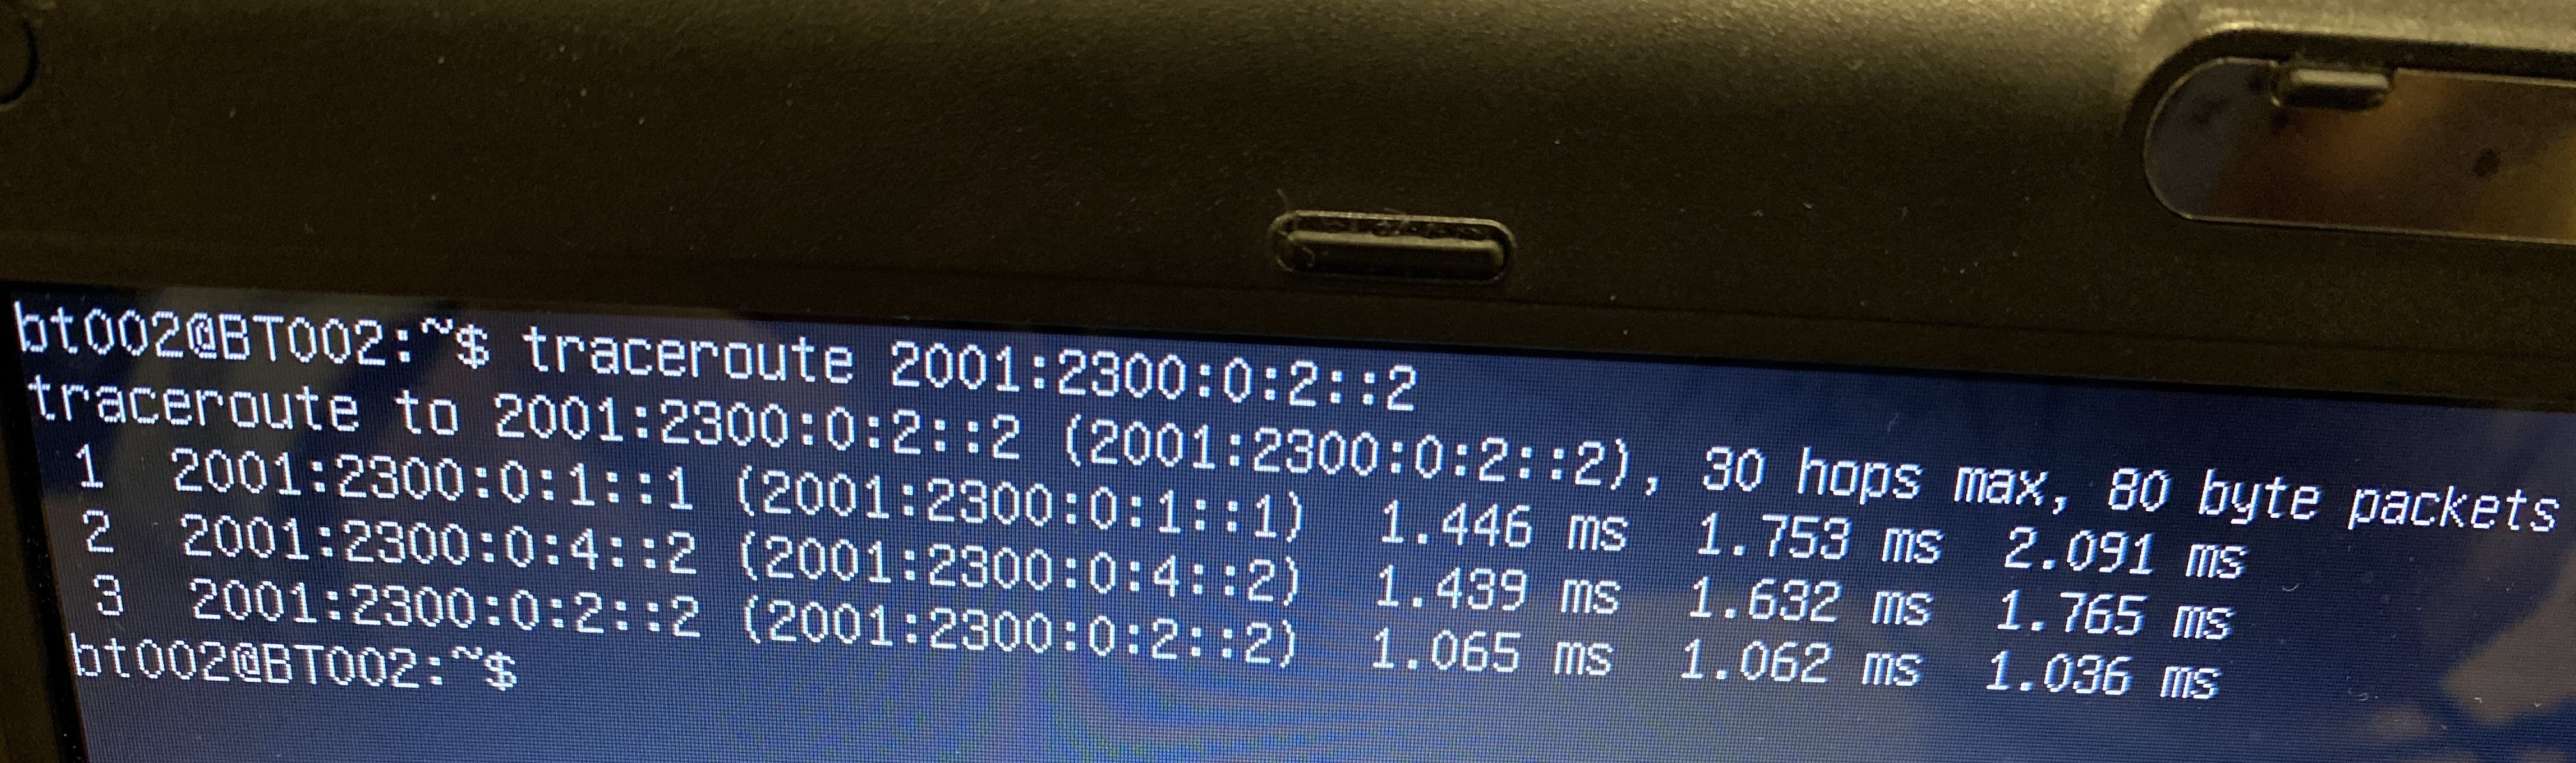
\includegraphics[width=\linewidth]{isis-traceroute-ipv6-2-3}
        \caption{\texttt{traceroute} from Laptop 2 (BT002) to Laptop 3 (BT003)}
    \end{subfigure}
    \caption{Tracing IPv6 Routes between Laptops using \texttt{traceroute}.}
    \label{fig:isis-traceroute-ipv6}
\end{figure}

\clearpage

To further evaluate the correctness of our implementation, we check the path from Laptop 1 to Laptop 2 under the condition that the physical connection between Router 1 and Router 2 is broken. The IS-IS protocol on Router 1 should be able to find route to Router 2 through Router 3.

Figure \ref{fig:isis-traceroute-broken} shows the IPv4 route taken is 
\texttt{Laptop 1 (BT001, IPv6 Address: 23.0.0.2)
-> Router 1 (BT-R001, IPv4 Address: 23.0.0.1) 
-> Router 3 (BT-R003, IPv4 Address: 23.0.0.58) 
-> Router 2 (BT-R002, IPv4 Address: 23.0.0.53)
-> Laptop 2 (BT002, IPv4 Address: 23.0.0.18)}, which is a correct route.


\begin{figure}[ht!]
    \centering
    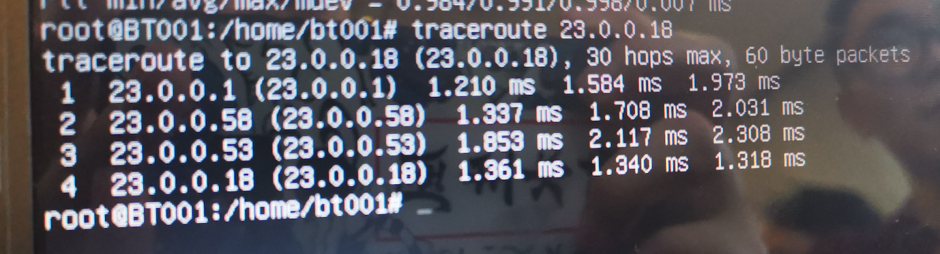
\includegraphics[width=0.8\linewidth]{isis-traceroute-broken-1-2}
    \caption{Tracing IPv4 Routes from Laptop 2 (BT002) to Laptop 3 (BT003) when Physical Connection between Router 1 (BT-R001) and Router 2 (BT-R002) is broken.}
    \label{fig:isis-traceroute-broken}
\end{figure}

Figure \ref{fig:isis-traceroute-broken-ipv6} shows the IPv6 route taken is 
\texttt{Laptop 1 (BT001, IPv6 Address: 2001:2300::2)
-> Router 1 (BT-R001, IPv6 Address: 2001:2300::1) 
-> Router 3 (BT-R003, IPv6 Address: 2001:2300:0:5::2) 
-> Router 2 (BT-R002, IPv6 Address: 2001:2300:0:4::1)
-> Laptop 2 (BT002, IPv6 Address: 2001:2300:0:1::2)}, which is also a correct route.

\begin{figure}[ht!]
    \centering
    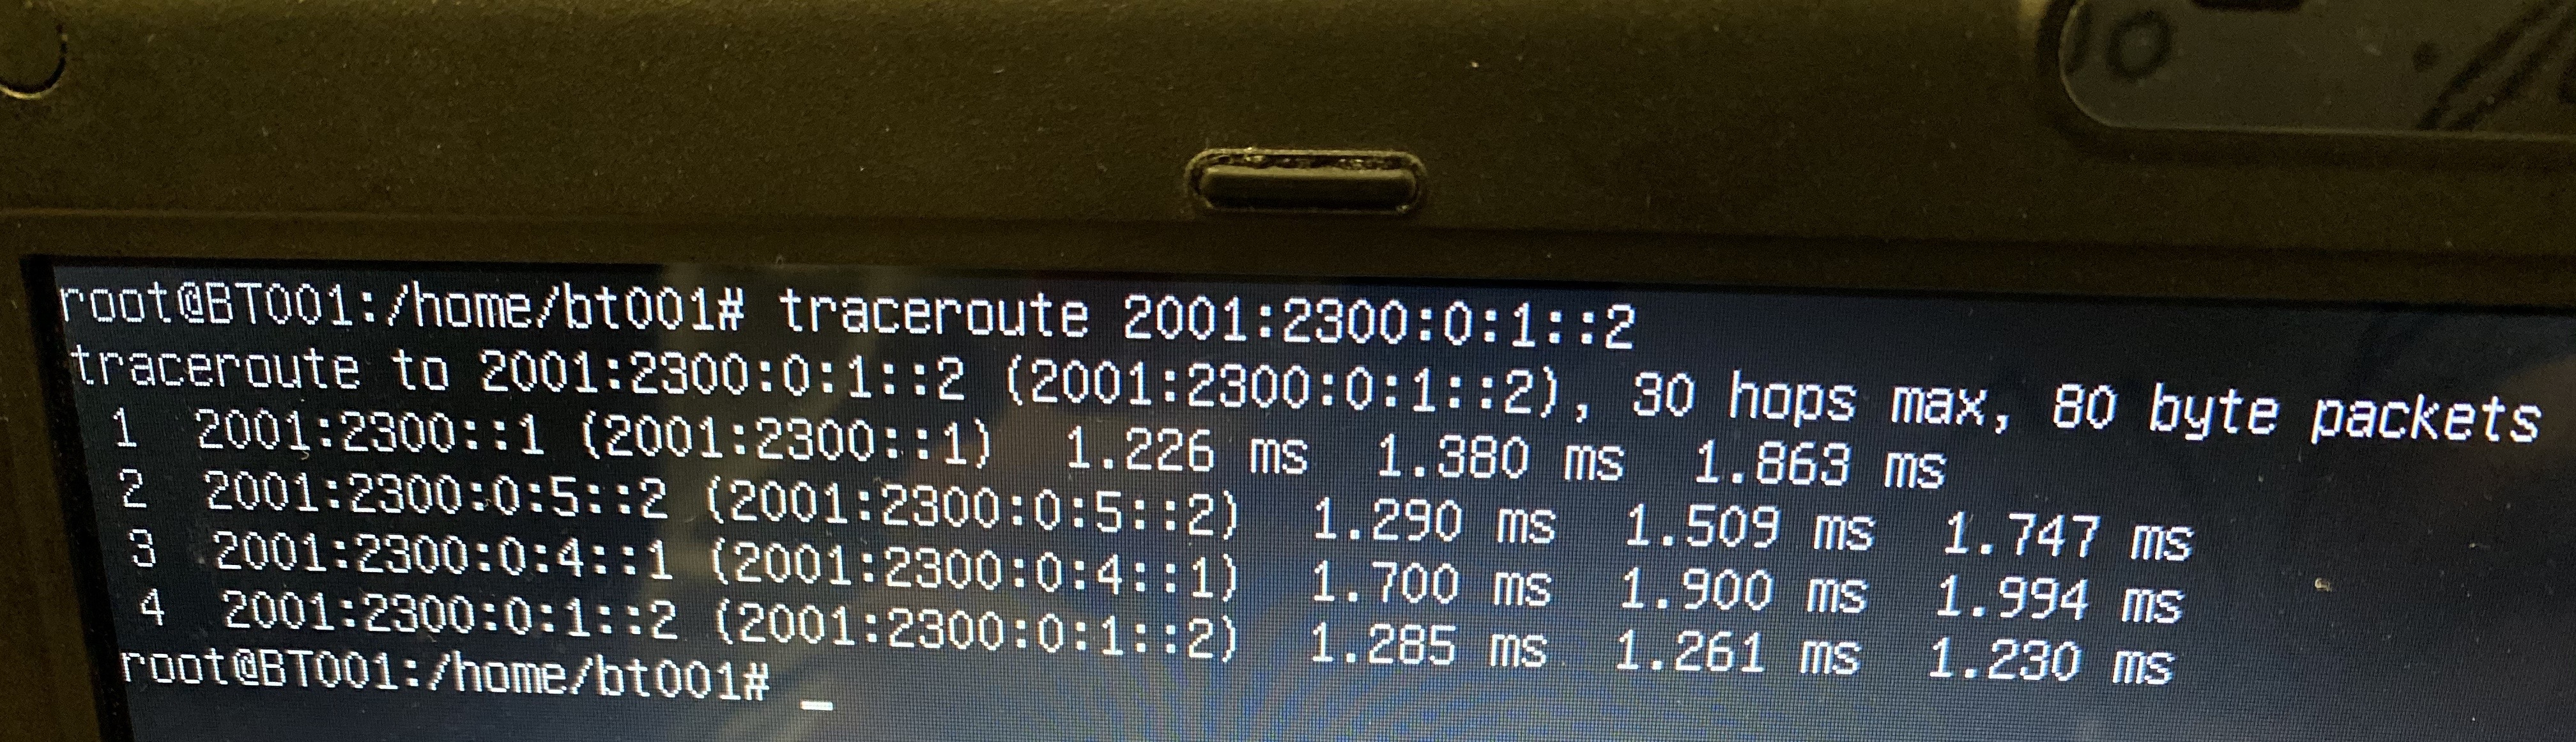
\includegraphics[width=0.8\linewidth]{isis-traceroute-broken-ipv6-1-2}
    \caption{Tracing IPv6 Routes from Laptop 2 (BT002) to Laptop 3 (BT003) when Physical Connection between Router 1 (BT-R001) and Router 2 (BT-R002) is broken.}
    \label{fig:isis-traceroute-broken-ipv6}
\end{figure}

\clearpage

On the router's side, \texttt{show ip route} and \texttt{show ipv6 route} is used to inspect the routes discovered by IS-IS protocol. In Figure \ref{fig:isis-ip-route} and \ref{fig:isis-ipv6-route}, such routes to other subnets inside BT Network on each router are shown.

\begin{figure*}[ht!]
    \centering
    \begin{subfigure}[b]{0.67\textwidth}
        \centering
        \includegraphics[width=\linewidth]{isis-ip-route-1}
        \caption{Router 1 (BT-R001)}
    \end{subfigure}
    \hfill
    \begin{minipage}[b]{0.3\textwidth}
	    \begin{subfigure}[b]{\linewidth}
	        \centering
	        \includegraphics[width=\linewidth]{isis-ip-route-2}
	        \caption{Router 2 (BT-R002)}
	    \end{subfigure}
	    \\
	    \begin{subfigure}[b]{\linewidth}
	        \centering
	        \includegraphics[width=\linewidth]{isis-ip-route-3}
	        \caption{Router 3 (BT-R003)}
	    \end{subfigure}
	\end{minipage}
    \caption{IPv4 Routes to Other Subnets on All $3$ Routers Respectively using \texttt{show ip route}.}
    \label{fig:isis-ip-route}
\end{figure*}


\begin{figure*}[ht!]
    \centering
    \begin{subfigure}[b]{0.67\textwidth}
        \centering
        \includegraphics[width=\linewidth]{isis-ipv6-route-1}
        \caption{Router 1 (BT-R001)}
    \end{subfigure}
    \hfill
    \begin{minipage}[b]{0.3\textwidth}
	    \begin{subfigure}[b]{\linewidth}
	        \centering
	        \includegraphics[width=\linewidth]{isis-ipv6-route-2}
	        \caption{Router 2 (BT-R002)}
	    \end{subfigure}
	    \\
	    \begin{subfigure}[b]{\linewidth}
	        \centering
	        \includegraphics[width=\linewidth]{isis-ipv6-route-3}
	        \caption{Router 3 (BT-R003)}
	    \end{subfigure}
	\end{minipage}
    \caption{IPv6 Routes to Other Subnets on All $3$ Routers Respectively using \texttt{show ipv6 route}.}
    \label{fig:isis-ipv6-route}
\end{figure*}

\clearpage

Noticably, when the physical connection between Router 1 and Router 2 is broken, the route from Router 1 to Router 2 goes through Router 3 instead, as evident in Figure \ref{fig:isis-ip-route-broken}.

\begin{figure}[ht!]
    \centering    
    \begin{subfigure}[b]{\textwidth}
        \centering
        \includegraphics[width=\linewidth]{isis-ip-route-broken-1}
        \caption{IPv4 Routes to Other Subnets on Router 1 using \texttt{show ip route}.}
    \end{subfigure}
    ~
    \begin{subfigure}[b]{\textwidth}
        \centering
        \includegraphics[width=\linewidth]{isis-ipv6-route-broken-1}
        \caption{IPv6 Routes to Other Subnets on Router 1 using \texttt{show ip route}.}
    \end{subfigure}
    \caption{IP Routes to Other Subnets on Router 1 when Physical Connection between Router 1 (BT-R001) and Router 2 (BT-R002) is broken.}
    \label{fig:isis-ip-route-broken}
\end{figure}

\subsection{Commentary}

\subsubsection{Problem: IS-IS Not Set Up for Laptop-Router Interface}
When initially setting up IS-IS on the interfaces, only the interfaces between routers have been turned on. This leads to laptop's failure to reach a router not directly connected.
To solve this problem, IS-IS is set up on the interface between a laptop and a router.

\subsubsection{Alternative Solution to Passive Interfaces}
While turning interfaces connected to outside network into passive interfaces does enable other routers in the network to connect to outside networks through those interfaces, it demands extra computing resource for computing routes to external subnets. 

\textbf{Alternatively, one can disable IS-IS on such interfaces and replace the external next-hop for each out-going route in BGP with the internal router to which the next-hop is directly connected to. That prevents Router-Neighbour subnet from participating in IS-IS routing and eliminates the extra computing consumption while preserving the connectivity between internal routers and outside networks.}


\clearpage




\newpage
\section{Inter-domain Routing Protocol: BGP}
\label{sec:bgp}

\subsection{Design}
For inter-domain routing, Border Gateway Protocol (BGP)\citep{rfc4271} is applied in BT Network since it's the one and only External Gateway Protocol (EGP) in today's global Internet. BGP provides scaliability to large networks, clear definations of administrative boudnary as well as flexiable policy control, which allow business relaitonships with neighbouring ISPs to be expressed in terms of routing policies.

Figure \ref{fig:bgp} shows the design of BGP protocol in our network. The AS Number (ASN) of BT Network is 2030 while ASN of Central, Virgin, DT are 42, 5060, 3040 respectively. 

\begin{figure}[ht!]
    \centering
    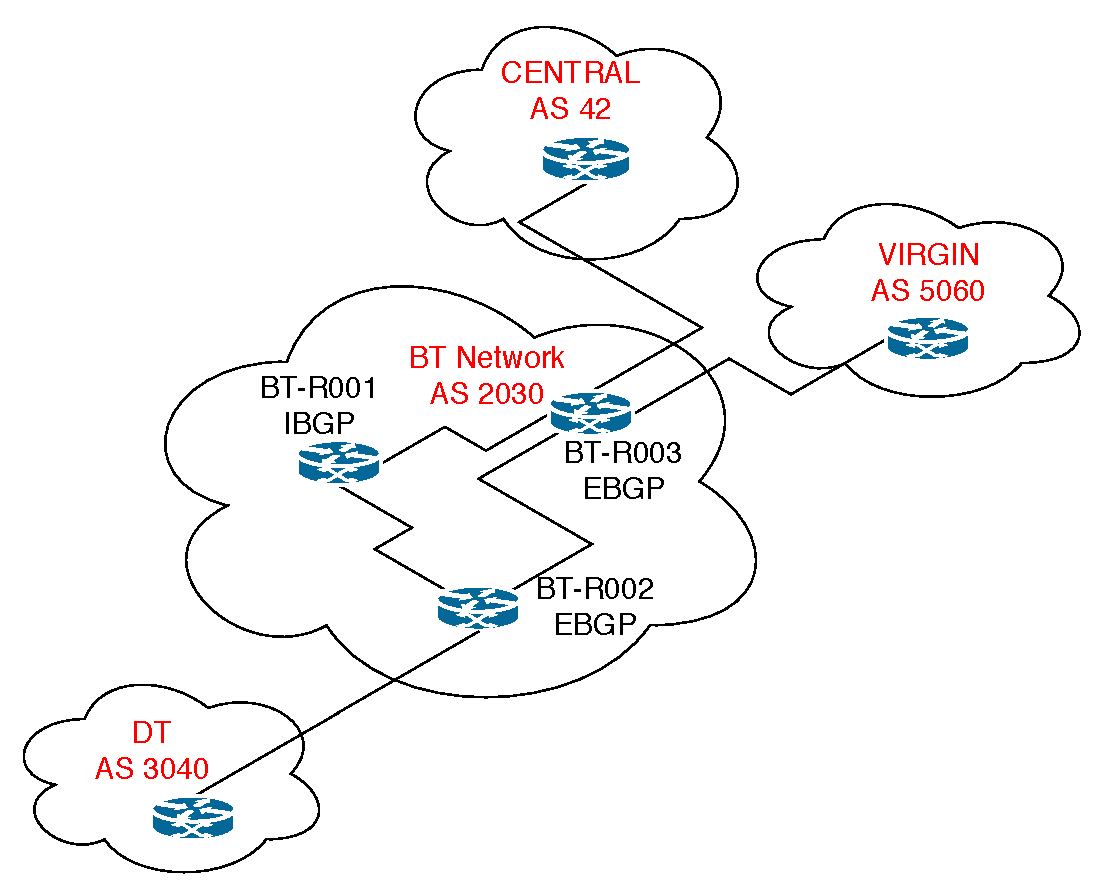
\includegraphics[width=\linewidth]{bgp}
    \caption{Design of BGP Protocol in BT Network.}
    \label{fig:bgp}
\end{figure}

Router 2 (BT-R002) and Router 3 (BT-R003) act as External BGP routers since they are directly connected to neighbouring ISPs. They receive routes announced by neighbouring ISPs' routers and announce routes originated from BT Network.
Router 1 (BT-R001) acts as an Internal BGP (IBGP) router only since it is not directly connected to any neighbouring ISP and only forwards and receives routes announced by EGBP routers.




\subsection{Routing Policies}

To enact business relationships with neighbouring ISPs, proper routing polices should be implemented for each different relationship in BGP protocol. 
Specifically, for customer ISPs, all routes announced by such ISP should be accepted and all routes received should be annouced to it as well. This allows customers to connect to BT Network as well as connect to other networks through BT Network.

For non-customer neighbouring ISPs (peers and providers), all routes announced by such ISP should be accepted in order for BT Network to connect to it. Meanwhile, only routes originated from either BT Network or BT's customers are announced to such ISP.

\subsection{Implementation}

On Router 1 (BT-R001, IPv4 Loopback Address: \texttt{23.0.255.1}, IPv6 Loopback Address: \texttt{2001:2300:FFFF:1::}), both Router 2 (BT-R002, IPv4 Loopback Address: \texttt{23.0.255.2}, IPv6 Loopback Address: \texttt{2001:2300:FFFF:2::}) and Router 3 (BT-R003, IPv4 Loopback Address: \texttt{23.0.255.3}, IPv6 Loopback Address: \texttt{2001:2300:FFFF:3::}) are taken as neighbouring routers in the same AS.
In addition, the source of BGP messages are set to be the loopback address of Router 1 to prevent physical disconnection to the $2$ routers.
Router 1 announces the subnet \texttt{BT-R001 - BT001} (IPv4: \texttt{23.0.0.0/28}, IPv6: \texttt{2001:2300:0:0::/64}) to other routers.

\begin{lstlisting}
router bgp 2030
network 23.0.0.0 mask 255.255.255.240
neighbor 23.0.255.2 remote-as 2030
neighbor 23.0.255.2 update-source Loopback0
neighbor 23.0.255.3 remote-as 2030
neighbor 23.0.255.3 update-source Loopback0
neighbor 2001:2300:FFFF:2:: remote-as 2030
neighbor 2001:2300:FFFF:2:: update-source Loopback0
neighbor 2001:2300:FFFF:3:: remote-as 2030
neighbor 2001:2300:FFFF:3:: update-source Loopback0

address-family ipv6
network 2001:2300::/64
neighbor 2001:2300:FFFF:2:: activate
neighbor 2001:2300:FFFF:3:: activate
\end{lstlisting}

On Router 2 (BT-R002), both Router 1 and Router 3 are taken as neighbouring routers in the same AS while the router from DT is taken as router from AS 3040.
Router 2 announces the subnet \texttt{BT-R002 - BT002} (IPv4: \texttt{23.0.0.16/28}, IPv6: \texttt{2001:2300:0:1::/64}) to other routers.
Since Router 2 is direclty connected to customer DT Network, it applies no filter on inbound and outbound routes.

\begin{lstlisting}
router bgp 2030
network 23.0.0.16 mask 255.255.255.240
neighbor 23.0.0.62 remote-as 3040
neighbor 23.0.255.1 remote-as 2030
neighbor 23.0.255.1 update-source Loopback0
neighbor 23.0.255.3 remote-as 2030
neighbor 23.0.255.3 update-source Loopback0
neighbor 2001:2300:0:6::2 remote-as 3040
neighbor 2001:2300:FFFF:1:: remote-as 2030
neighbor 2001:2300:FFFF:1:: update-source Loopback0
neighbor 2001:2300:FFFF:3:: remote-as 2030
neighbor 2001:2300:FFFF:3:: update-source Loopback0

address-family ipv6
network 2001:2300:0:1::/64
neighbor 2001:2300:0:6::2 activate
neighbor 2001:2300:FFFF:1:: activate
neighbor 2001:2300:FFFF:3:: activate
\end{lstlisting}

On Router 3 (BT-R003), both Router 1 and Router 2 are taken as neighbouring routers in the same AS while the routers from Central and Virgin are taken as router from AS 42 and AS 5060 respectively.
Router 3 announces the subnet \texttt{BT-R003 - BT003} (IPv4: \texttt{23.0.0.32/28}, IPv6: \texttt{2001:2300:0:2::/64}) to other routers.

\begin{lstlisting}
router bgp 2030
network 23.0.0.32 mask 255.255.255.240
neighbor 23.0.255.1 remote-as 2030
neighbor 23.0.255.1 update-source Loopback0
neighbor 23.0.255.2 remote-as 2030
neighbor 23.0.255.2 update-source Loopback0
neighbor 2001:2300:FFFF:1:: remote-as 2030
neighbor 2001:2300:FFFF:1:: update-source Loopback0
neighbor 2001:2300:FFFF:2:: remote-as 2030
neighbor 2001:2300:FFFF:2:: update-source Loopback0
neighbor 2001:5600:0:6::1 remote-as 5060
neighbor 56.0.0.61 remote-as 5060
neighbor 100.100.2.1 remote-as 42

address-family ipv6
network 2001:2300:0:2::/64
aggregate-address 2001:2300::/32 summary-only
neighbor 2001:2300:FFFF:1:: activate
neighbor 2001:2300:FFFF:2:: activate
\end{lstlisting}


Since Router 3 is direclty connected to non-customer ISPs, it applies a filter on outbound routes, which denies all routes that pass through either Central Network (ASN: $42$) or Virgin Network (ASN: $5060$).

\begin{lstlisting}
ip as-path access-list 1 deny _42_
ip as-path access-list 1 deny _5060_
ip as-path access-list 1 permit .*
router bgp 2030
neighbor 56.0.0.61 filter-list 1 out
neighbor 100.100.2.1 filter-list 1 out
\end{lstlisting}

Address aggregation for \texttt{23.0.0.0/8} and \texttt{2001:2300::/32} is set up on all 3 routers, which aggregates routes destined for all addresses inside BT Network range into a single route.

\begin{lstlisting}
aggregate-address 23.0.0.0 255.0.0.0 summary-only
address-family ipv6
aggregate-address 2001:2300::/32 summary-only
\end{lstlisting}


\subsection{Evaluation}

\subsubsection{BGP Routes}

Routes collected through BGP protocol on all $3$ routers are shown in Figure \ref{fig:bgp-route} and \ref{fig:bgp-route-ipv6} using commands \texttt{show bgp} and \texttt{show bgp ipv6}. 
Routes to DT Network (IPv4: \texttt{34.0.0.0/8}, IPv6: \texttt{2001:3400::/32}), Virgin Network (IPv4: \texttt{56.0.0.0/8}, IPv6: \texttt{2001:5600::/32}), Central Network (IPv4: \texttt{10.2.2.0/24}) and other networks can be observed in the figure.

\begin{figure*}[ht!]
    \centering
    \begin{subfigure}[b]{0.67\textwidth}
        \centering
        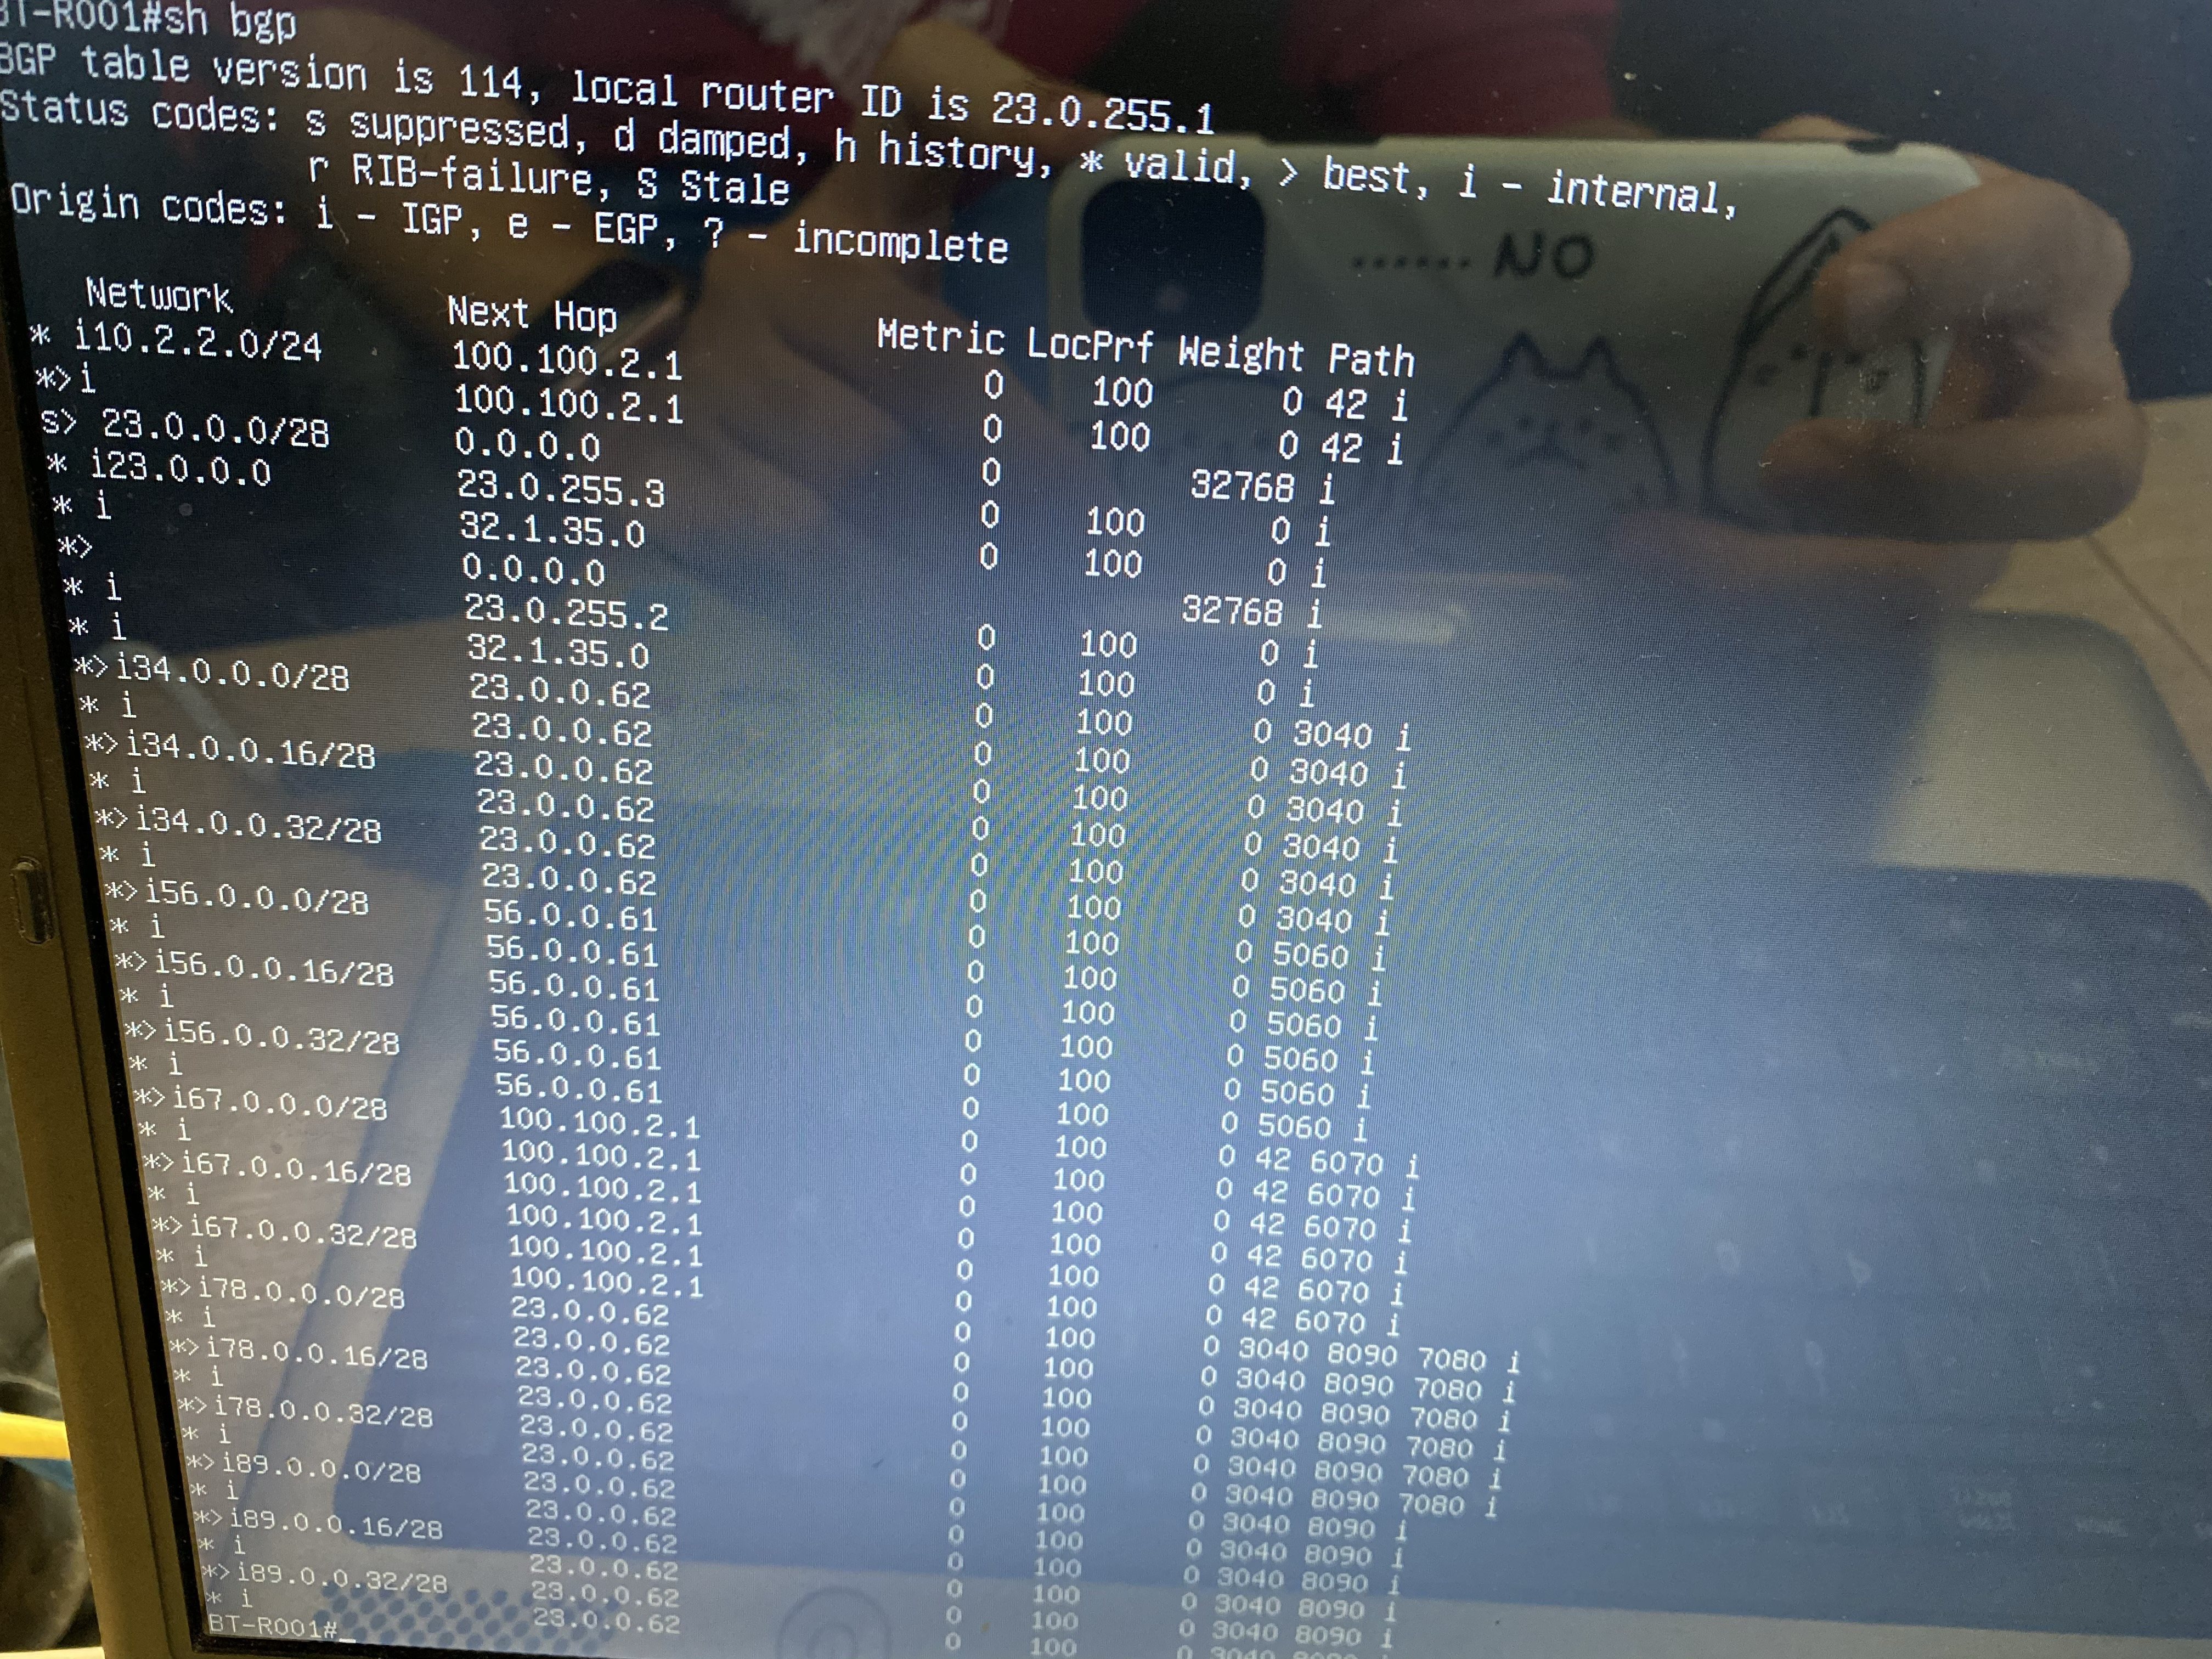
\includegraphics[width=\linewidth]{bgp-route-1}
        \caption{Router 1 (BT-R001)}
    \end{subfigure}
    \hfill
    \begin{minipage}[b]{0.3\textwidth}
	    \begin{subfigure}[b]{\linewidth}
	        \centering
	        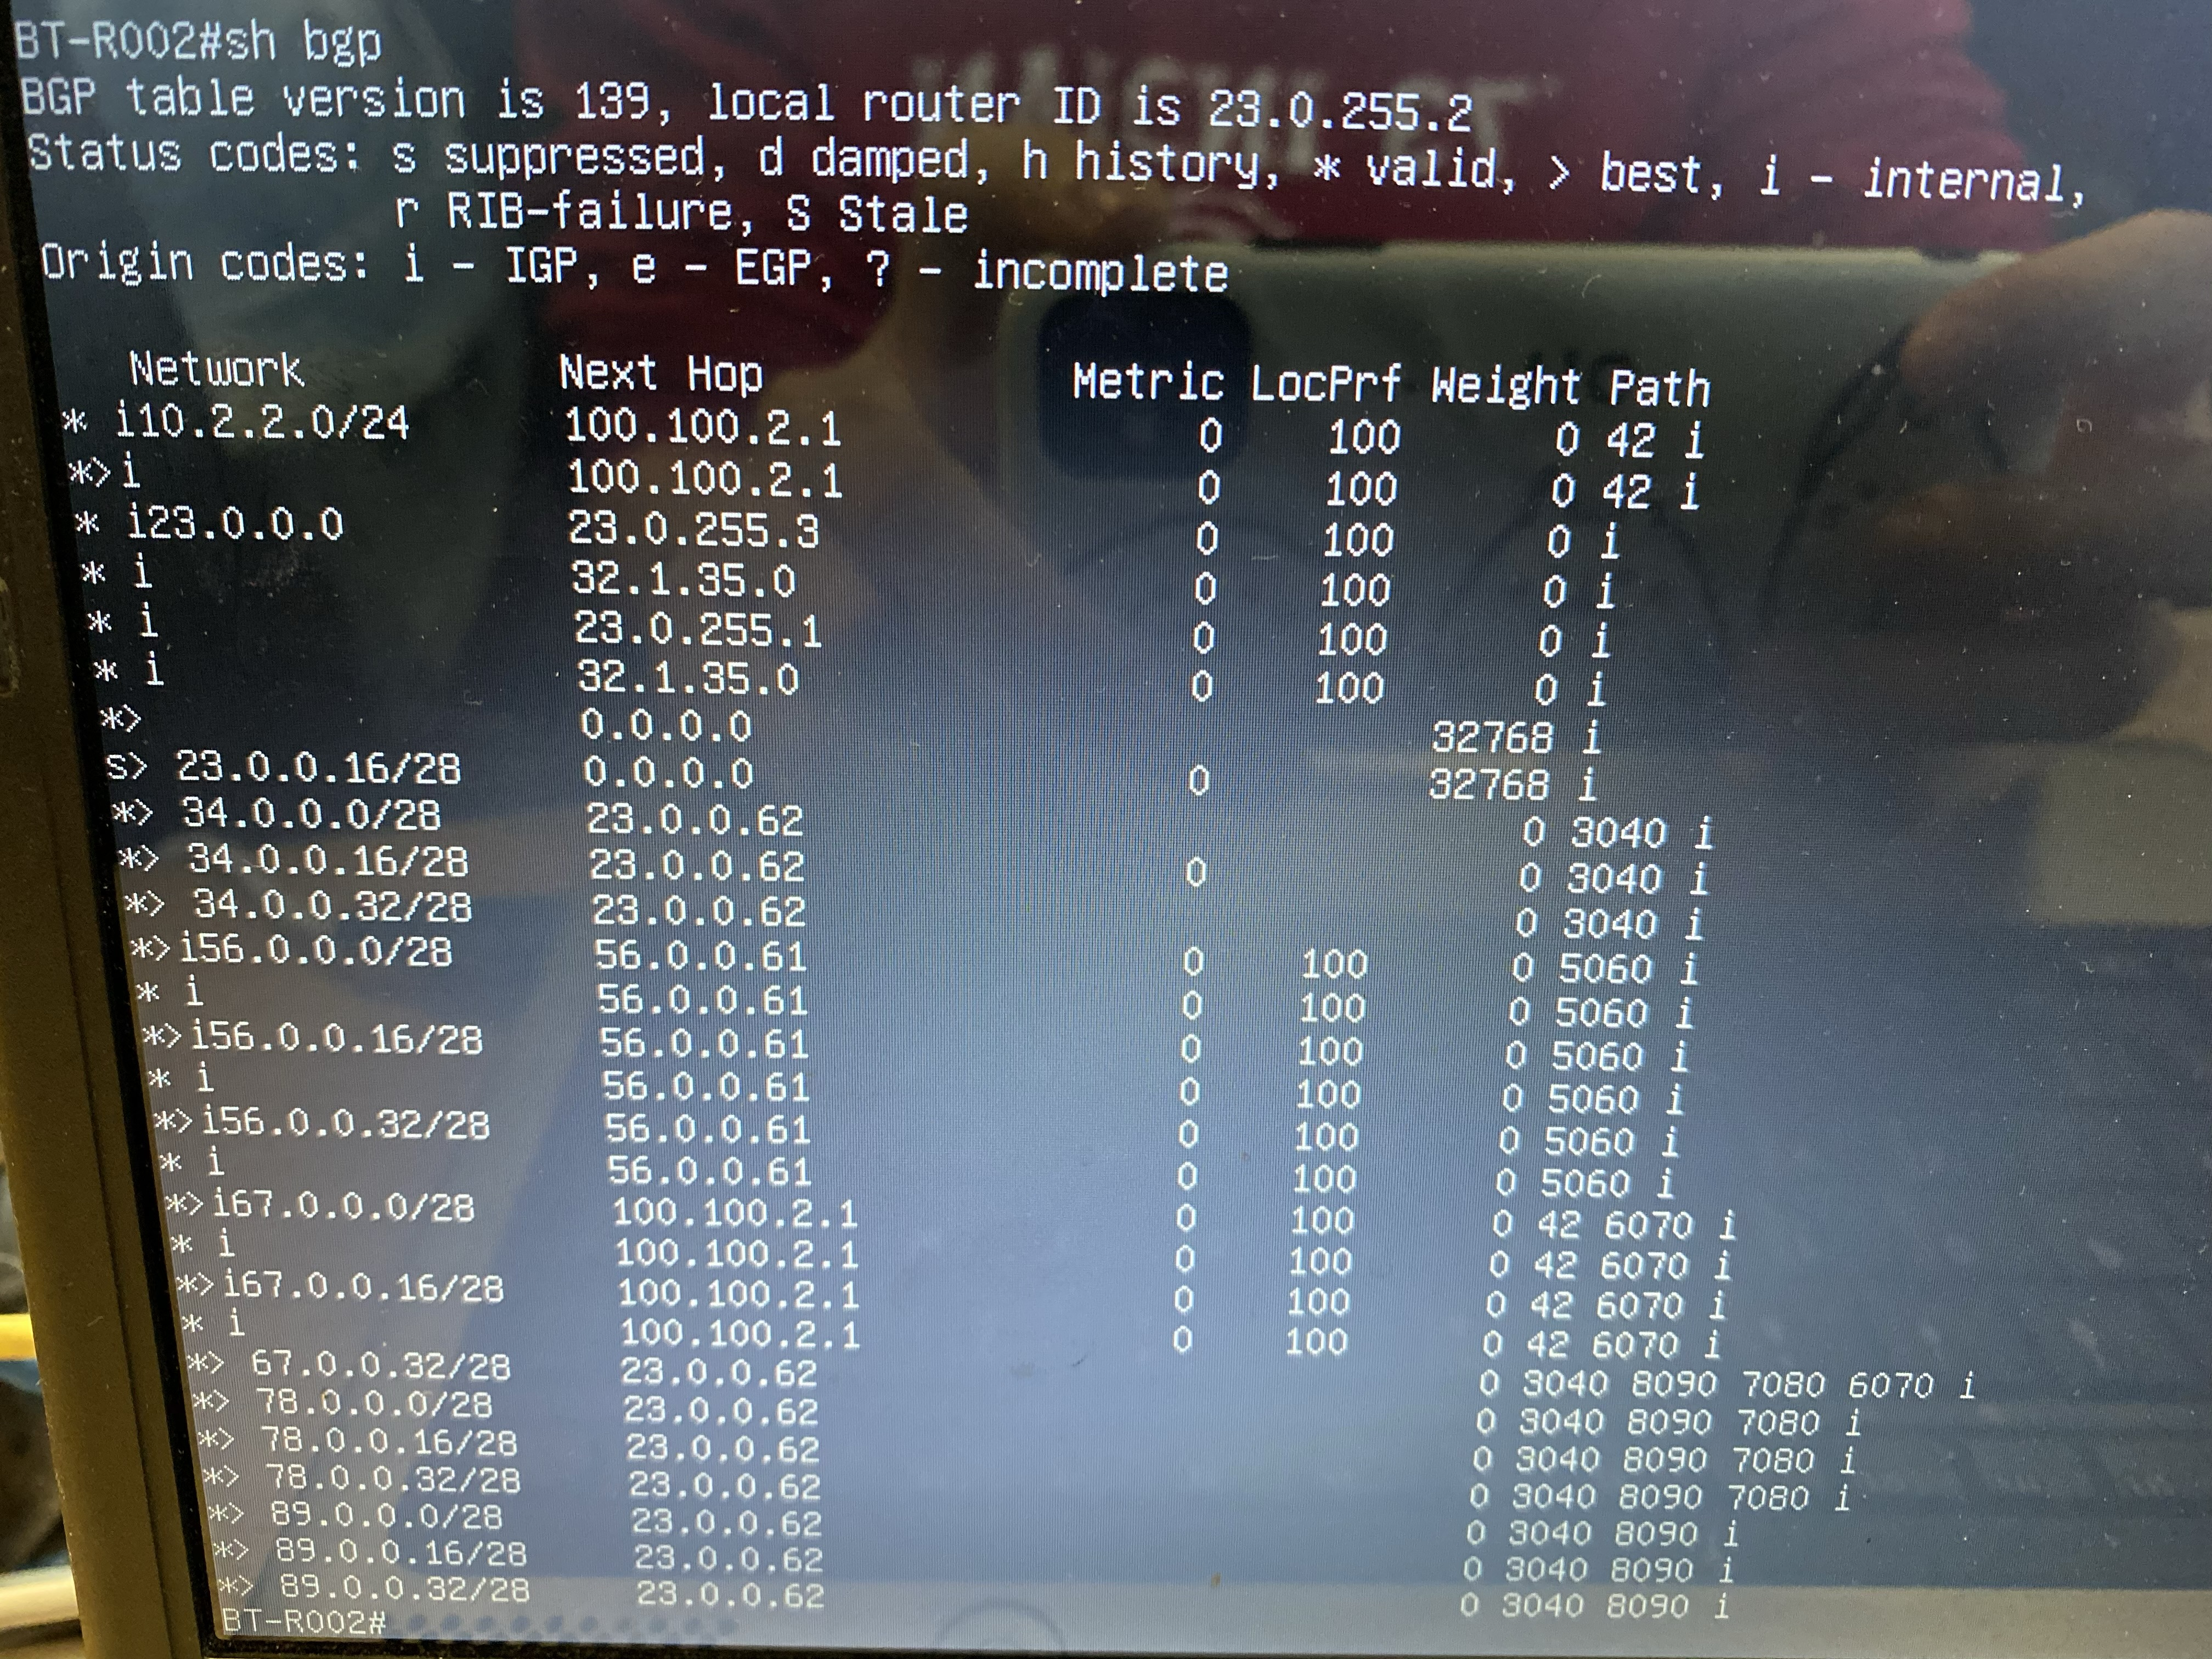
\includegraphics[width=\linewidth]{bgp-route-2}
	        \caption{Router 2 (BT-R002)}
	    \end{subfigure}
	    \\
	    \begin{subfigure}[b]{\linewidth}
	        \centering
	        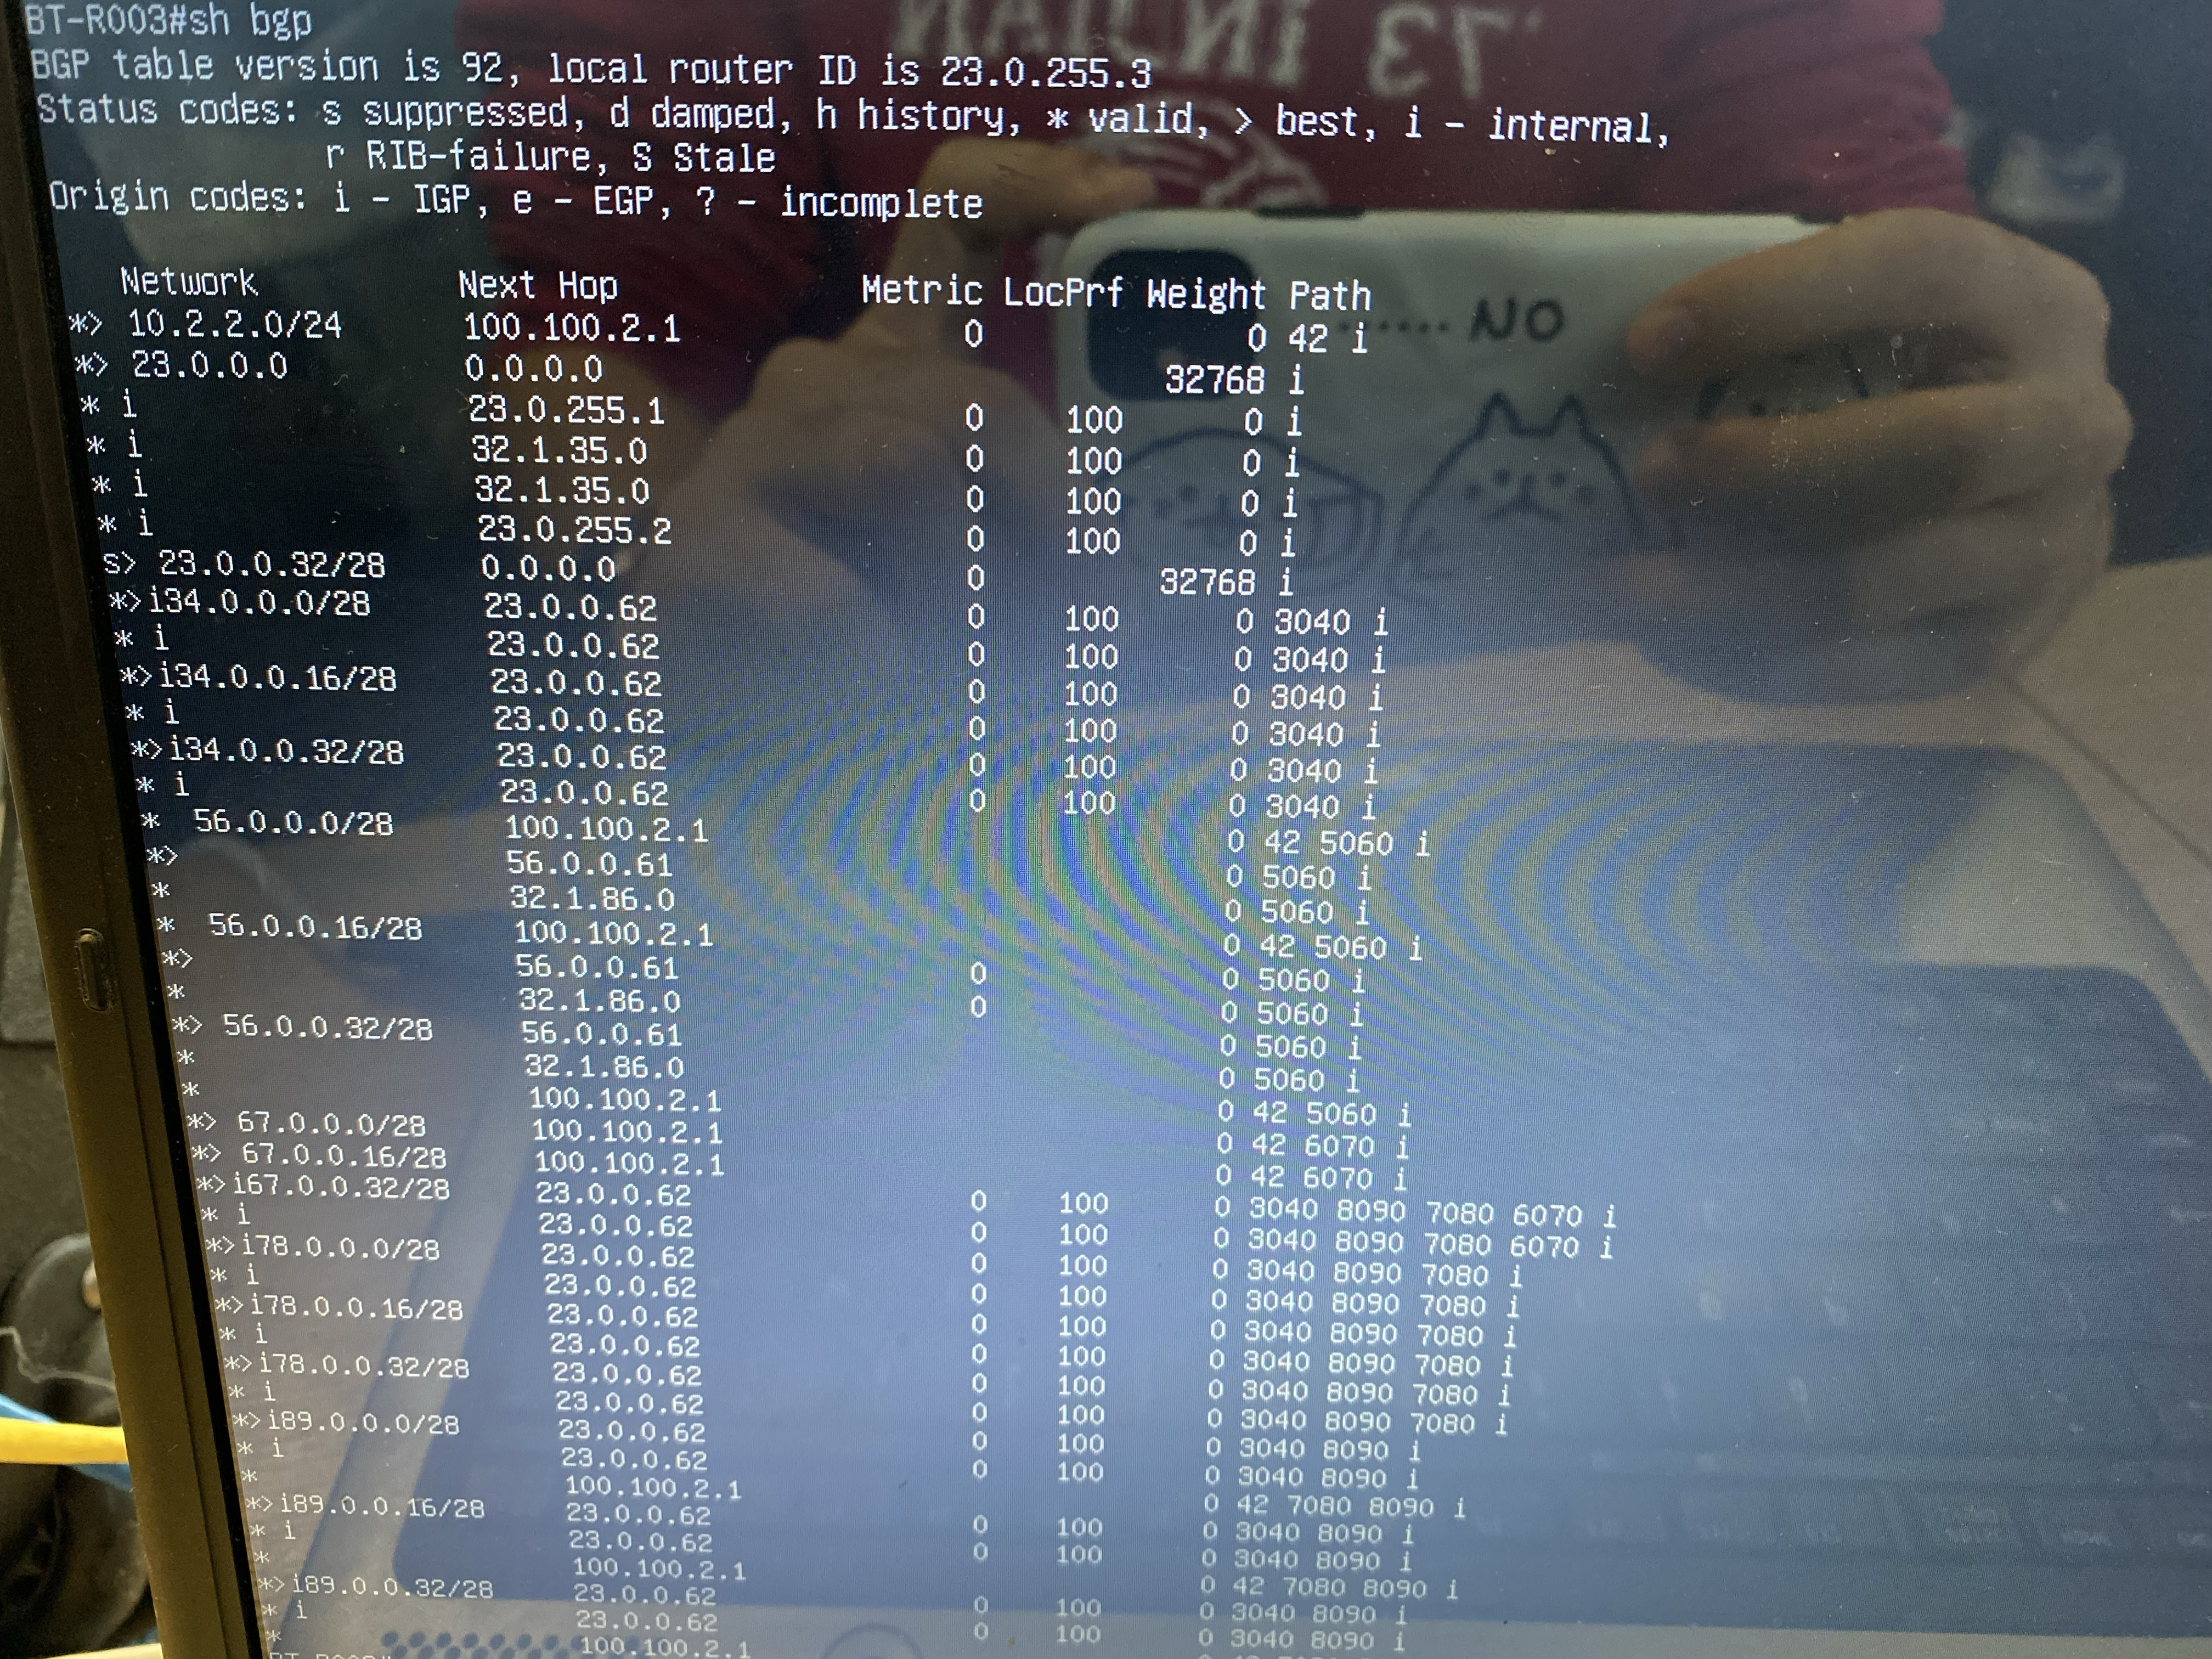
\includegraphics[width=\linewidth]{bgp-route-3}
	        \caption{Router 3 (BT-R003)}
	    \end{subfigure}
	\end{minipage}
    \caption{IPv4 Routes Collected through BGP Protocols on All $3$ Routers using \texttt{show bgp}.}
    \label{fig:bgp-route}
\end{figure*}



\clearpage


\subsubsection{Connectivity to Provider Central Network}

The connectivity to provider Central Network using BGP protocol is tested and evaluated by tracing routes to IP addresses \texttt{10.2.2.1} on Laptop 1 (BT001). As shown in Figure \ref{fig:bgp-central}, connection to Central Network is successfully established through BGP routes.

\begin{figure*}[ht!]
    \centering
    \begin{subfigure}[b]{\textwidth}
        \centering
        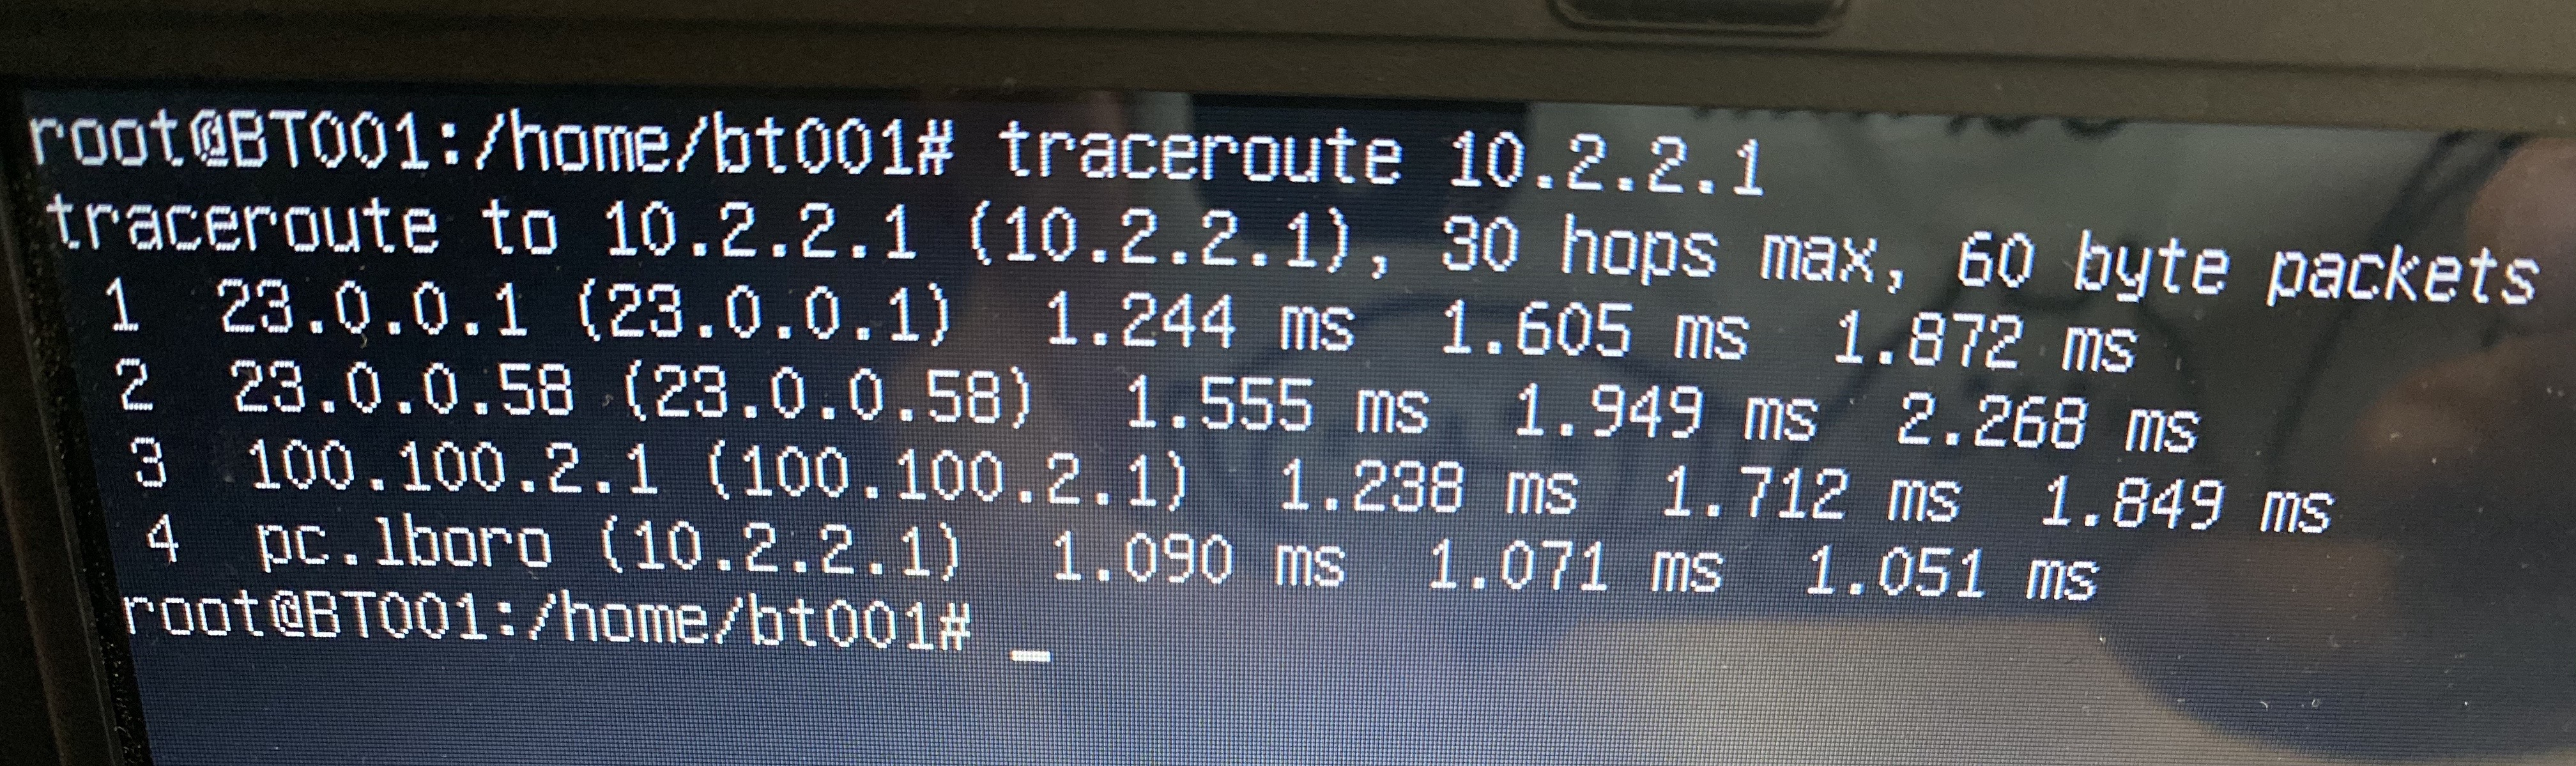
\includegraphics[width=\linewidth]{bgp-central-1}
        \caption{\texttt{10.2.2.1}}
    \end{subfigure}
    ~
    % \begin{subfigure}[b]{0.67\textwidth}
    %     \centering
    %     \includegraphics[width=\linewidth]{bgp-central-2}
    %     \caption{\texttt{10.2.2.253}}
    % \end{subfigure}
    \caption{Tracing IPv4 Routes to Central Network on Laptop 1 (BT001) using \texttt{traceroute}.}
    \label{fig:bgp-central}
\end{figure*}


\clearpage


\subsubsection{Connectivity to Customer DT Network}
The connectivity to customer DT Network using BGP protocol is tested and evaluated by tracing routes to IP addresses \texttt{34.0.0.2}, \texttt{34.0.0.18} and \texttt{34.0.0.34} on Laptop 1 (BT001). As shown in Figure \ref{fig:bgp-dt}, connection to DT Network is successfully established through BGP routes.

\begin{figure*}[ht!]
    \centering
    \begin{subfigure}[b]{\textwidth}
        \centering
        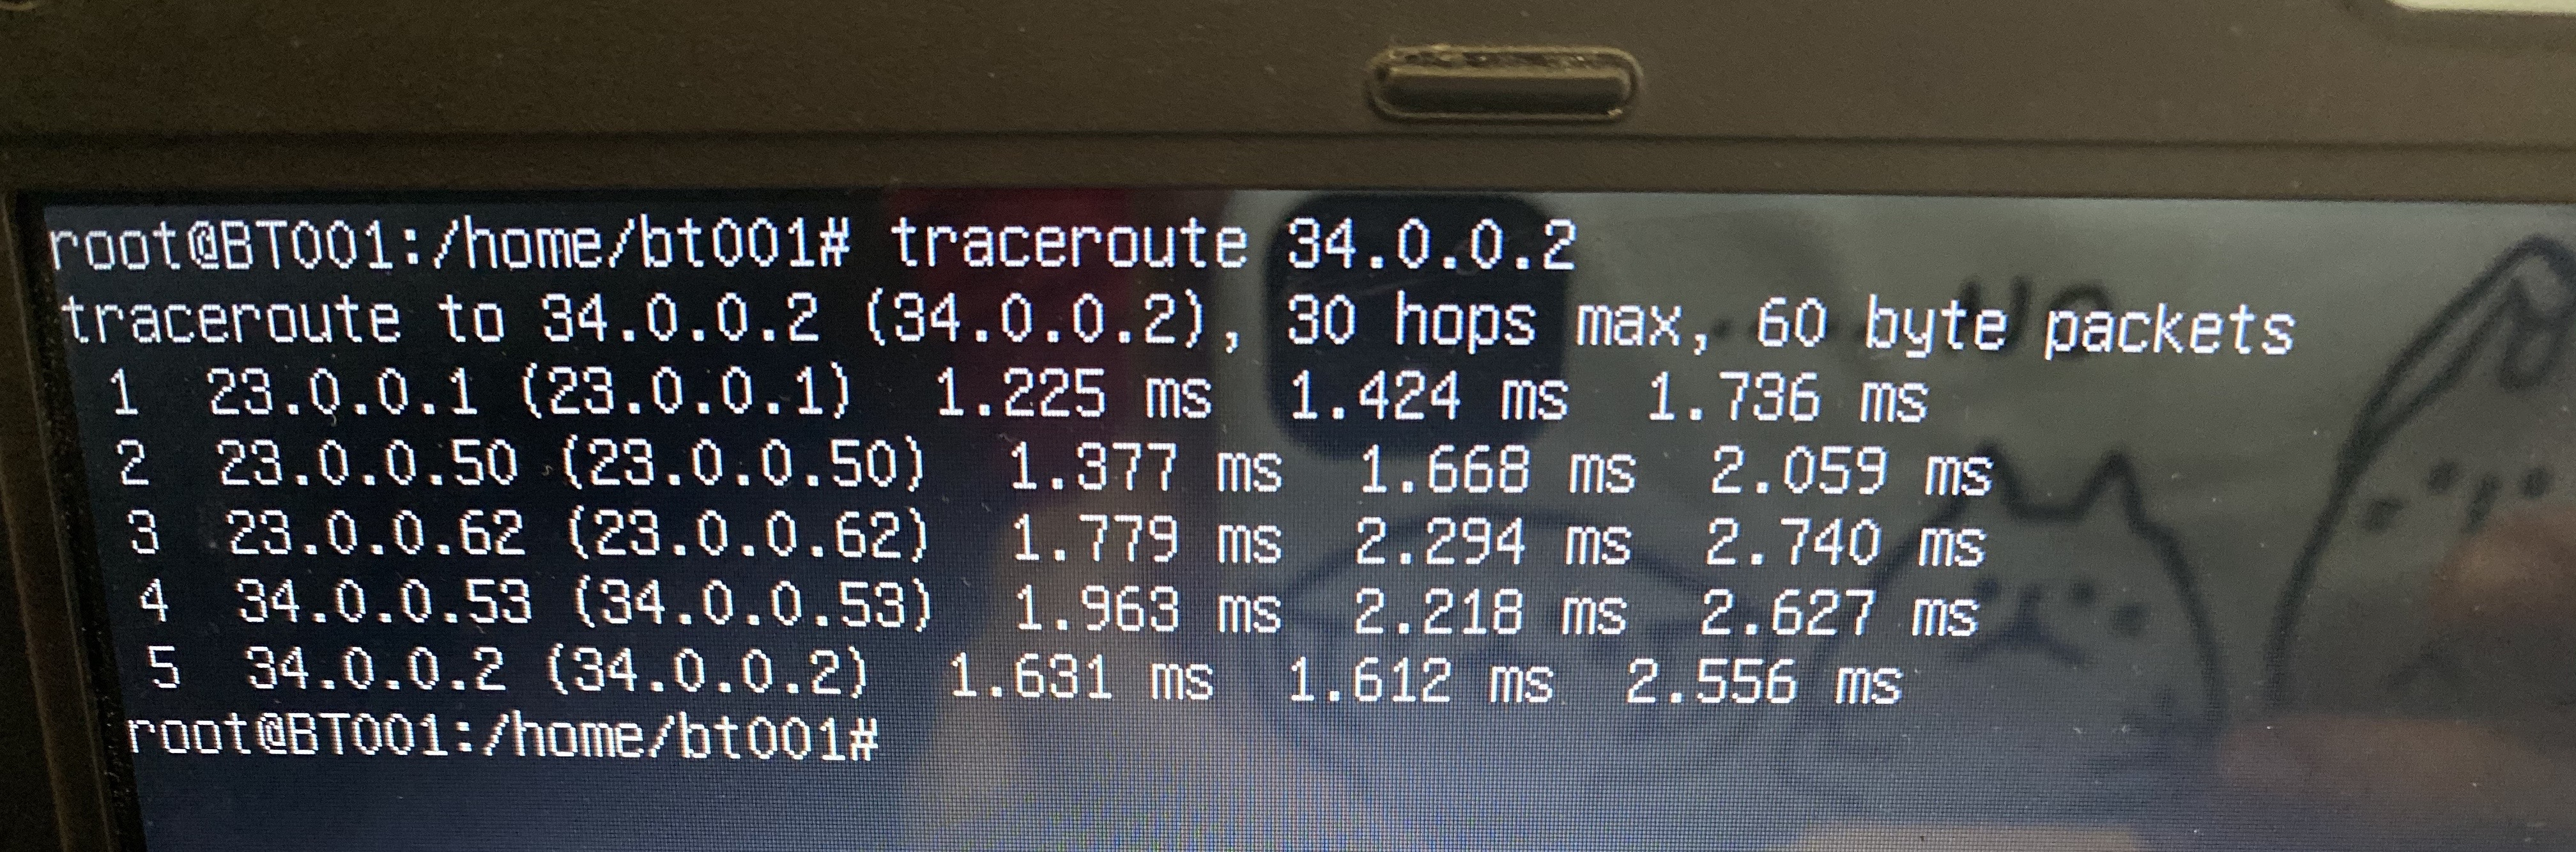
\includegraphics[width=\linewidth]{bgp-dt-1}
        \caption{\texttt{34.0.0.2}}
    \end{subfigure}
    ~
    \begin{subfigure}[b]{\textwidth}
        \centering
        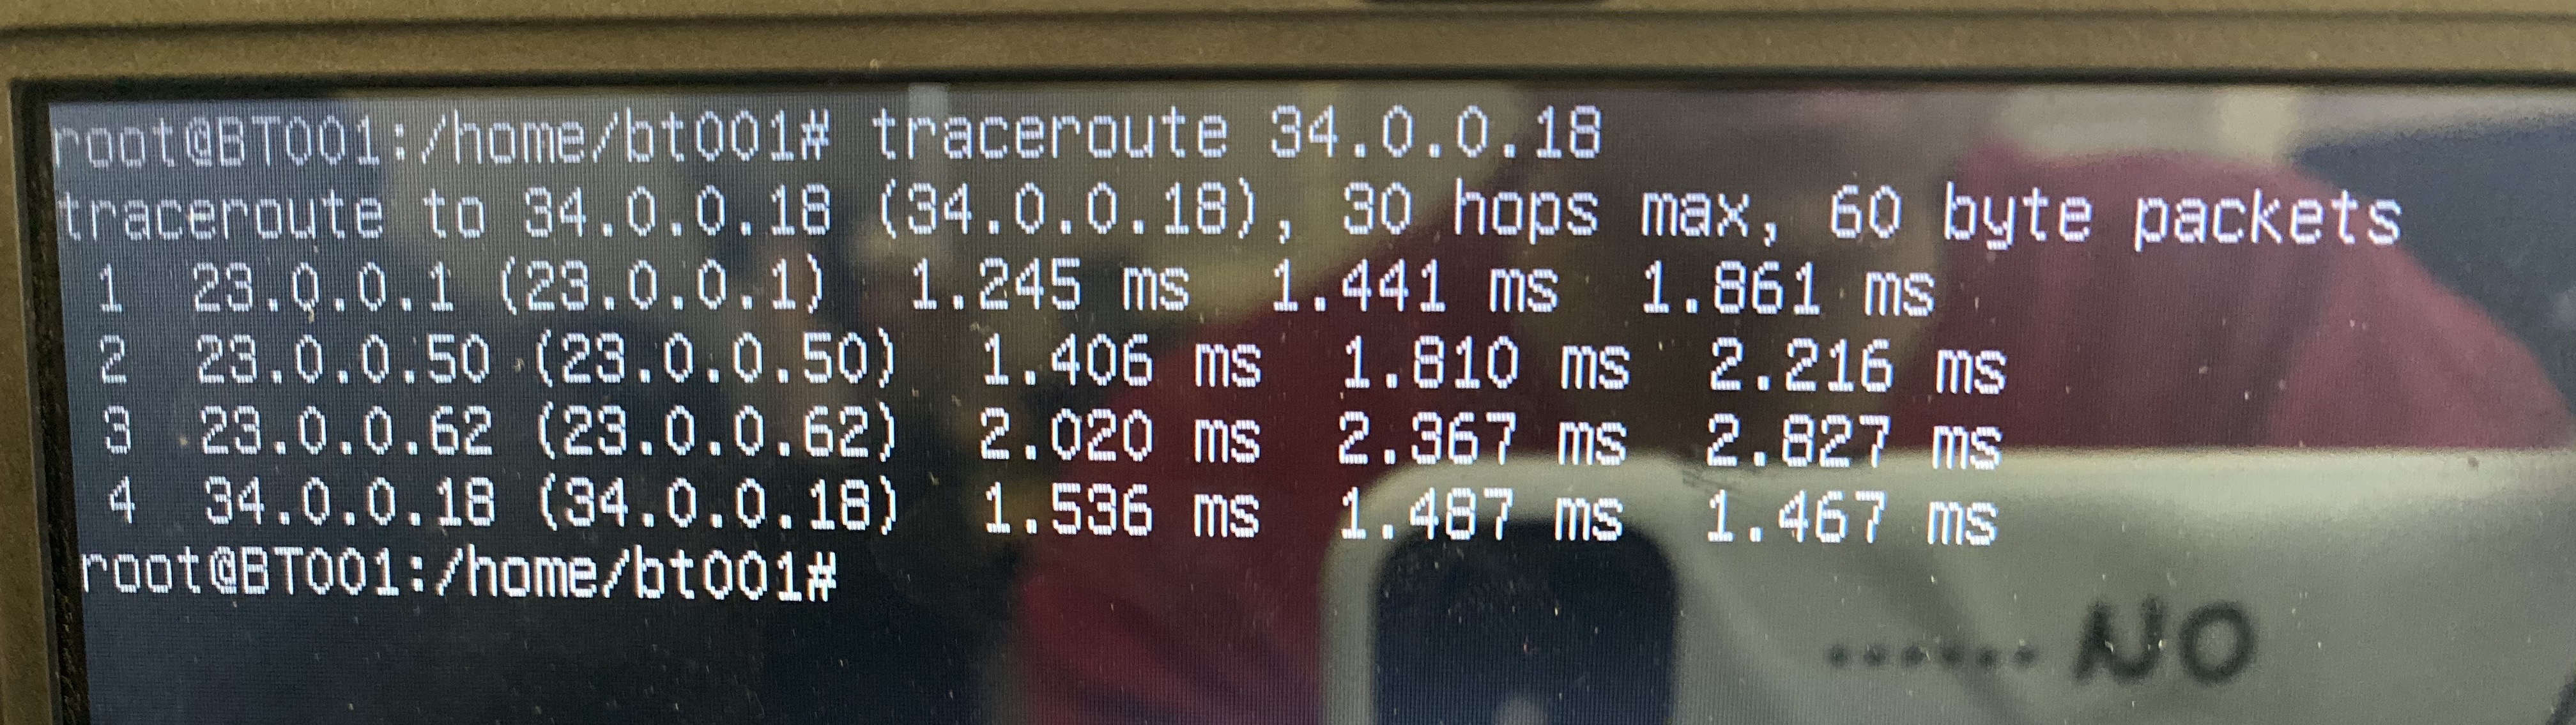
\includegraphics[width=\linewidth]{bgp-dt-2}
        \caption{\texttt{34.0.0.18}}
    \end{subfigure}
    ~
    \begin{subfigure}[b]{\textwidth}
        \centering
        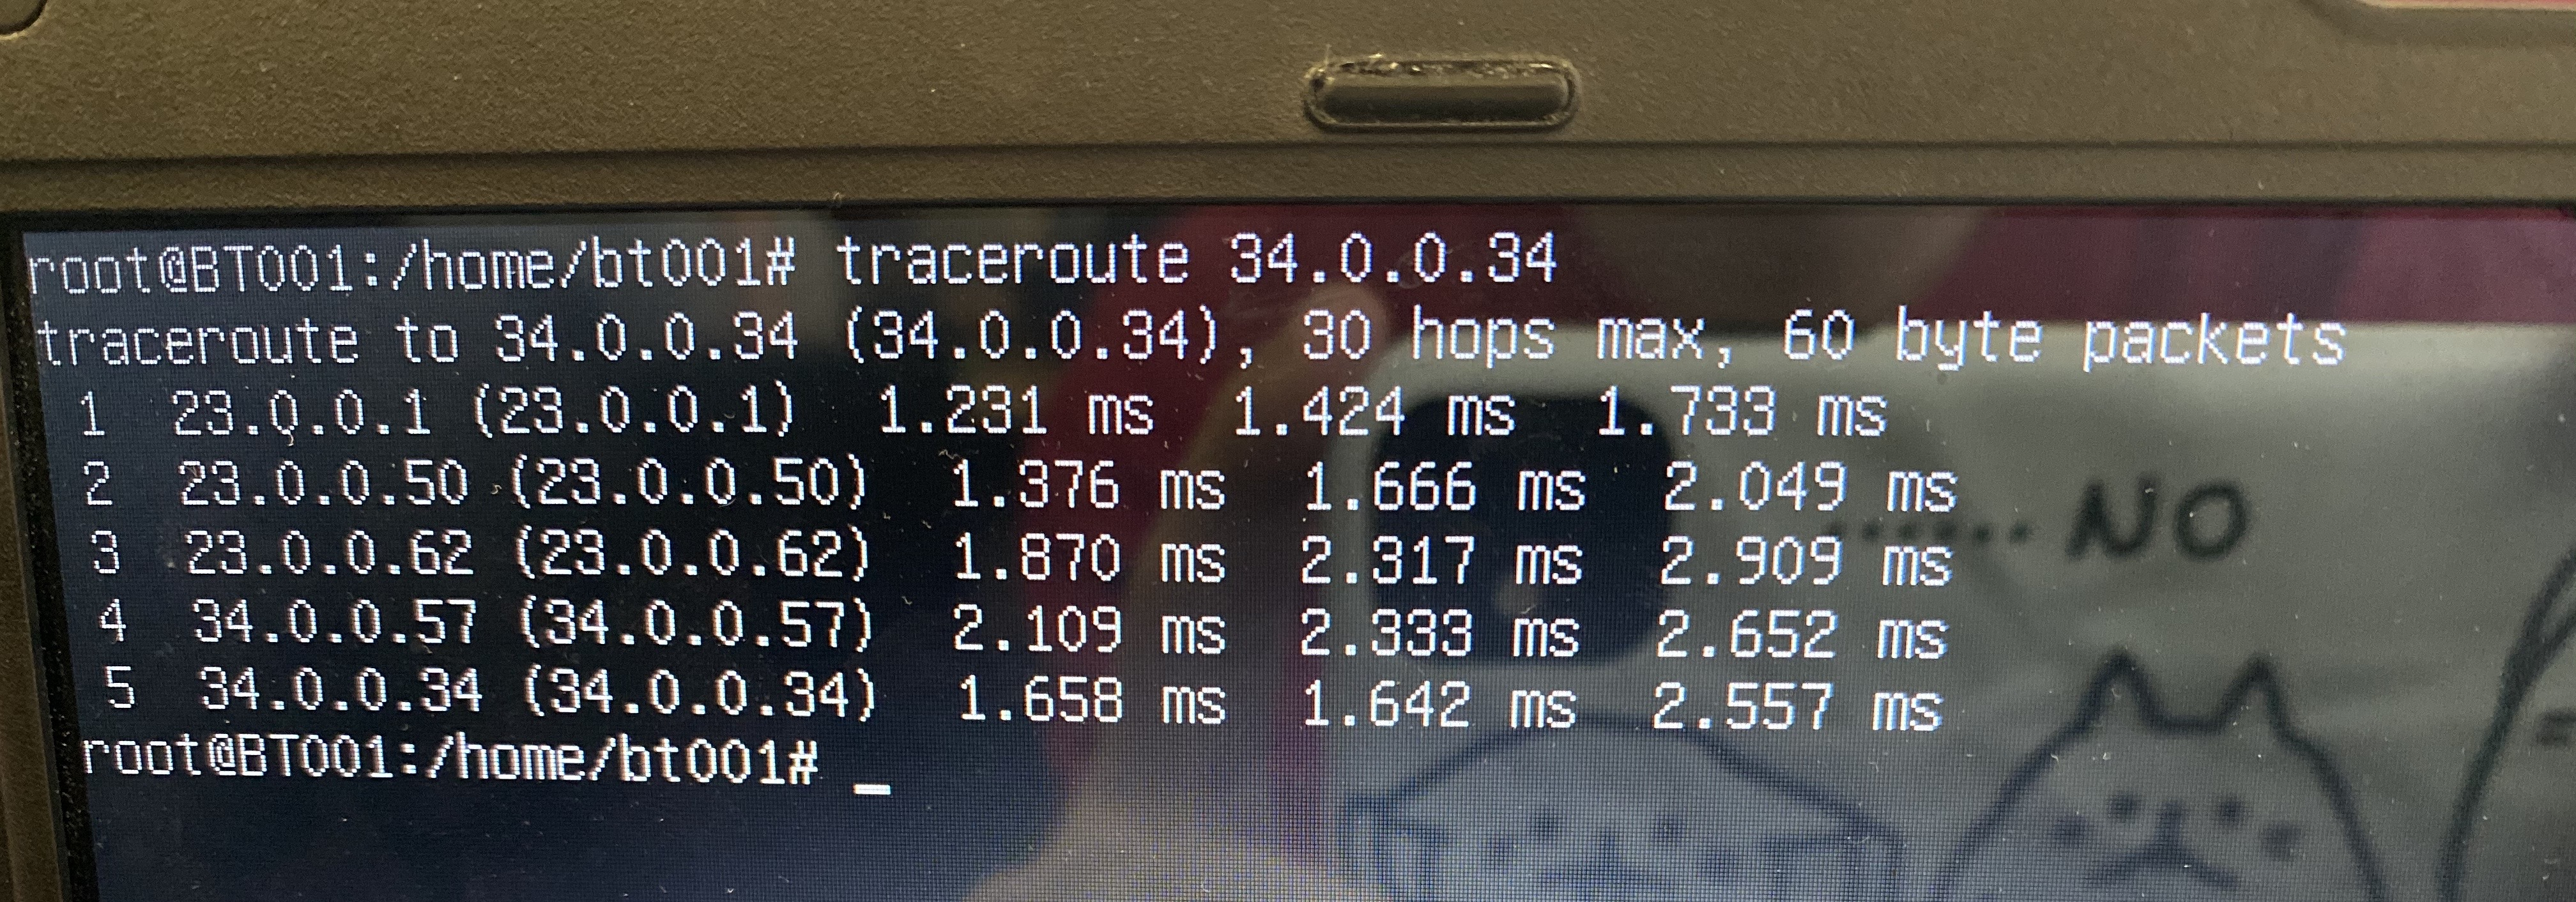
\includegraphics[width=\linewidth]{bgp-dt-3}
        \caption{\texttt{34.0.0.34}}
    \end{subfigure}
    ~
    \caption{Tracing IPv4 Routes to DT Network on Laptop 1 (BT001) using \texttt{traceroute}.}
    \label{fig:bgp-dt}
\end{figure*}



\clearpage

\subsubsection{Connectivity to Peer Virgin Network}
The connectivity to peer Virgin Network using BGP protocol is tested and evaluated by tracing routes to IP addresses \texttt{56.0.0.2}, \texttt{56.0.0.18} and \texttt{56.0.0.34} on Laptop 1 (BT001). As shown in Figure \ref{fig:bgp-virgin}, connection to Virgin Network is successfully established through BGP routes.

\begin{figure*}[ht!]
    \centering
    \begin{subfigure}[b]{\textwidth}
        \centering
        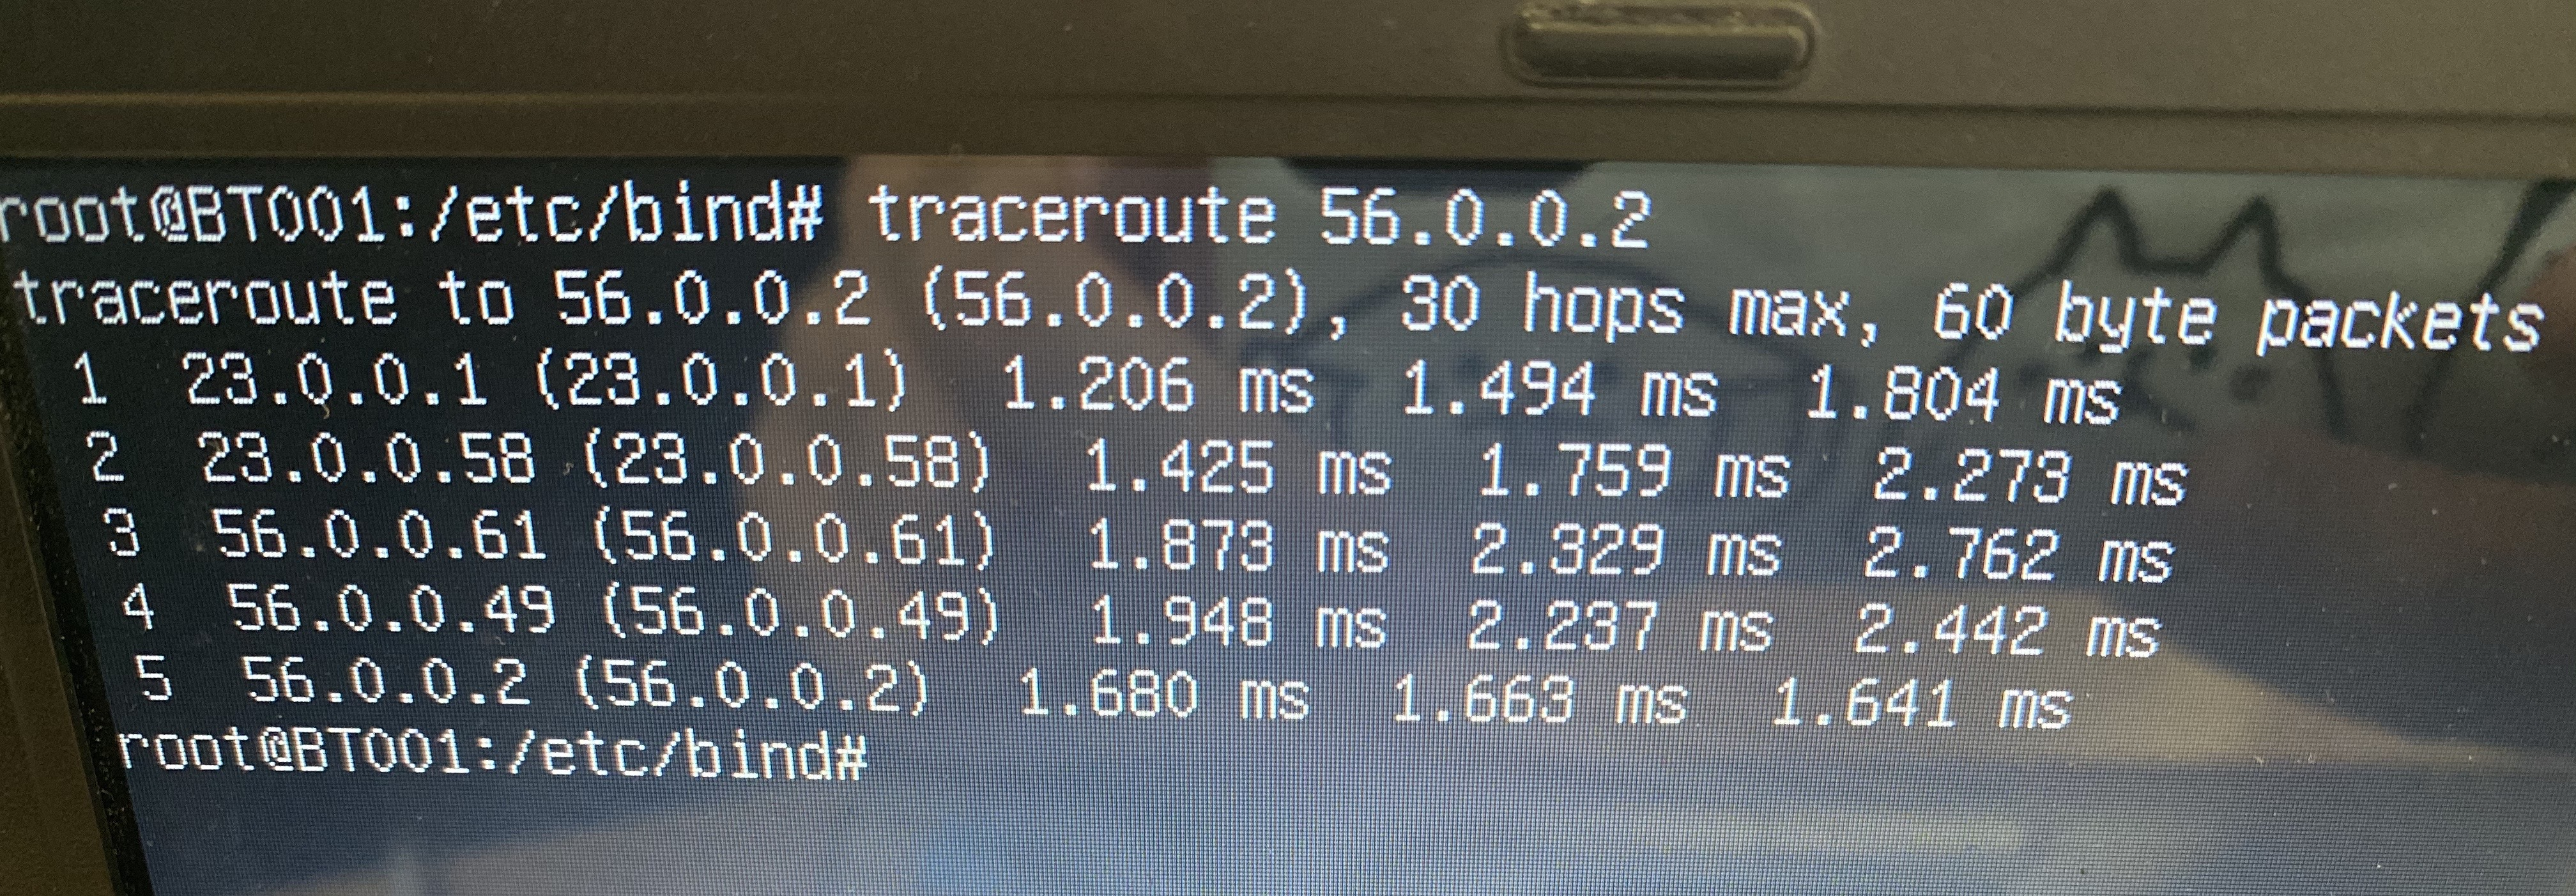
\includegraphics[width=\linewidth]{bgp-virgin-1}
        \caption{\texttt{56.0.0.2}}
    \end{subfigure}
    ~
    \begin{subfigure}[b]{\textwidth}
        \centering
        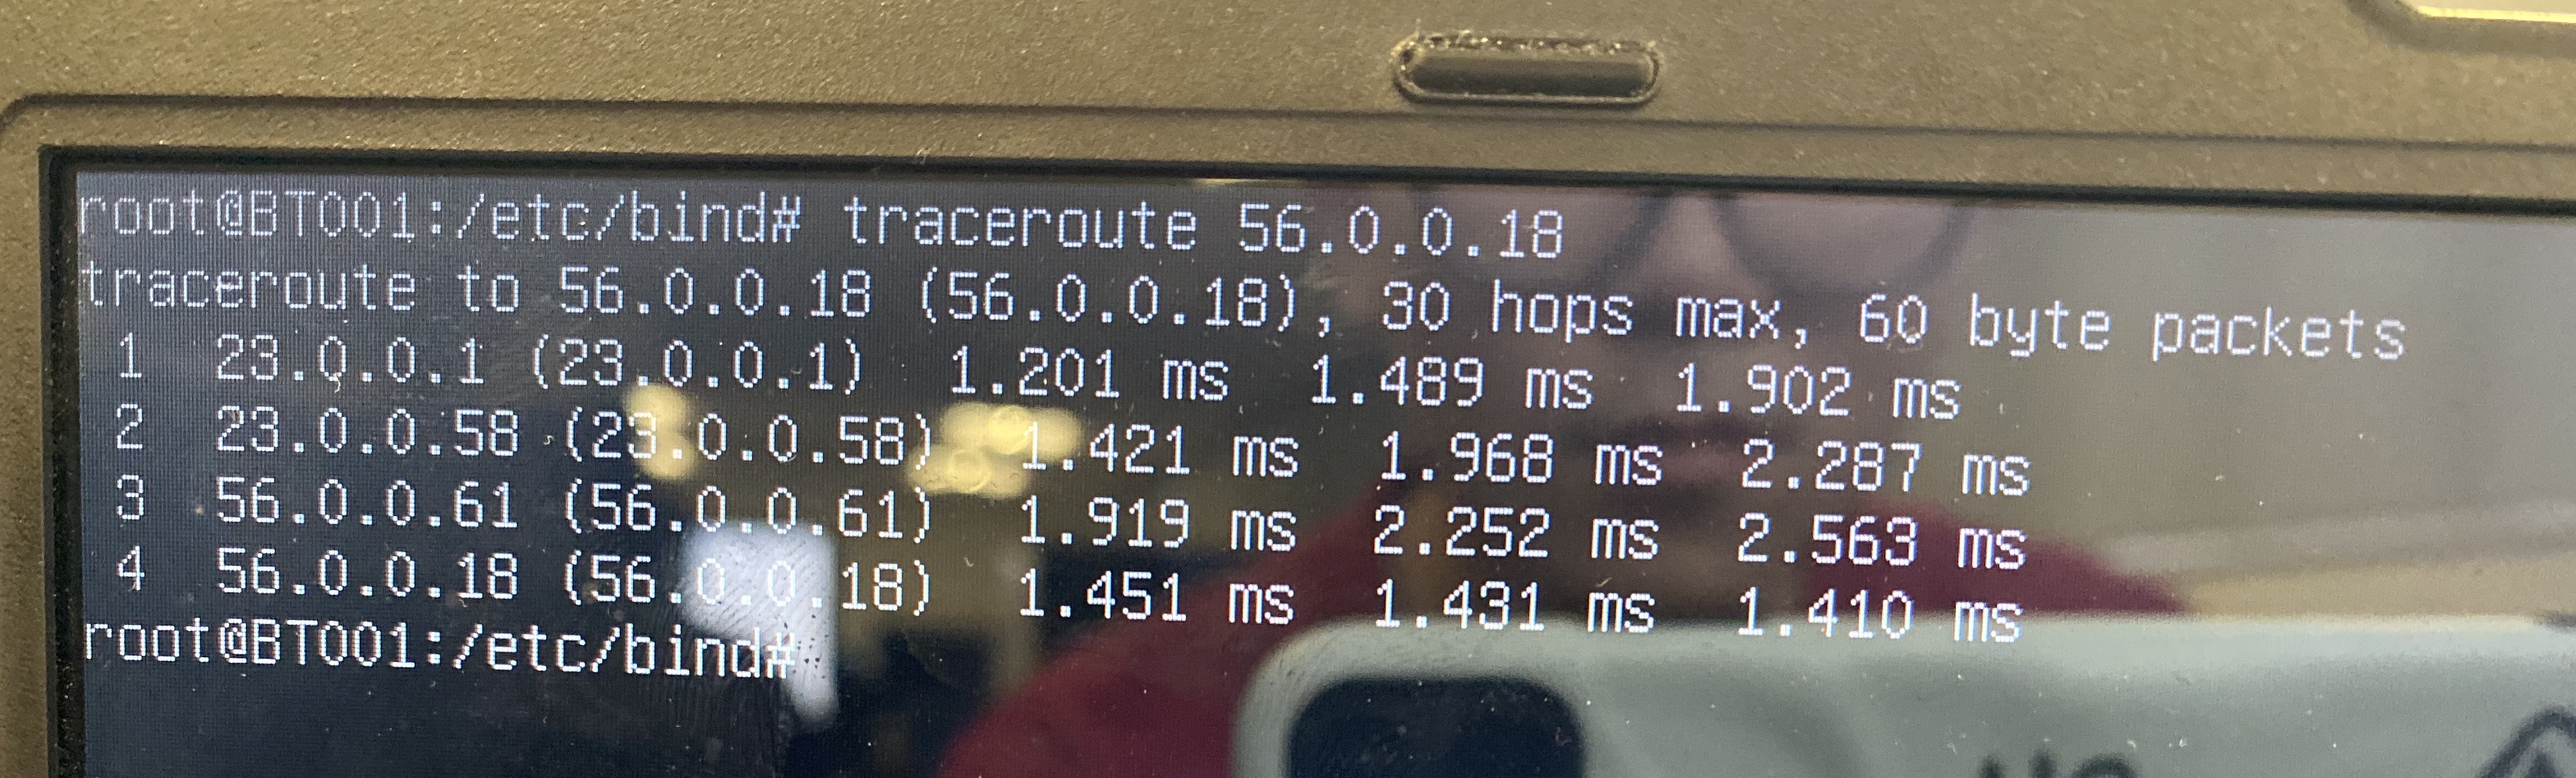
\includegraphics[width=\linewidth]{bgp-virgin-2}
        \caption{\texttt{56.0.0.18}}
    \end{subfigure}
    ~
    \begin{subfigure}[b]{\textwidth}
        \centering
        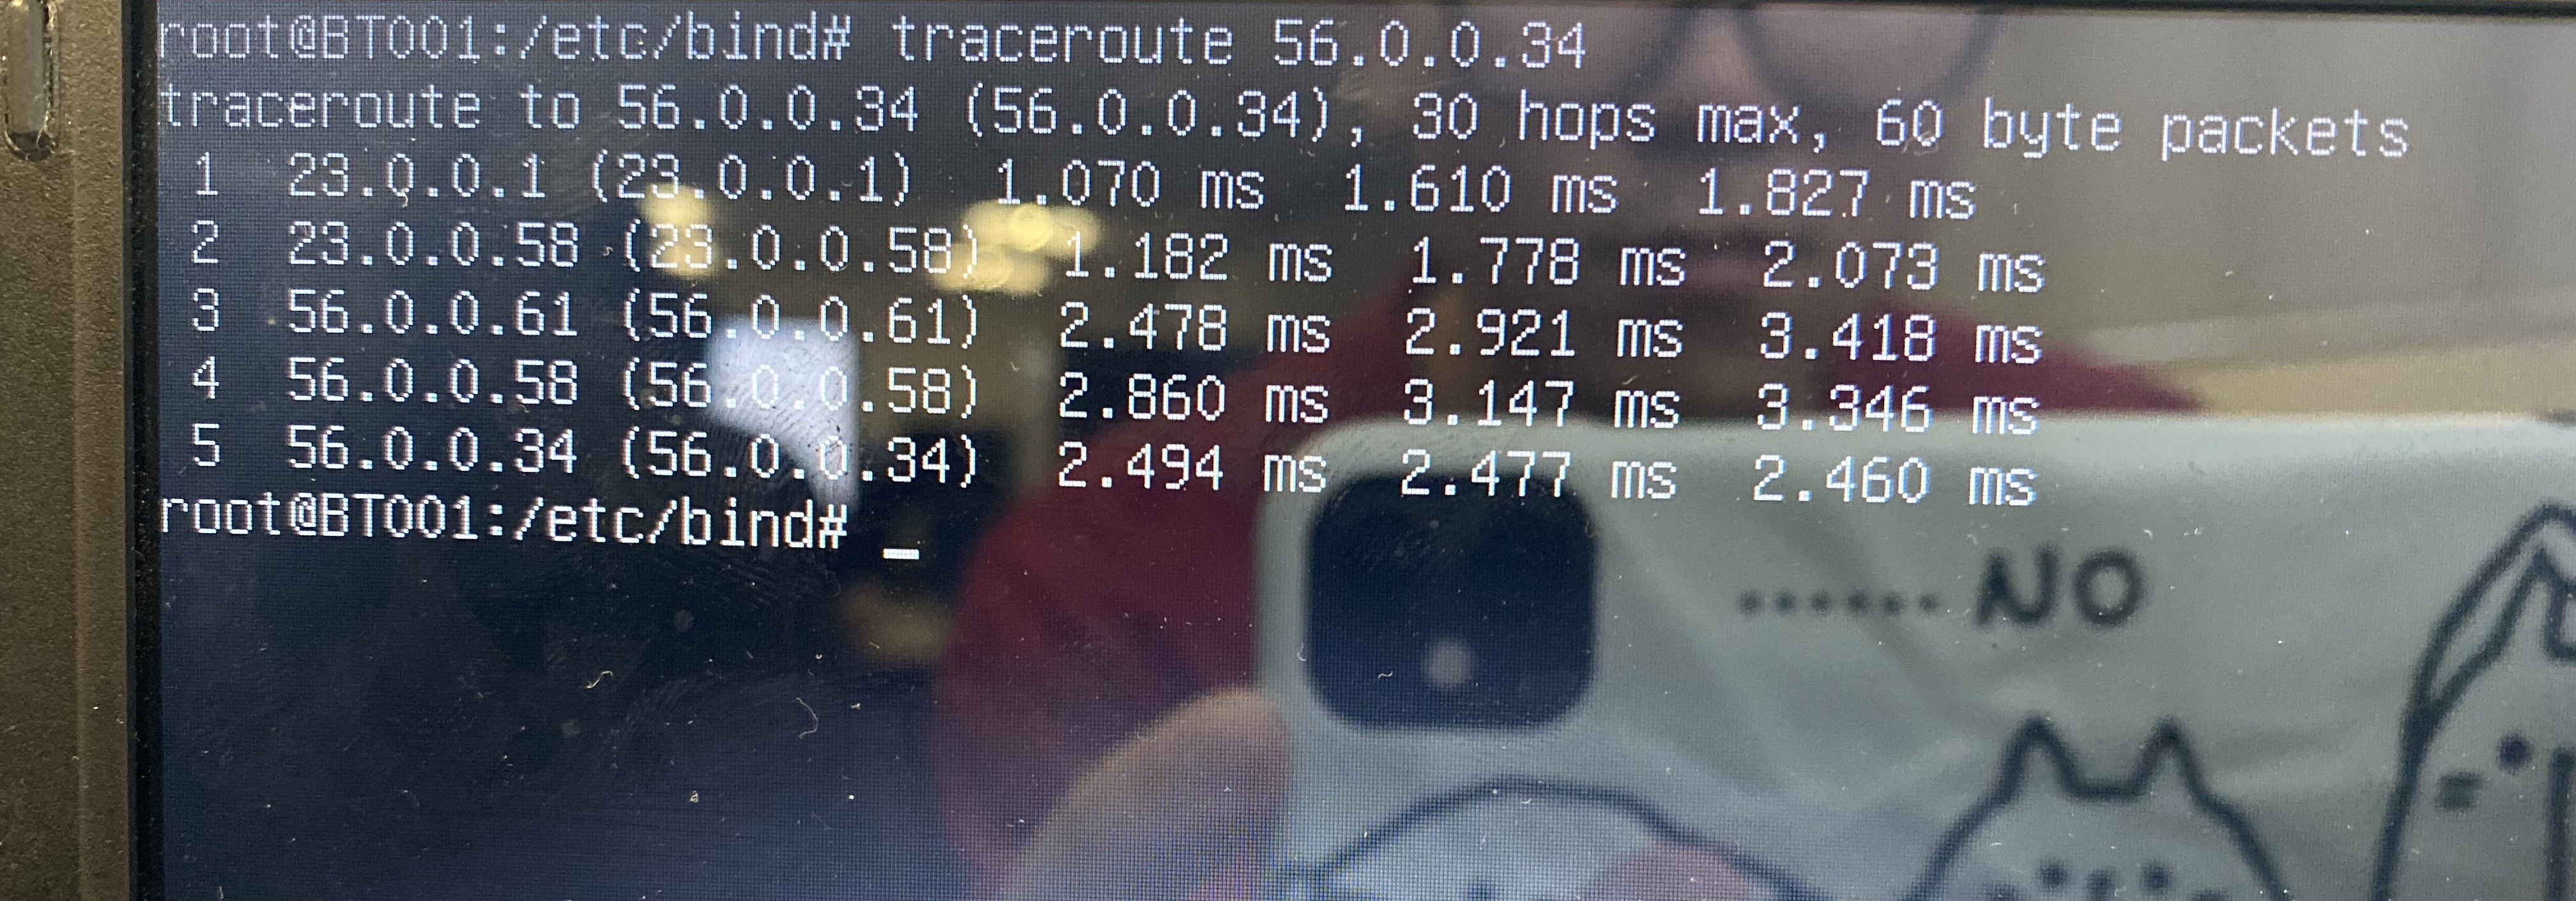
\includegraphics[width=\linewidth]{bgp-virgin-3}
        \caption{\texttt{56.0.0.34}}
    \end{subfigure}
    ~
    \caption{Tracing IPv4 Routes to Virgin Network on Laptop 1 (BT001) using \texttt{traceroute}.}
    \label{fig:bgp-virgin}
\end{figure*}



\clearpage


\subsubsection{Connectivity to Other Networks}
The connectivity to other networks using BGP protocol is tested and evaluated by tracing routes to IP addresses \texttt{78.0.0.2} (Sonara Network) and \texttt{89.0.0.18} (NTT Network) on Laptop 1 (BT001). As shown in Figure \ref{fig:bgp-virgin}, connection to Virgin Network is successfully established through BGP routes.

\begin{figure*}[ht!]
    \centering
    \begin{subfigure}[b]{\textwidth}
        \centering
        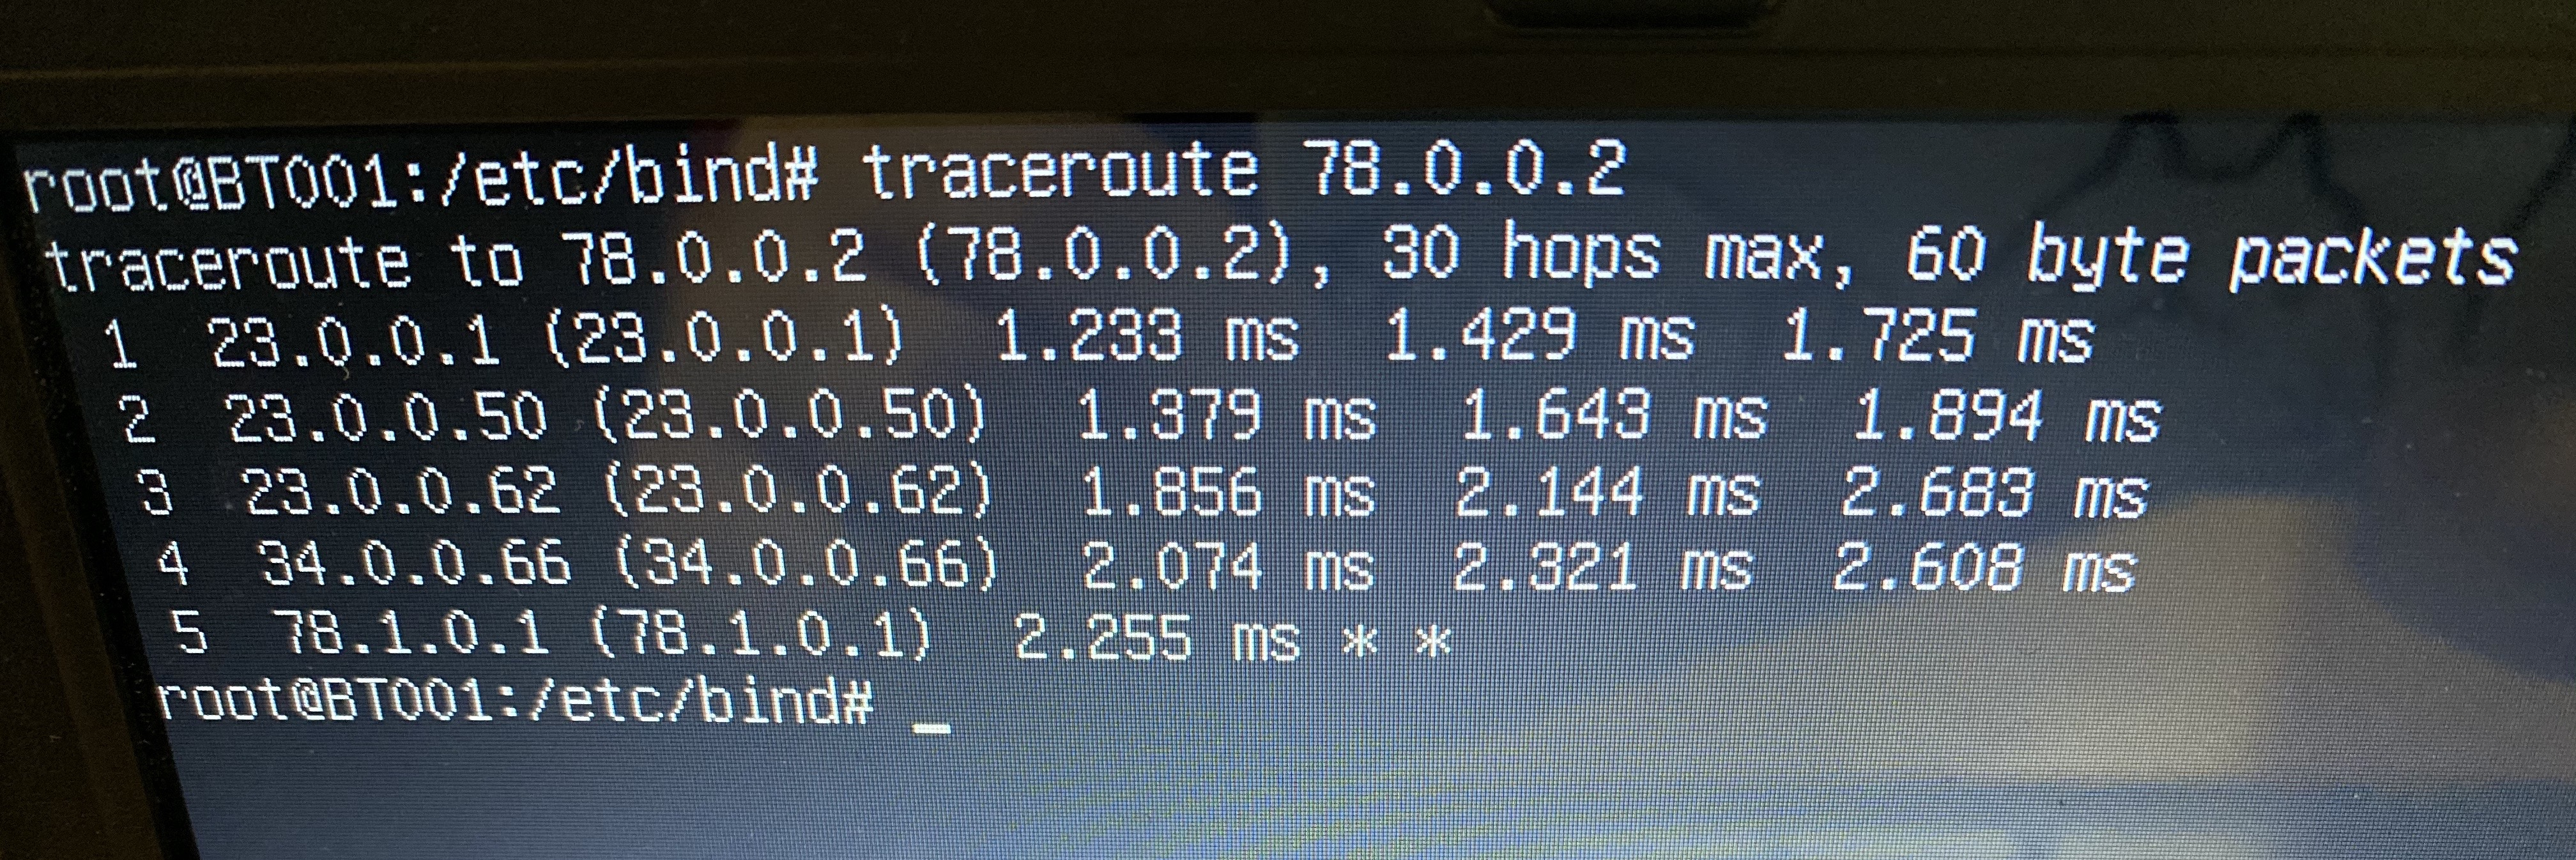
\includegraphics[width=\linewidth]{bgp-other-1}
        \caption{\texttt{78.0.0.2}}
    \end{subfigure}
    ~
    \begin{subfigure}[b]{\textwidth}
        \centering
        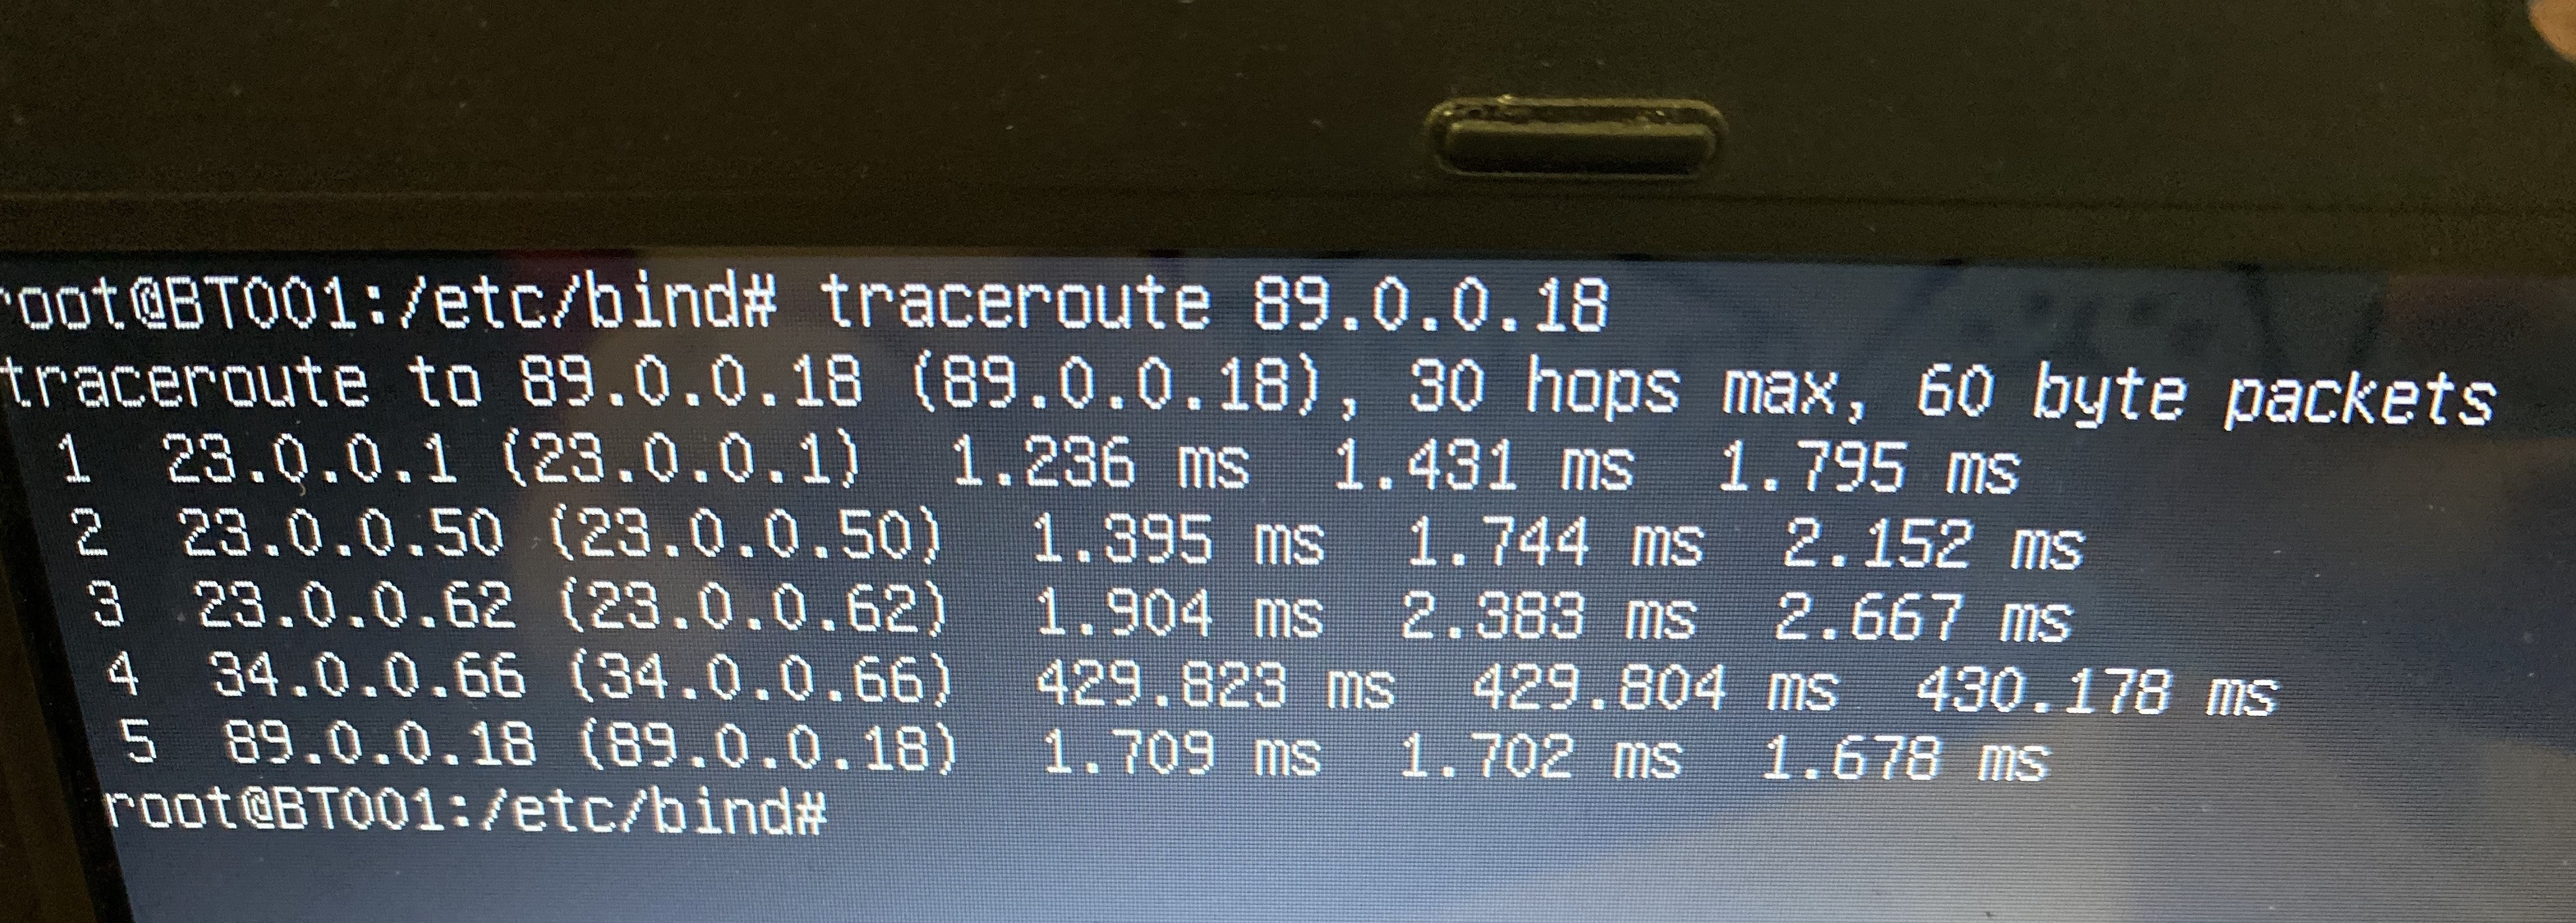
\includegraphics[width=\linewidth]{bgp-other-2}
        \caption{\texttt{89.0.0.18}}
    \end{subfigure}
    \caption{Tracing IPv4 Routes to Other Networks on Laptop 1 (BT001) using \texttt{traceroute}.}
    \label{fig:bgp-virgin}
\end{figure*}



\clearpage

\subsubsection{Connectivity to Virgin when Direct Physical Connection Is Down}
In addition, the connectivity to peer Virgin Network under the unfortunate condition that the direct physical connection is down is also tested. 
Traced routes to IP addresses \texttt{56.0.0.2}, \texttt{56.0.0.18} and \texttt{56.0.0.34} on Laptop 1 (BT001) are shown in Figure \ref{fig:bgp-virgin-broken}.

Alternative connection to Virgin Network is successfully established through Central Network (ASN: 42).

\begin{figure*}[ht!]
    \centering
    \begin{subfigure}[b]{\textwidth}
        \centering
        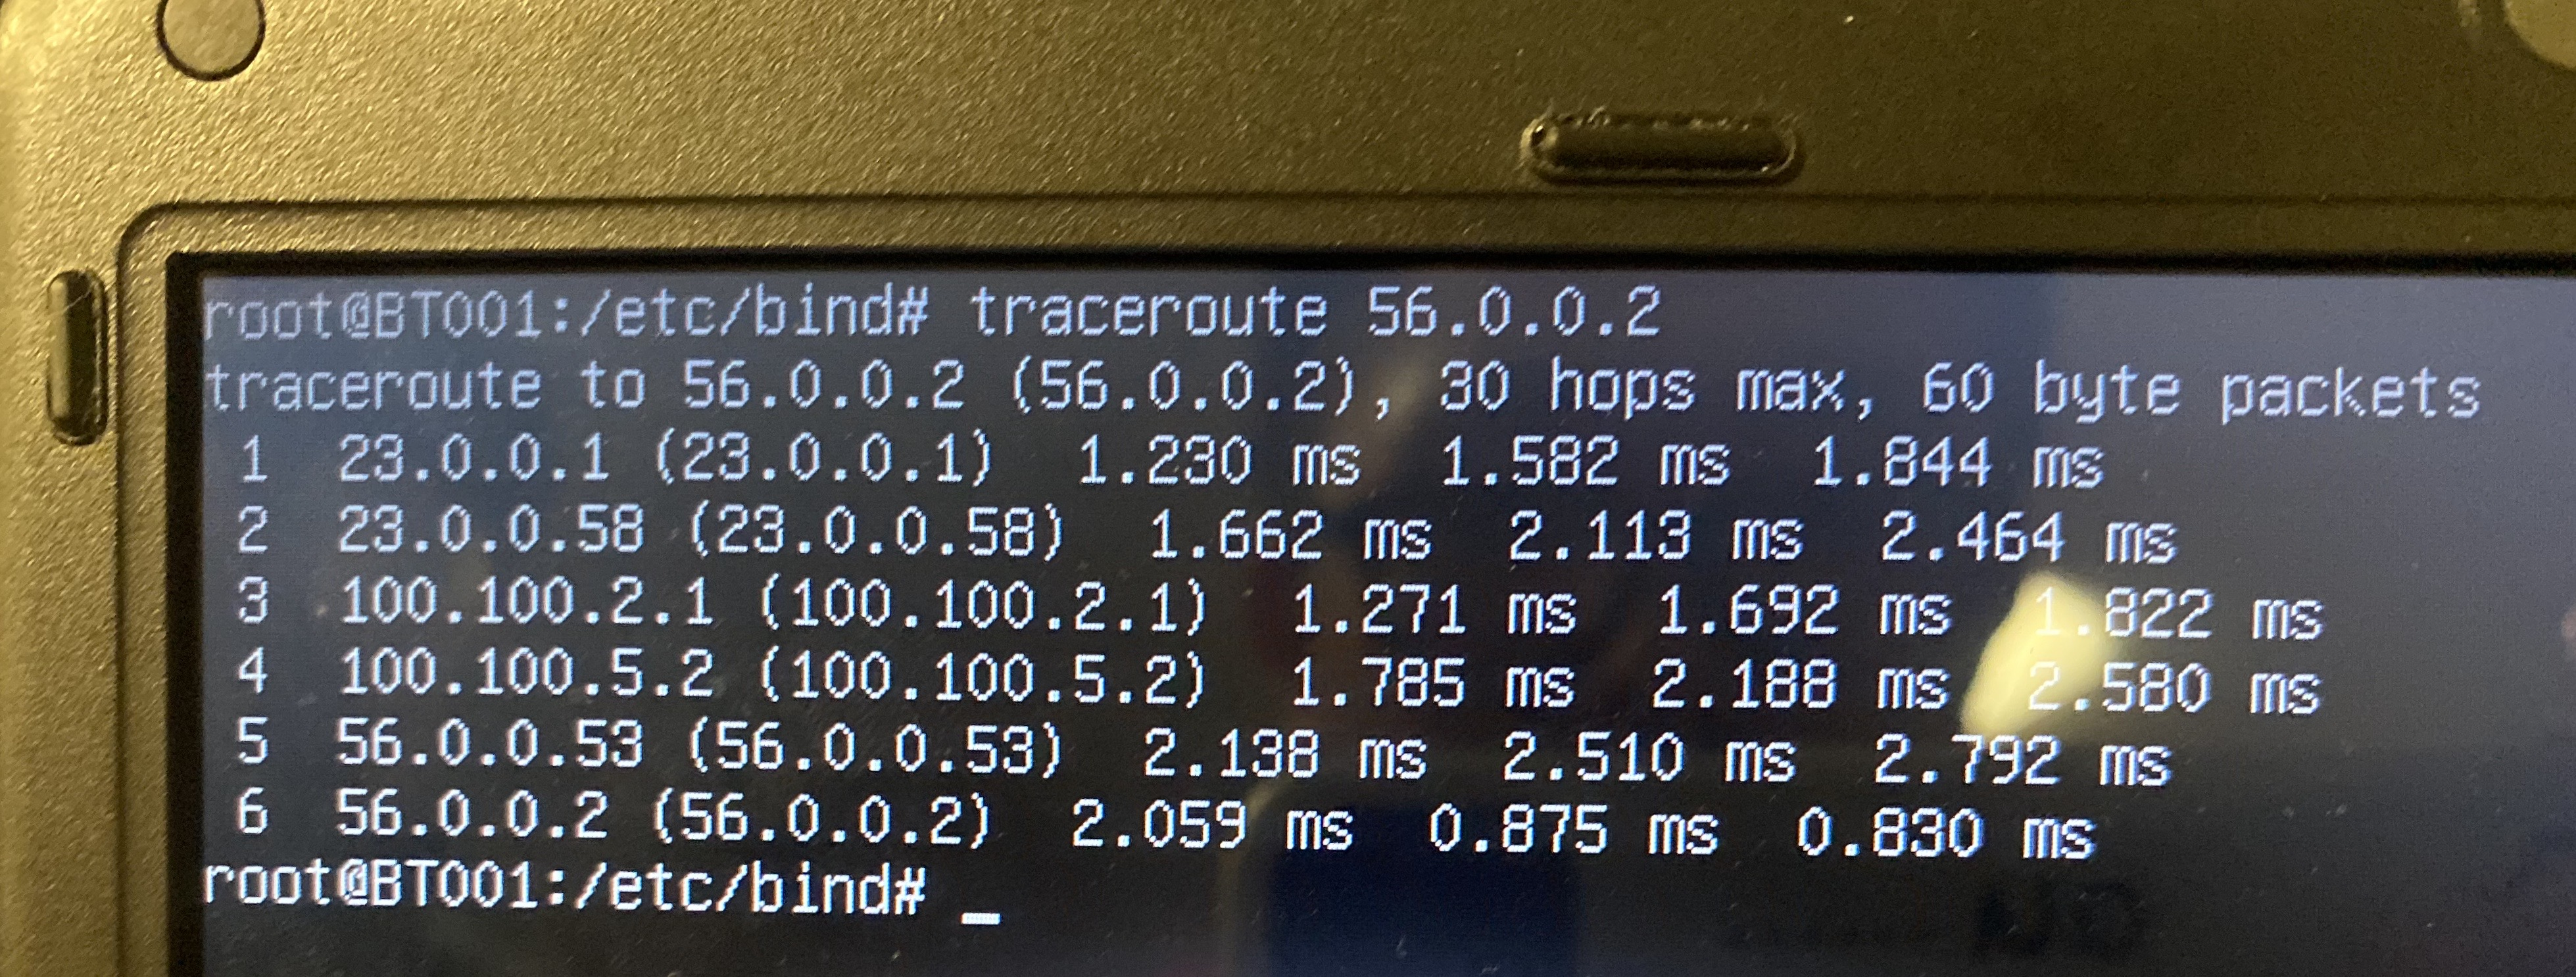
\includegraphics[width=\linewidth]{bgp-virgin-broken-1}
        \caption{\texttt{56.0.0.2}}
    \end{subfigure}
    ~
    \begin{subfigure}[b]{\textwidth}
        \centering
        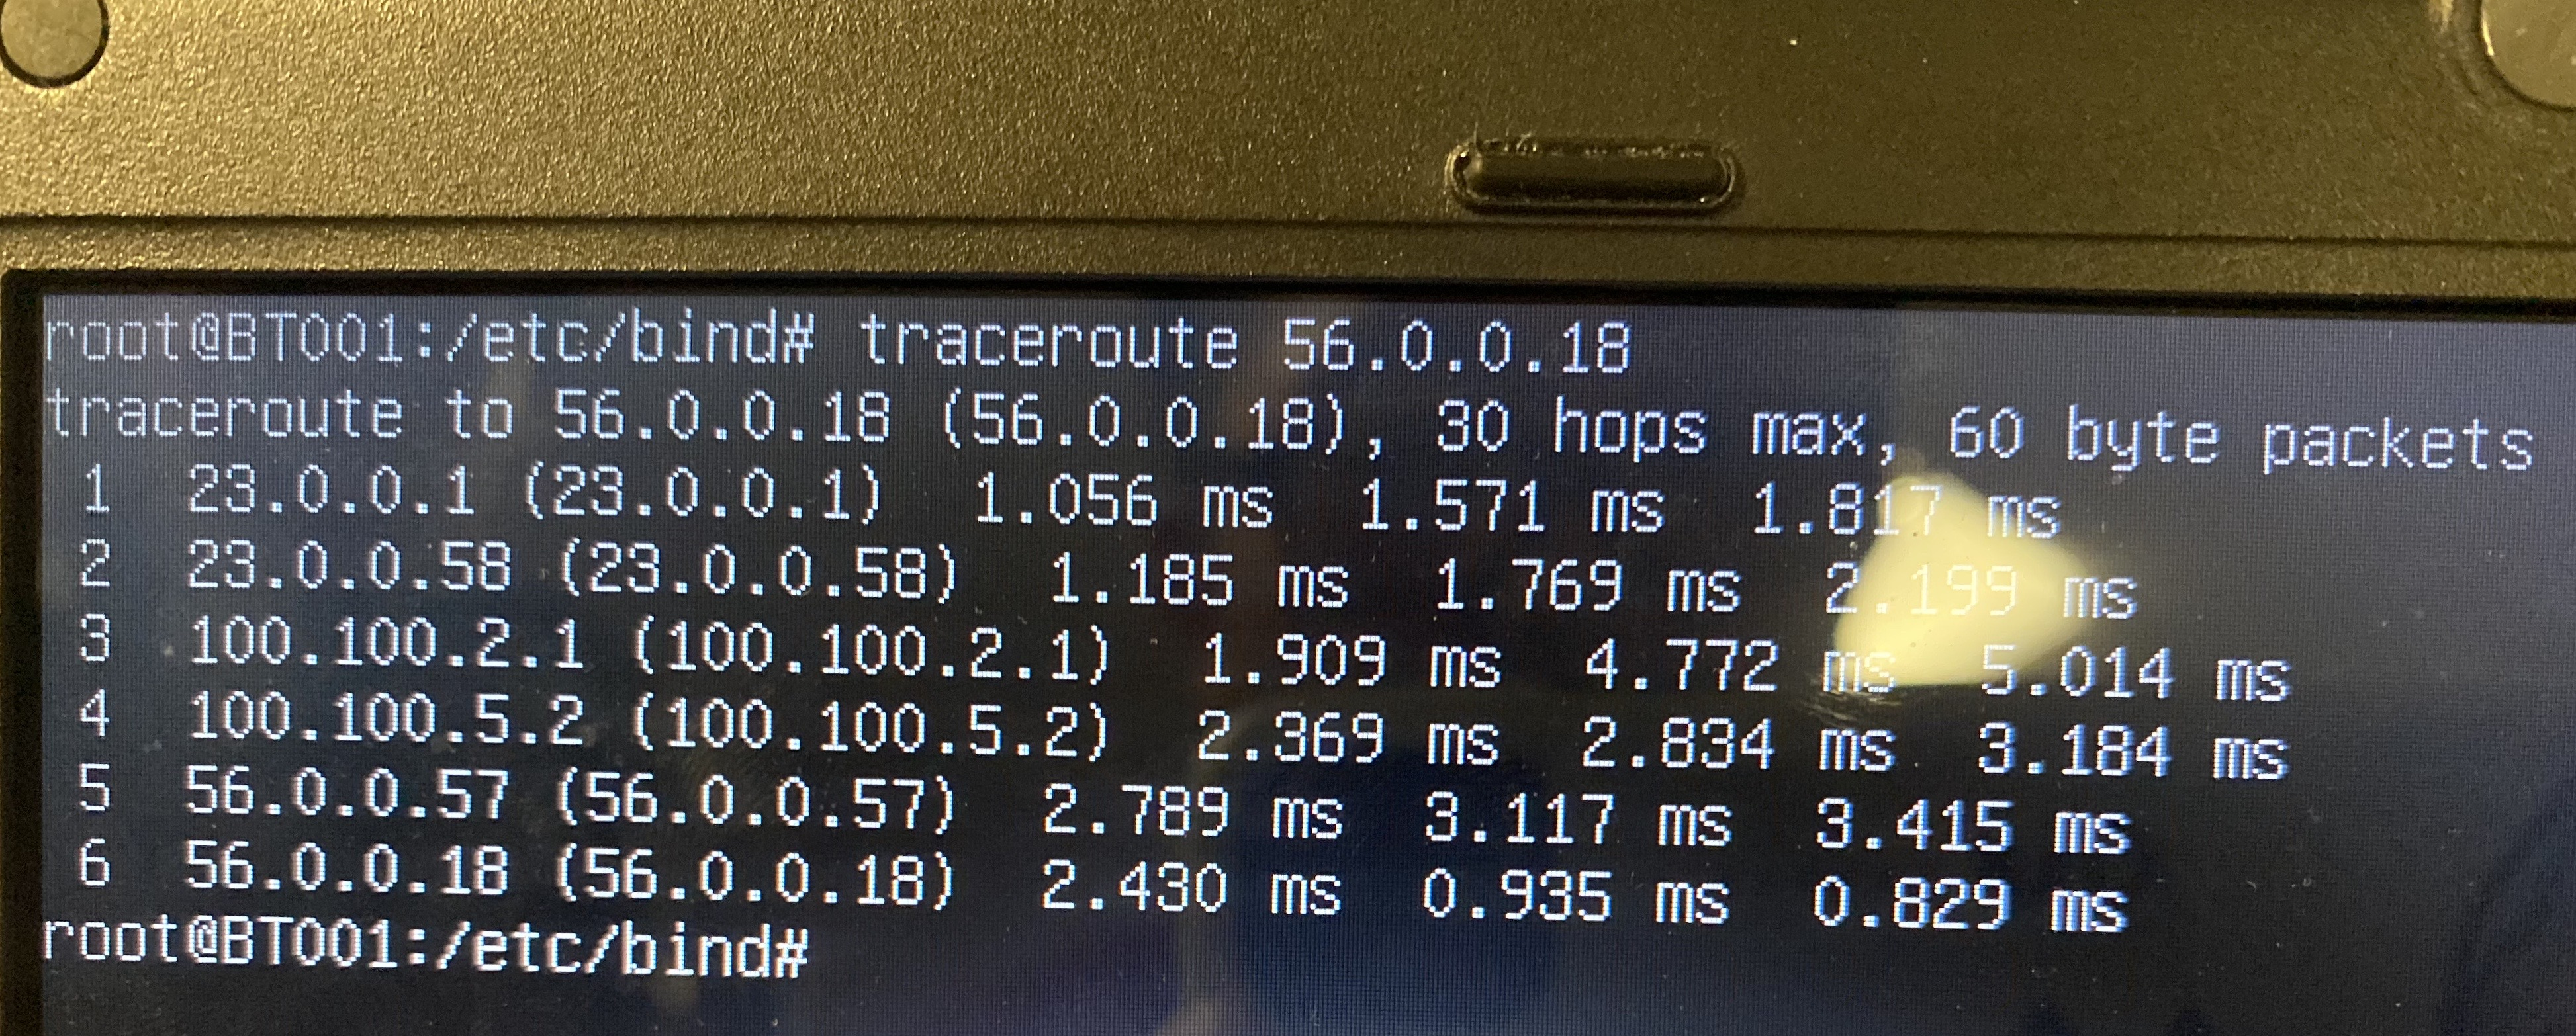
\includegraphics[width=\linewidth]{bgp-virgin-broken-2}
        \caption{\texttt{56.0.0.18}}
    \end{subfigure}
    ~
    \begin{subfigure}[b]{\textwidth}
        \centering
        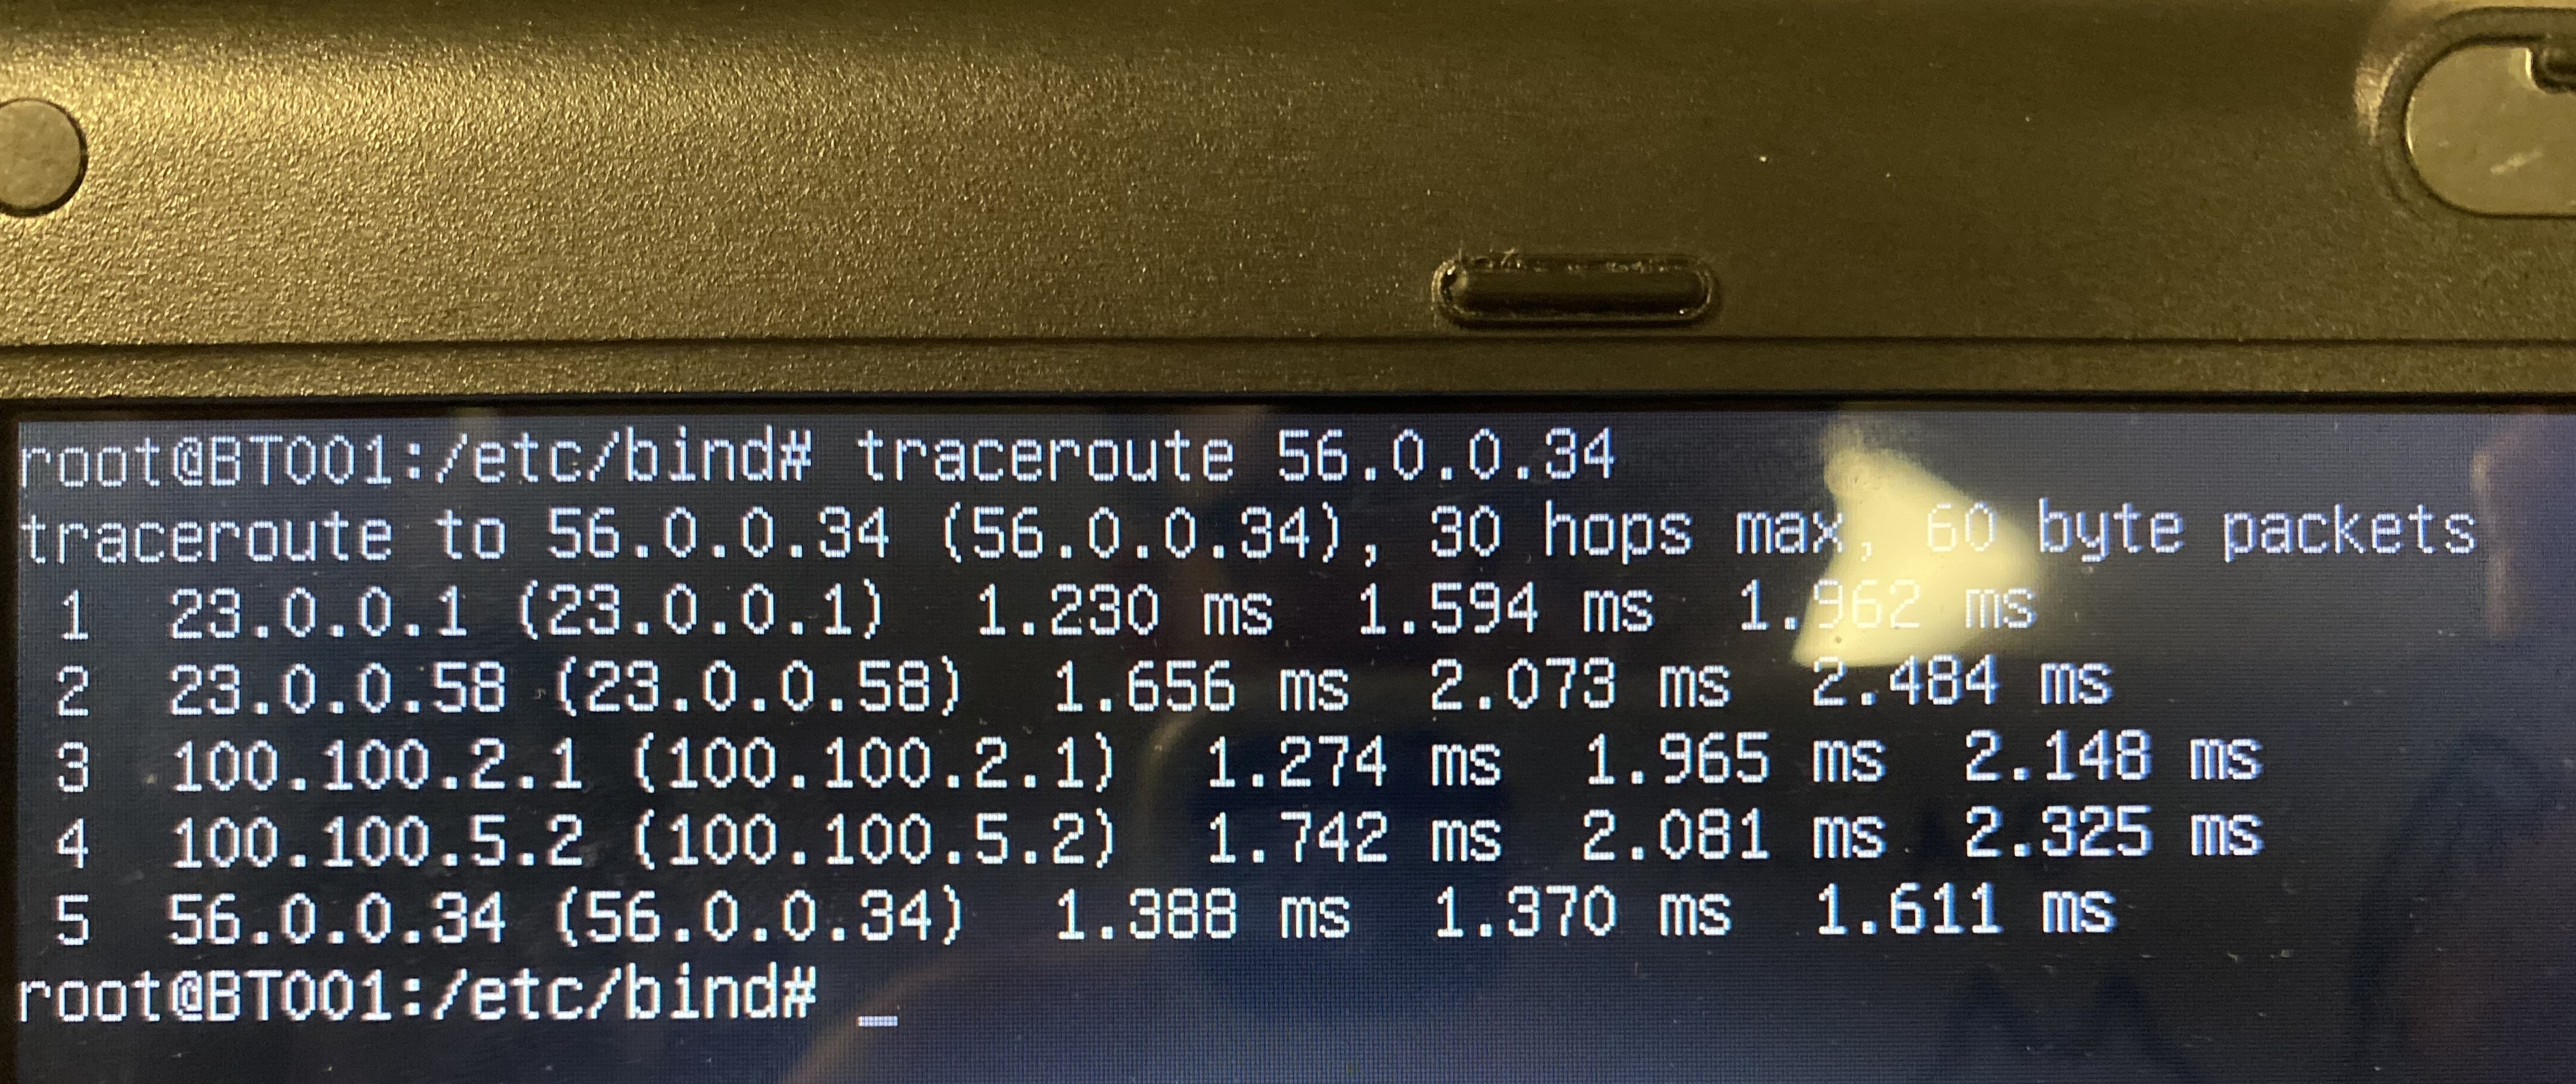
\includegraphics[width=\linewidth]{bgp-virgin-broken-3}
        \caption{\texttt{56.0.0.34}}
    \end{subfigure}
    ~
    \caption{Tracing IPv4 Routes to Virgin Network on Laptop 1 (BT001) using \texttt{traceroute} When Direct Physical Connection Is Broken .}
    \label{fig:bgp-virgin-broken}
\end{figure*}


\subsection{Commentary}

\subsubsection{Problem: Filter List Not Working for Self-Originated Routes}

The initial filter list for outbound routes on Router 3 only permits routes originated from BT Network (ASN 2030) and customer DT Network (ASN 3040).

\begin{lstlisting}
ip as-path access-list 1 permit _2030$
ip as-path access-list 1 permit _3040$
\end{lstlisting}

However, the filter list blocks all routes except those originated from customer DT Network to be announced. To solve this problem, a filter list where all routes except those go through provider Central Network (ASN 42) and peer Virgin Network (ASN 5060) are allowed. The new list should have the same effects as the previous list and indeed works as intended.

\begin{lstlisting}
ip as-path access-list 1 deny _42_
ip as-path access-list 1 deny _5060_
ip as-path access-list 1 permit .*
\end{lstlisting}

% \subsubsection{Problem: Loopback Addresses}




\newpage


\chapter{Applications in the Network}
\label{chap:applications}

\section{Secure Remote Access to Routers through SSH}

\subsection{Design}

Accessing the routers through the physical "console" port is inconvenient and dangerous. Thus, remote acess through Secure Shell (SSH) protocol to routers is needed. 

In our network, we enable remote SSH access on all 3 routers. We use seperate combinations of username and password on each router to ensure the independence of security of each router.

In addition, we set up SSH public key authentication on Laptop 1 (BT001), which allows the root user on the laptop to login in to all routers without entering passwords.

\subsection{Implementation}

We first set up remote SSH access as instructed in Reference Guide on all 3 routers. Below is the configuration commands for Router 1 (BT-R001).

\begin{lstlisting}
hostname BT-R001
ip domain name bt.lboro
username r001 priv 15 secret <secret>
line vty 0 4
transport input ssh telnet
login local

ip ssh version 2
crypto key generate rsa general-keys
ip ssh dh min size 4096
\end{lstlisting}

We then generate a pair of public and private keys on Laptop 1 (BT001).

\begin{lstlisting}
ssh-keygen
\end{lstlisting}

After that, the pair of keys is written into files
\texttt{\textasciitilde{}/.ssh/id\_rsa} and
\texttt{\textasciitilde{}/.ssh/id\_rsa.pub} . We use the generated
public key ( \texttt{id\_rsa.pub} ) to set up SSH public key
authentication on all 3 routers.

\begin{lstlisting}
ip ssh pubkey-chain
username r001
key-string
\end{lstlisting}

\subsection{Evaluation}

Once remote SSH access is set up on 3 routers, we should be able to access them on Laptop 1 (BT001) without entering the password using the following commands.

\begin{lstlisting}[language=sh]
# access Router 1
ssh r001@23.0.0.1 
# access Router 2
ssh r002@23.0.0.50
# access Router 3
ssh r003@23.0.0.33
\end{lstlisting}

Screenshots of successful remote access to all 3 routers are shown in Figure \ref{fig:ssh}.

\begin{figure*}[t!]
    \centering
    \begin{subfigure}[t]{0.3\textwidth}
        \centering
        \includegraphics[width=\linewidth]{ssh1}
        \caption{Router 1 (BT-R001)}
    \end{subfigure}
    ~ 
    \begin{subfigure}[t]{0.3\textwidth}
        \centering
        \includegraphics[width=\linewidth]{ssh2}
        \caption{Router 2 (BT-R002)}
    \end{subfigure}
    ~ 
    \begin{subfigure}[t]{0.3\textwidth}
        \centering
        \includegraphics[width=\linewidth]{ssh3}
        \caption{Router 3 (BT-R003)}
    \end{subfigure}
    \caption{Sucessful remote SSH access to all 3 routers from Laptop 1 (BT001).}
    \label{fig:ssh}
\end{figure*}


\subsection{Commentary}

\subsubsection{Problem: Maximum Limit of Characters per Line}

When we tried to set up SSH public key authentication on routers, we failed at our initial attempt. It turned out that Cisco router has maximum limit of characters for each command line. Thus, a public key in a single long line was not accepted by the router. 

To solve this problem, we then used \texttt{fold} command to split the public key into multiple lines before re-uploading the key and SSH public key authentication was successfully set up on the router.


\section{World Wide Web Service}

\subsection{Design}

\subsection{Implementation}

\subsection{Evaluation}

\subsection{Commentary}



\section{Domain Name System Service}

\subsection{Design}

\subsection{Implementation}

\subsection{Evaluation}

\subsection{Commentary}


\section{Email Service}

\subsection{Design}

\subsection{Implementation}

\subsection{Evaluation}

\subsection{Commentary}

\section{Secure Remote Access to Routers through SSH}
\label{sec:ssh}

\subsection{Design}

Accessing the routers through the physical "console" port is inconvenient and dangerous. Thus, remote acess through Secure Shell (SSH) protocol to routers is needed. 

In BT network, remote SSH access is enabled on all 3 routers. Seperate combinations of username and password on each router are used to ensure the independence of security of each router.

In addition, SSH public key authentication is set up on Laptop 1 (BT001), which allows the root user on the laptop to login in to all routers without entering passwords.

\subsection{Implementation}

We first set up Remote SSH access was first set up as instructed in Reference Guide on all 3 routers. Below is the configuration commands for Router 1 (BT-R001).

\begin{lstlisting}
hostname BT-R001
ip domain name bt.lboro
username r001 priv 15 secret <secret>
line vty 0 4
transport input ssh telnet
login local

ip ssh version 2
crypto key generate rsa general-keys
ip ssh dh min size 4096
\end{lstlisting}

We then generate a pair of public and private keys on Laptop 1 (BT001).

\begin{lstlisting}
ssh-keygen
\end{lstlisting}

After that, the pair of keys is written into files
\texttt{\textasciitilde{}/.ssh/id\_rsa} and
\texttt{\textasciitilde{}/.ssh/id\_rsa.pub} . We use the generated
public key ( \texttt{id\_rsa.pub} ) to set up SSH public key
authentication on all 3 routers.

\begin{lstlisting}
ip ssh pubkey-chain
username r001
key-string
\end{lstlisting}

\subsection{Evaluation}

Once remote SSH access is set up on 3 routers, one should be able to access them on Laptop 1 (BT001) without entering the password using the following commands.

\begin{lstlisting}[language=sh]
# access Router 1
ssh r001@23.0.0.1 
# access Router 2
ssh r002@23.0.0.50
# access Router 3
ssh r003@23.0.0.33
\end{lstlisting}

Screenshots of successful remote access to all 3 routers are shown in Figure \ref{fig:ssh}.

\begin{figure*}[ht!]
    \centering
    \begin{subfigure}[b]{0.67\textwidth}
        \centering
        \includegraphics[width=\linewidth]{ssh1}
        \caption{Router 1 (BT-R001)}
    \end{subfigure}
    \hfill
    \begin{minipage}[b]{0.3\textwidth}
	    \begin{subfigure}[b]{\linewidth}
	        \centering
	        \includegraphics[width=\linewidth]{ssh2}
	        \caption{Router 2 (BT-R002)}
	    \end{subfigure}
	    \\
	    \begin{subfigure}[b]{\linewidth}
	        \centering
	        \includegraphics[width=\linewidth]{ssh3}
	        \caption{Router 3 (BT-R003)}
	    \end{subfigure}
	\end{minipage}
    \caption{Sucessful remote SSH access to all 3 routers from Laptop 1 (BT001).}
    \label{fig:ssh}
\end{figure*}

% \begin{figure*}[t!]
%     \centering
%     \begin{subfigure}[t]{0.3\textwidth}
%         \centering
%         \includegraphics[width=\linewidth]{ssh1}
%         \caption{Router 1 (BT-R001)}
%     \end{subfigure}
%     ~ 
%     \begin{subfigure}[t]{0.3\textwidth}
%         \centering
%         \includegraphics[width=\linewidth]{ssh2}
%         \caption{Router 2 (BT-R002)}
%     \end{subfigure}
%     ~ 
%     \begin{subfigure}[t]{0.3\textwidth}
%         \centering
%         \includegraphics[width=\linewidth]{ssh3}
%         \caption{Router 3 (BT-R003)}
%     \end{subfigure}
%     \caption{Sucessful remote SSH access to all 3 routers from Laptop 1 (BT001).}
%     \label{fig:ssh}
% \end{figure*}


\subsection{Commentary}

\subsubsection{Problem: Maximum Limit of Characters per Line}

When we tried to set up SSH public key authentication on routers, we failed at our initial attempt. It turned out that Cisco router has maximum limit of characters for each command line. Thus, a public key in a single long line was not accepted by the router. 

To solve this problem, \texttt{fold} command is used to split the public key into multiple lines before re-uploading the key and SSH public key authentication was successfully set up on the router.

\newpage
\section{Domain Name System Service}
\label{sec:dns}

\subsection{Design}

Domain Name System (DNS)\citep{rfc1035} translates IP addresses to domain names and vice versa.
In contrast to hard-to-remember IP addresses, short and meaningful domain names (eg. \texttt{lboro.ac.uk} for Loughborough University in UK) are more convient for Internet users. 
Additionally, the service providers can change the IP addresses of servers without re-notifying their customers.

In BT Network, there are two DNS servers, one primary master server and the other secondary. Primary master server is deployed at Laptop 3 (BT003) and secondary master server is at Laptop 1 (BT001). 
The rationale is that when the primary becomes unavailable, the secondary can be the backup domain name server.

Both are authoritative of domain \texttt{bt.lboro}. \textbf{Each laptop in the network has a corresponding domain name. For example, the domain name of Laptop 1 (BT001) is \texttt{bt001.bt.lboro}. In addition, both \texttt{A} and \texttt{AAAA} records of \texttt{bt.lboro} point to Laptop 1 while the MX record points to Laptop 3.}

The two DNS servers are also connected to the central DNS server, which is authoritative of domain \texttt{lboro}.



\subsection{Implementation}

Install \texttt{bind9} package and \texttt{dnsutils} package on Laptop 1 (BT001) and Laptop 3 (BT001) using the following commands. All DNS configurations are all stored in folder \texttt{/etc/bind}.

\begin{lstlisting}
sudo apt-get install bind9
sudo apt-get install dnsutils
\end{lstlisting}


On the primary DNS server, forward unknown DNS requests to central DNS server by adding this line to file \texttt{named.conf.options}.

\begin{lstlisting}
forwarders { 10.2.2.1; };
\end{lstlisting}



The following lines are added to file \texttt{/etc/bind/named.conf.local}.

The zone section defines the type of the DNS server and it is stored in a file mentioned in the 'file' field. 
The 'allow-transfer' field defines a match list which has IP addresses that are allowed to do transfer and copy operations to the zone information with the server. 
The 'allow-notify' field defines an IP addresses match list that is allowed to notify this server and implicitly update the zone.
In this case, both fields should be the IP address of the secondary DNS server (Laptop 1).

The first zone is a forward zone which translate the domain name to IP address. The zone name of it is the selected domain name \texttt{bt.lboro}. 
The second zone is the reverse zone which translate the IP address to domain name. The zone name of it should be the fixed IP prefix part and host part. In this case, the name is \texttt{23.in-addr.arpa}.


\begin{lstlisting}
zone “bt.lboro’ {
	type master;
	file “/etc/bind/db.bt.lboro”;
	allow-transfer { 23.0.0.2; };
	also-notify { 23.0.0.2; };
};

zone “23.in-addr.arpa’ {
	type master;
	file “/etc/bind/db.23”;
	allow-transfer { 23.0.0.2; };
	also-notify { 23.0.0.2; };
};
\end{lstlisting}

Then, the files related to forward zone and reverse zone are edited. 
The file \texttt{db.bt.lboro} whose contents are shown in Listing \ref{fig:dns-primary-db-bt-lboro} defines the forward DNS configuration.

\lstinputlisting[caption={Contents of Forward DNS Configuration File Located at \texttt{/etc/bind/db.bt.lboro} on Primary DNS Server (Laptop 3).},label={fig:dns-primary-db-bt-lboro},captionpos=b]{Config/dns/primary/db.bt.lboro}


Serial number is the version number of this file and it should be increased after changing the file. 
For each line of records, the prefix (eg. \texttt{bt001}), domain type (eg. \texttt{A}) and value (eg. \texttt{23.0.0.2}) are specified.


\lstinputlisting[caption={Contents of Reverse DNS Configuration File Located at \texttt{/etc/bind/db.23}  on Primary DNS Server (Laptop 3).},label={fig:dns-primary-db-23},captionpos=b]{Config/dns/primary/db.23}

Listing \ref{fig:dns-primary-db-23} shows the configuration for the reverse zone. 
The serial number needs to be increased on each change as well. 
For each line of records, the first column of match list should be reverse host part of IP address. 
For example, the IP address of Laptop 1 (BT001) is \texttt{23.0.0.2} and the host part of it is \texttt{0.0.2}. Therefore, the reverse host part of it should be \texttt{2.0.0}. 

For each A record in forward configurations, a PTR records should be added to the reverse configuration.

When all configurations for DNS server are completed, use following commands to restart \texttt{bind9} service to take effect.

\begin{lstlisting}
service bind9 restart
\end{lstlisting}

As for secondary master, Laptop 1 (BT001) only needs to add the following lines to the file \texttt{/etc/bind/named.conf.local}, which specify both forward and reverse DNS zones and Laptop 3 as their master server.

\begin{lstlisting}
zone “bt.lboro’ {
			type slave;
			file “db.bt.lboro”;
			masters { 23.0.0.34; };
};

zone “23.in-addr.arpa’ {
			type slave;
			file “db.23”;
			masters { 23.0.0.34; }
};
\end{lstlisting}

Restart \texttt{bind9} service for configurations to take effect.

\begin{lstlisting}
service bind9 restart
\end{lstlisting}

Now, Laptop 1 should be able to receive DNS records from the master server and act as a secondary DNS server.

On client's side, Laptop 3 and 2 are set as nameservers in file \texttt{/etc/network/interfaces} on all $3$ laptops.

\begin{lstlisting}[language=sh]
dns-nameservers 23.0.0.34 23.0.0.2
\end{lstlisting}

Full configurations for both primary and secondary DNS server are detailed in Appendix \ref{app:dns}.


\subsection{Evaluation}

The command \texttt{dig} is used to query DNS records on Laptop 2 for evaluation. In Figure \ref{fig:dns-dig}, DNS records of \texttt{bt.lboro} and \texttt{www.bt.lboro} are "digged" and correct answers are returned by DNS servers.

\begin{figure*}[ht!]
    \centering
    \begin{subfigure}[b]{0.67\textwidth}
        \centering
        \includegraphics[width=\linewidth]{dns-dig-1}
        \caption{\texttt{bt.lboro}}
    \end{subfigure}
    \hfill
    \begin{minipage}[b]{0.3\textwidth}
	    \begin{subfigure}[b]{\linewidth}
	        \centering
	        \includegraphics[width=\linewidth]{dns-dig-2}
	        \caption{\texttt{www.bt.lboro}}
	    \end{subfigure}
	    \\
	    \begin{subfigure}[b]{\linewidth}
	        \centering
	        \includegraphics[width=\linewidth]{dns-dig-3}
	        \caption{\texttt{MX} Records of \texttt{bt.lboro}}
	    \end{subfigure}
	\end{minipage}
    \caption{Querying DNS Records for \texttt{bt.lboro} and \texttt{www.bt.lboro} on Laptop 2.}
    \label{fig:dns-dig}
\end{figure*}

In addition, DNS records of \texttt{bt001.bt.lboro}, \texttt{bt002.bt.lboro} and \texttt{bt003.bt.lboro} are "digged" on Laptop 2 as well. In Figure \ref{fig:dns-dig-laptops}, correct answers are returned by DNS servers.


\begin{figure*}[ht!]
    \centering
    \begin{subfigure}[b]{0.67\textwidth}
        \centering
        \includegraphics[width=\linewidth]{dns-dig-laptops-1}
        \caption{\texttt{bt001.bt.lboro}}
    \end{subfigure}
    \hfill
    \begin{minipage}[b]{0.3\textwidth}
	    \begin{subfigure}[b]{\linewidth}
	        \centering
	        \includegraphics[width=\linewidth]{dns-dig-laptops-2}
	        \caption{\texttt{bt002.bt.lboro}}
	    \end{subfigure}
	    \\
	    \begin{subfigure}[b]{\linewidth}
	        \centering
	        \includegraphics[width=\linewidth]{dns-dig-laptops-3}
	        \caption{\texttt{bt003.bt.lboro}}
	    \end{subfigure}
	\end{minipage}
    \caption{Querying DNS Records for sub-domains of \texttt{bt.lboro} on Laptop 2.}
    \label{fig:dns-dig-laptops}
\end{figure*}



In terms of IPv6 addresses, DNS \texttt{AAAA} records of \texttt{bt001.bt.lboro}, \texttt{bt002.bt.lboro} and \texttt{bt003.bt.lboro} are "digged" on Laptop 2 as well. In Figure \ref{fig:dns-dig-aaaa}, correct answers are returned by DNS servers.

\begin{figure*}[ht!]
    \centering
    \begin{subfigure}[b]{0.67\textwidth}
        \centering
        \includegraphics[width=\linewidth]{dns-dig-aaaa-1}
        \caption{\texttt{bt001.bt.lboro}}
    \end{subfigure}
    \hfill
    \begin{minipage}[b]{0.3\textwidth}
	    \begin{subfigure}[b]{\linewidth}
	        \centering
	        \includegraphics[width=\linewidth]{dns-dig-aaaa-2}
	        \caption{\texttt{bt002.bt.lboro}}
	    \end{subfigure}
	    \\
	    \begin{subfigure}[b]{\linewidth}
	        \centering
	        \includegraphics[width=\linewidth]{dns-dig-aaaa-3}
	        \caption{\texttt{bt003.bt.lboro}}
	    \end{subfigure}
	\end{minipage}
    \caption{Querying DNS \texttt{AAAA} Records for sub-domains of \texttt{bt.lboro} on Laptop 2.}
    \label{fig:dns-dig-aaaa}
\end{figure*}


For reverse DNS, records of Laptop 1 (\texttt{23.0.0.2}), Laptop 2 (\texttt{23.0.0.18}) and Laptop 3 (\texttt{23.0.0.34}) are "digged" on Laptop 2 as well. In Figure \ref{fig:dns-dig-reverse}, correct answers are returned by DNS servers.


\begin{figure*}[ht!]
    \centering
    \begin{subfigure}[b]{0.67\textwidth}
        \centering
        \includegraphics[width=\linewidth]{dns-dig-reverse-1}
        \caption{\texttt{23.0.0.2}}
    \end{subfigure}
    \hfill
    \begin{minipage}[b]{0.3\textwidth}
	    \begin{subfigure}[b]{\linewidth}
	        \centering
	        \includegraphics[width=\linewidth]{dns-dig-reverse-2}
	        \caption{\texttt{23.0.0.18}}
	    \end{subfigure}
	    \\
	    \begin{subfigure}[b]{\linewidth}
	        \centering
	        \includegraphics[width=\linewidth]{dns-dig-reverse-3}
	        \caption{\texttt{23.0.0.34}}
	    \end{subfigure}
	\end{minipage}
    \caption{Querying Reverse DNS Records for All $3$ Laptops on Laptop 2.}
    \label{fig:dns-dig-reverse}
\end{figure*}


In terms of connectivity, all three laptops are able to directly \texttt{ping} the domain name \texttt{bt.lboro}, whose DNS \texttt{A} record points to Laptop 1 (BT001, IPv4 Address: \texttt{23.0.0.2}), as shown in Figure \ref{fig:dns-ping}.

\begin{figure*}[ht!]
    \centering
    \begin{subfigure}[b]{0.67\textwidth}
        \centering
        \includegraphics[width=\linewidth]{dns-ping-1}
        \caption{Laptop 1 (BT001)}
    \end{subfigure}
    \hfill
    \begin{minipage}[b]{0.3\textwidth}
	    \begin{subfigure}[b]{\linewidth}
	        \centering
	        \includegraphics[width=\linewidth]{dns-ping-2}
	        \caption{Laptop 2 (BT002)}
	    \end{subfigure}
	    \\
	    \begin{subfigure}[b]{\linewidth}
	        \centering
	        \includegraphics[width=\linewidth]{dns-ping-3}
	        \caption{Laptop 3 (BT003)}
	    \end{subfigure}
	\end{minipage}
    \caption{Connectivity to \texttt{bt.lboro} using \texttt{ping} on all $3$ Laptops.}
    \label{fig:dns-ping}
\end{figure*}


\clearpage





\subsection{Commentary}


\subsubsection{Problem: Querying IPv6 DNS Records}
Using \texttt{dig} directly does not return IPv6 addresses for domains. It turns out that \texttt{dig} queries \texttt{A} records by default. To query IPv6 DNS records, \texttt{dig AAAA domain-name} should be used.

\subsubsection{Problem: Reverse DNS Not Working}
Using \texttt{dig -x 23.0.0.2} does not return any answer initially.
It's later realized that the reverse DNS zone name has been wrongly set to \texttt{0.0.23.in-addr.arpa}.

To set up reverse DNS properly, the DNS zone should be \texttt{3.in-addr.arpa}. In addition, the first column for each DNS record inside file \texttt{db.23} should be the reverse host name (eg. \texttt{2.0.0} for IP address \texttt{23.0.0.2}). 




\newpage
\section{World Wide Web Service}
\label{sec:web}

\subsection{Design}

A World Wide Web (WWW) service\citep{rfc1630}\citep{rfc2616} in the network allows any terminal devices to access the deployed webpages. The service is established after routers and three laptops have been configurated and DNS service been set up.

For this lab, \texttt{apache2} package is chosen as the tool to establish the web server on Laptop 1 (BT001). 
Using the default settings of this package is enough and it has a specific folder static web pages are stored. 


\subsection{Implementation}

Install \texttt{apache2} package on Laptop 1 (BT001, IPv4 Address: 23.0.0.2) using following the command.

\begin{lstlisting}[language=sh]
sudo apt-get install apache2
\end{lstlisting}

A HTML file named \texttt{index.html} is created as a test webpage, as detailed in Figure \ref{fig:index-html}.

\begin{figure*}[ht!]
\begin{lstlisting}[language=html]
<html>
<header><title>BT Network</title></header>
<body>
<h1>Welcome to BT Network |</h1>
A Trustworthy Internet Service Provider at Loughborough University.
</body>
</html>
\end{lstlisting}
\caption{Contents of HTML File Named \texttt{index.html}}
\label{fig:index-html}
\end{figure*}

Then, the HTML file is copied to the folder \texttt{/var/www/html}. This folder is used to deploy webpages on the server. And the meaning of ‘-r’ is to cover the same name file. 

\begin{lstlisting}[language=sh]
cp -r index.html /var/www/html
\end{lstlisting}

Then, install \texttt{links} package which is a command-line Web browser in Linux by using following command.

\begin{lstlisting}[language=sh]
sudo apt-get install links
\end{lstlisting}


Then, \texttt{links} is started and the web page is accessed through URL with the local IP address.

\begin{lstlisting}[language=sh]
links http://23.0.0.2/
\end{lstlisting}

Finally, add the following lines to the forward DNS file \texttt{/etc/bind/db.bt.lboro} on Primary DNS Server at Laptop 3 (BT003). This enables the clients to browse the webpages by domain name \texttt{bt.lboro}.

\begin{lstlisting}
@		IN		A		23.0.0.2
@		IN		AAAA	2001:2300:0:0::2
\end{lstlisting}


\subsection{Evaluation}

The web service is tested using the following command on Laptop 2, which is neither a DNS Server not a Web Server.

\begin{lstlisting}[language=sh]
links http://bt.lboro/
\end{lstlisting}

As shown in Figure \ref{fig:web1}, the service has been successfully set up and is accessible in the network.

\begin{figure}[ht!]
    \centering
    \includegraphics[width=\linewidth]{web1}
    \caption{Web Service Provided at \texttt{http://bt.lboro} .}
    \label{fig:web1}
\end{figure}





\newpage
\section{Email Service}
\label{sec:email}

\subsection{Design}

\subsection{Implementation}

\subsection{Evaluation}

\subsection{Commentary}
\newpage


\chapter{Discussion}
\label{chap:discussion}

\section{Conclusions}
Several conclusions can be drawn from this lab.

\begin{enumerate}
\item
  BT Network, a small Tier-2 ISP, has been built and well tested. 
\item
  BT Network provides both intra-domain and inter-domain Internet connection to its users. It serves common Internet applications including Web, DNS and Email as well.
\item
  BT Network forms and implements business relationships with neighbouring ISPs.
\item
  Both IS-IS and BGP routing protocols can provide alternative route(s) to the destination when one of the physicial links is down.  
\end{enumerate}


\section{Further Work}

For the future, the following improvements are being considered.

\begin{enumerate}
\item
  Implement the alternative \textbf{next-hop solution} instead of "passive interface" as in Section \ref{sec:isis-alternative}.
\item
  Fully test the implementation of BGP routing in IPv6. We are unable to test it as no neighbouring ISP has set up IPv6 BGP routing as far as we know.
\item
  Provide other Internet services such as Dynamic Host Configuration Protocol (DHCP)\citep{rfc2131} and File Transfer Protocol (FTP)\citep{rfc959}.
\end{enumerate}




\chapter{Contributions}
\label{chap:contributions}

\section{Group Leader: Zhihao DAI}

\section{Technical Director: Yunsong ZHANG}

\section{Network Engineer: Huijing LEI}

\section{Network Engineer: Changrong CHEN}

\section{Network Engineer: Yan HUANG}




% Include a Chapter names References to the table of content
\addcontentsline{toc}{chapter}{References}
% Rename Bibliography to References
\renewcommand\bibname{References}
\bibliography{Bib/tex}

% Include authors publications and appendix section
% \addcontentsline{toc}{chapter}{Publications}
\chapter*{Publications}
\label{chap:Publications}

% Author publication section
% If not using the references per chapter option you need to include the bibliography inline
% This was done by creating a bibtex file containing the publications and including in a separate LaTeX file, using \nocite{*} this includes all bibtex items, generating the .bbl file and then copying and pasting below.

List of authors academic publications

\begingroup
% Remove title and space of header for this chapter
\titleformat{\chapter}[display]
    {\normalfont\huge\bfseries}{\chaptertitlename\ \thechapter}{20pt}{\Huge}
\titlespacing*{\chapter}{0pt}{0pt}{-80pt}
\renewcommand\bibname{}
\begin{thebibliography}{1}

%\bibitem{}

\end{thebibliography}
\endgroup

% To include copies of the publications use the includepdf package and point to .pdf files of papers
% Example
%\includepdf[pages=-, pagecommand=, templatesize={5in}{10in}]{Publications/Pubs/le1_biothreads.pdf}

% Appedix
\appendix

\begingroup

\chapter{Login Details}
\label{app:login}

\section{Laptops}

\begin{lstlisting}
Laptop 1 (BT001):
	Username: bt001
	Password: Bt9049.4581

Laptop 2 (BT002):
	Username: bt002
	Password: Bt8717.0801

Laptop 3 (BT003):
	Username: bt003
	Password: Bt6941.6657
\end{lstlisting}

\section{Routers}

Routers can be remotely accessed without entering the password using public-key authenthication (root required) on Laptop 1 (BT001).
The password for each router is one of \texttt{a\^{}2+2ab+b\^{}2}, \texttt{a\^{}2-ab+b\^{}2} or \texttt{a\^{}2+b\^{}2}.

\begin{lstlisting}
Router 1 (BT-R001):
	Username: r001

Router 2 (BT-R002):
	Username: r002

Router 3 (BT-R003):
	Username: r003
\end{lstlisting}


\chapter{Routers Configuration}
\label{app:routers}

\section{Router 1 Configuration}
\label{app:sec:router1}

\lstinputlisting[caption={Contents of Configuration on Router 1 (BT-R001).},captionpos=t]{Config/r001_config}
\clearpage

\section{Router 2 Configuration}
\label{app:sec:router2}
\lstinputlisting[caption={Contents of Configuration on Router 2 (BT-R002).},captionpos=t]{Config/r002_config}
\clearpage


\section{Router 3 Configuration}
\label{app:sec:router3}
\lstinputlisting[caption={Contents of Configuration on Router 3 (BT-R003).},captionpos=t]{Config/r003_config}



\chapter{Laptops Configuration}
\label{app:laptops}


\section{Laptop 1 Configuration}
\label{app:sec:laptop1}
\lstinputlisting[caption={Contents of Interfaces Network Configuration File Located at \texttt{/etc/network/interfaces} on Laptop 1 (BT001).},captionpos=t]{Config/network/bt001/interfaces}
\clearpage

\section{Laptop 2 Configuration}
\label{app:sec:laptop2}
\lstinputlisting[caption={Contents of Interfaces Network Configuration File Located at \texttt{/etc/network/interfaces} on Laptop 2 (BT002).},captionpos=t]{Config/network/bt002/interfaces}
\clearpage

\section{Laptop 3 Configuration}
\label{app:sec:laptop3}
\lstinputlisting[caption={Contents of Interfaces Network Configuration File Located at \texttt{/etc/network/interfaces} on Laptop 3 (BT003).},captionpos=t]{Config/network/bt001/interfaces}


\chapter{DNS Configuration}
\label{app:dns}

\section{Primary DNS Server (Laptop 3)}
\lstinputlisting[caption={Contents of DNS Configuration File Located at \texttt{/etc/bind/named.conf.options} on Primary DNS Server (Laptop 3).},captionpos=t]{Config/dns/primary/named.conf.options}

\lstinputlisting[caption={Contents of Local DNS Configuration File Located at \texttt{/etc/bind/named.conf.local} on Primary DNS Server (Laptop 3).},captionpos=t]{Config/dns/primary/named.conf.local}
\clearpage

\section{Secondary DNS Server (Laptop 1)}
\lstinputlisting[caption={Contents of DNS Configuration File Located at \texttt{/etc/bind/named.conf.options} on Secondary DNS Server (Laptop 1).},captionpos=t]{Config/dns/secondary/named.conf.options}

\lstinputlisting[caption={Contents of Local DNS Configuration File Located at \texttt{/etc/bind/named.conf.local} on Secondary DNS Server (Laptop 1).},captionpos=t]{Config/dns/secondary/named.conf.local}
\clearpage


\chapter{Email Configuration}
\label{app:email}
\lstinputlisting[caption={Contents of Generated Email Configuration File Located at \texttt{/var/lib/exim4/config.autogenerated} on Email Server (Laptop 3).},captionpos=t]{Config/email/config.autogenerated}


\endgroup


\end{document}
